\documentclass{article}

\usepackage{setspace}
\doublespacing
\usepackage{multirow}
\usepackage{graphicx}
\usepackage{wrapfig}
\usepackage{subcaption}
\usepackage[margin=1in]{geometry}
\usepackage{amsmath} % or simply amstext
\usepackage{amssymb}
\usepackage{siunitx}
\usepackage{booktabs}
\usepackage[export]{adjustbox}
\newcommand{\angstrom}{\textup{\AA}}
\newcommand{\colormap}{jet}  % colorbar to use
\usepackage{cleveref}
\usepackage{booktabs}
\usepackage{gensymb}
\usepackage{float}
\usepackage{xr}
\usepackage{diagbox}
\usepackage{array}
\newcolumntype{P}[1]{>{\centering\arraybackslash}p{#1}}
\newcolumntype{M}[1]{>{\centering\arraybackslash}m{#1}}
\newcommand{\PreserveBackslash}[1]{\let\temp=\\#1\let\\=\temp}
\newcolumntype{C}[1]{>{\PreserveBackslash\centering}p{#1}}
\newcolumntype{R}[1]{>{\PreserveBackslash\raggedleft}p{#1}}
\newcolumntype{L}[1]{>{\PreserveBackslash\raggedright}p{#1}}

\externaldocument[S-]{Supporting_Information}

%BJC5: wondering about replacing "Predicts long timescale behavior" with "predicts selectivity"
%MRS6: I would focus first on the outputs.  Not sure about the behavior/vs. selectivity.  Probably 
% selelctivity since it's more results oriented. ``of varying complexity'' is unneeded in the titel
%\title{Time Series Modeling of Varying Complexity Captures Subdiffusive Solute Dynamics
%and Predicts Long Timescale Behavior in Nanoscale Pores.}
\title{Capturing subdiffusive solute dynamics and predicting long timescale selectivity in nanoscale pores
with time series modeling}
\author{Benjamin J. Coscia \and Michael R. Shirts} 

\begin{document}

  \graphicspath{{./figures/}}
  \maketitle
  
  \begin{abstract}
  Mathematically modeling complex transport phenomena at the molecular level 
  can be a powerful tool for identifying transport mechanisms and predicting
  macroscopic properties. We use two different stochastic time series models,
  parameterized from long molecular dynamics (MD) simulation trajectories of
  a cross-linked H\textsubscript{II} phase lyotropic liquid crystal (LLC) 
  membrane, in order to predict solute mean squared displacements (MSDs) 
  and solute flux,
  %MRS6: added
  and thus solute selectivity, 
  in macroscopic length pores. 
  %MRS6: tweak
  %With our first model, based on the 
  First, using
  anomalous diffusion theory, we show how solute dynamics can be modeled 
  as a fractional diffusion process subordinate to a continuous time random 
  walk. From the MD simulations, we parameterize the distribution of 
  dwell times, hop lengths between dwells and correlation between hops. We 
  explore 2 variations of the anomalous diffusion model. The first variation
  applies a single set of parameters to the solute displacements and the second
  applies 2 sets of parameters based on the solute's radial distance from the
  closest pore center. 
  %MRS6: tweak.

  Next, we generalize Markov state models,
  treating the configurational state of the system as a Markov process, each 
  %MRS6: tweak
  %of which has state dependent transport behavior. 
  state of which has separate transport properties
  For each state and transition
  between states, we parameterize the distribution and temporal correlation 
  structure of positional fluctuations as a means of characterization and to 
  allow us to predict solute MSDs. We show that our models reasonably reproduce
  the MSDs calculated from MD simulations. 

  Finally, we demonstrate how one can
  use our models 
  %in order to calculate 
  to estimate
  flux of a 
  %given 
  solute across a 
  macroscopic-length pore and, based on those quantities, the membrane's selectivity
  towards each solute. Overall, this work helps to connect 
  % the relationship between
  microscopic chemically-dependent solute motions and macroscopic membrane performance.

  \end{abstract}

  \section{Introduction}

%  BJC4: Moved this paragraph to later
%  Mathematical descriptions of transport in complex separations membranes are 
%  a powerful way to understand mechanisms and formulate membrane design principles. 
%  \cite{vinh-thang_predictive_2013,geens_transport_2006,darvishmanesh_mass_2016}
%  The complexity of a model generally parallels the complexity of the transport 
%  mechanism at hand, as well as the transport information the model conveys.
%  In dense homogeneous membranes, the solution-diffusion model can extract 
%  diffusion and partition coefficients and has successfully predicted solute 
%  transport rates.~\cite{wijmans_solution-diffusion_1995} Analogously, pore-flow
%  models yield predictions of diffusion coefficients and solute transport rates 
%  in nanoporous membranes.~\cite{paul_diffusive_1974} Modern single particle 
%  tracking approaches take us beyond continuum modeling and allow us to 
%  characterize complex diffusive behavior.~\cite{manzo_review_2015} At the molecular
%  level, one can use molecular dynamics (MD) simulations to study both single 
%  particle dynamics and bulk transport properties with atomic-level insight.~\cite{coscia_chemically_2019,maginn_best_2018}
%  All of these approaches facilitate speculation on the molecular origins of separations
%  by attempting to give a more intuitive understanding of how solutes move as a function
%  of their environment, in turn suggesting experiments that could be performed.
  
  Highly selective separations membranes are desirable in numerous applications. 
  The ability to efficiently separate ions from saline water sources using membranes 
  has been actively pursued for years in an effort to create potable water for people 
  in water-scarce regions.~\cite{werber_materials_2016} Even in relatively safe
  municipal water supplies, there is a need for membranes that can specifically separate
  potentially harmful organic micropollutants such as fertilizers, pesticides, pharmaceuticals
  and personal care products.~\cite{barbosa_occurrence_2016} In the materials industry,
  %BJC5: made more general. 
  there is a strong interest in creating breathable fabrics % barriers 
  % to chemical warfare agents
  which selectively allow passage of water vapor.~\cite{mondloch_destruction_2015}
%  The pace at which we achieve these or any other selective separation goals will be 
%  heavily influenced by the quality of insights gained by the modeling approaches above.

  Lyotropic liquid crystals (LLCs) are a class of amphiphilic molecules that can be 
  cross-linked into mechanically strong and highly selective nanoporous membranes.~\cite{gin_polymerized_2008}
  They may provide a promising alternative to 
  % have the potential to disrupt
  conventional membrane separation techniques by being selective based not only on solute
  size and charge, but on solute chemical functionality as well.~\cite{dischinger_application_2017}
  One can tune the functionality of LLC monomers
  in order to enhance or weaken specific solute-membrane interactions.~\cite{dischinger_effect_2017}
  Tweaks.
  Two
  general types of LLC membranes 
  are 
  being actively developed.
  %in active development. 
  The inverted hexagonal, 
  H\textsubscript{II}, LLC phase has densely packed, uniform-sized pores on the order of 1 nm
  in size. A perfectly synthesized H\textsubscript{II} phase has an ideal geometry for high
  throughput separations, however aligning the microscopic hexagonal mesophases on a large 
  scale has shown limited success.~\cite{feng_scalable_2014,feng_thin_2016} Bicontinuous cubic,
  Q\textsubscript{I}, phase LLCs share the uniform and nm-sized chemically complex pores of
  the H\textsubscript{II} phase but its geometry consists of a tortuous network of 3D 
  interconnected pores which do not require alignment.~\cite{carter_glycerol-based_2012} While 
  its pore structure may decrease a Q\textsubscript{I} membrane's permeability relative to the
  H\textsubscript{II} phase, it is considerably easier to synthesize at scale.
  
  Molecular modeling may make it possible to efficiently evaluate solute-specific separation
  membranes using the available chemical space of LLC monomers. To date, only a limited 
  subset of LLC monomers have been studied experimentally in membrane applications.
  %MRS6: should these references be contracted?
  \cite{carter_glycerol-based_2012,hatakeyama_nanoporous_2010,smith_ordered_1997,zhou_assembly_2003,resel_structural_2000}
  Even within this small subset, they have demonstrated selectivities that could not be
  explained beyond speculation and vague empirical correlations.~\cite{dischinger_application_2017}
  Atomistic molecular modeling can provide the resolution necessary to identify molecular 
  interactions that are key to separation mechanisms, allowing us to move beyond 
  Edisonian design approaches.

  In our previous work, we used molecular dynamics (MD) simulations to study the transport
  of 20 small polar molecules in an H\textsubscript{II} phase LLC membrane.~\cite{coscia_chemically_2019}
  %MRS6: sentence seems out of place here? True, but does it support the thesis here?
  The H\textsubscript{II} phase is a simpler geometry to model than the Q\textsubscript{I} phase.  
  In general, we observed subdiffusive transport behavior characterized by intermittent hops 
  separated by periods of entrapment. We identified three mechanisms responsible for the 
  solute trapping behavior: entanglement among monomer tails, hydrogen bonding with monomer
  head groups, and association with the monomer's sodium counter ions.
  
  %BJC4: Added next two paragraphs to help ease more into time series modeling
  So far, our molecular models have provided valuable qualitative mechanistic insight 
  with some quantitative support which already allows us to speculate about new LLC
  monomer designs
  %MRS6: breaking sentence.
  However, they would be of greater value to a 
  %wider audience 
  larger set of reseachers
  if we 
  could provide quantitative predictions of macroscopic observables such as solute 
  flux and selectivity. Due to the size of the types of systems we are studying (at least 62,000 atoms)
  it is prohibitively expensive and time-consuming to run simulations longer than 
  those performed for this work ($\sim$5 $\mu$s). 
  %MRS:deleting.
  %And 
  Even with the relatively large 
  size of our system, we only simulate 24 solute trajectories per unit cell in order
  to minimize solute-solute interactions. This results in relatively high uncertainties
  in observables such as mean squared displacement (MSD), preventing reliable long
  timescale predictions. We are in need of a way of studying the collective motion
  of a much larger set of solutes over much longer timescales.
  
  %BJC4: 1st paragraph moved to here
  Mathematical descriptions of transport in complex separations membranes are 
  a powerful way to understand mechanisms and formulate design principles. 
  \cite{vinh-thang_predictive_2013,geens_transport_2006,darvishmanesh_mass_2016}
  The complexity of a well-fit model generally parallels the complexity of the transport 
  mechanism at hand, as well as the transport information the model conveys.
  In dense homogeneous membranes, the solution-diffusion model can extract 
  diffusion and partition coefficients and has successfully predicted solute 
  transport rates.~\cite{wijmans_solution-diffusion_1995} Analogously, pore-flow
  models yield predictions of diffusion coefficients and solute transport rates 
  in nanoporous membranes.~\cite{paul_diffusive_1974} Modern single particle 
  tracking approaches have taken researchers beyond continuum modeling allowing them to 
  characterize complex diffusive behavior.~\cite{manzo_review_2015} At the molecular
  level, one can use molecular dynamics (MD) simulations to study both single 
  particle dynamics and bulk transport properties with atomic-level insight.~\cite{coscia_chemically_2019,maginn_best_2018}
  All of these approaches facilitate generation of hypotheses about the
  molecular origins of separations by attempting to give a more intuitive 
  understanding of how solutes move as a function of their environment, in turn
  suggesting experiments that could be performed.

  %BJC4: Tried to make this paragraph connect to previous a little better
  Using a bottom-up modeling approach, we can parameterize single particle behavior
  by 
  %MRS6:
  extracting from 
  %reducing
  our MD simulations 
  %to observations of several key 
  properties
  of their trajectories
  that have the greatest influence on solute dynamics and then construct an ensemble 
  of characteristic single solute trajectories 
  with these properties
  useful for making long timescale
  predictions with computational ease and lower uncertainties. Fortunately, there 
  is an abundance of information encoded in the complex solute trajectories. Into a
  model, we can incorporate fluctuations and time-dependent correlations in solute
  position as well as the length of time solutes are trapped. We can add further
  detail by integrating our time series analysis with our knowledge of the primary
  trapping mechanisms as well as the solute's changing chemical environment within
  the heterogeneous membrane. 

%  By reducing our MD simulations to observations of several key properties that 
%  have the greatest influence on solute dynamics, we can construct many realizations
%  of single solute trajectories useful for making long timescale predictions with 
%  computational ease and lower uncertainties. Fortunately, there is an abundance of 
%  information encoded in the complex solute trajectories. Into a model, we can 
%  incorporate fluctuations and time-dependent correlations in solute position as well
%  as the length of time solutes are trapped. We can add further detail by integrating
%  our time series analysis with our knowledge of the primary trapping mechanisms as
%  well as the solute's changing chemical environment within the heterogeneous membrane. 
  
  In this work, we use the output of our MD simulations to construct two classes of 
  mathematical models which aim to predict membrane performance while providing quantitative 
  mechanistic insights. The functional form of these models is driven by mechanistic 
  observations from our previous work and their inputs are parameterized using a 
  substantial amount of data generated by long ($\geq 5~\mu$s) MD simulations. 
  %MRS6: maybe rephrase the next - 'dive' is kind of casual?  Also, it seems more like the start of the next paragraph.
  The formulation
  of these models requires a dive into stochastically driven processes.
  
%  Our approach employs descriptive stochastic models that sufficiently
%  capture solute dynamics are capable of projecting long timescale transport behavior in addition to gaining a deeper understanding
%  of solute behavior on short timescales. In this work we explore two types of stochastic
%  models parameterized by our MD simulations.
%  
%  Unfortunately, the timescales that we can simulate with MD are insufficient to be
%  able to make well-converged predictions of macroscopic transport properties 
%  traditionally used to characterize membranes in the lab.
%  \begin{itemize}
%    \item However, if we use descriptive stochastic models that sufficiently capture solute
%    dynamics, then we could project long timescale behavior in addition to gaining
%    a deeper understanding of solute behavior on short timescales.
%  \end{itemize}
  
  %MRS4: consider more citations below, when you talk about what researchers have done.
  %BJC4: added citations of prominent anomalous diffusion work
  Researchers have developed a rigorous theoretical foundation for describing the 
  motion of particles exhibiting non-Brownian, or anomalous, transport behavior.
  \cite{metzler_random_2000,bouchaud_anomalous_1990} The tools introduced by 
  fractional calculus are instrumental to this theory.~\cite{gorenflo_fractional_1997}
  They allow us to generalize the normally linear diffusion equation to fractional
  derivative orders, providing descriptions of a much more diverse set of behavior.~\cite{klages_anomalous_2008}

  Three well-known classes of behavior leading to anomalous subdiffusion are 
  continuous time random walks (CTRW), fractional Brownian motion
  (FBM) and random walks on fractals (RWF).\cite{meroz_toolbox_2015}
  These types of motion are frequently used alone or in combination to describe
  single particle trajectories.~\cite{morrin_three_2018,metzler_anomalous_2014}
  A CTRW is characterized by a distribution of hop lengths and dwell times, 
  where trajectories are characterized by sequential independent random draws from 
  each distribution.\cite{montroll_random_1965} FBM is common in crowded,
  viscoelastic environments where each jump comes from a Gaussian distribution
  but is anti-correlated to its previous step.~\cite{mandelbrot_fractional_1968,jeon_fractional_2010,banks_anomalous_2005}
  An RWF is imposed by a system's geometry. Systems with tortuous pathways 
  and dead ends cause anti-correlated motion.\cite{meroz_toolbox_2015,neusius_subdiffusion_2008}

  %BJC4: added mention of the anomalous subdiffusion model we chose 
  Our first modeling approach is based on the anomalous diffusion literature, 
  applying the mathematical formalism describing subdiffusive transport to observed
  solute trajectories. Specifically, we treated our system as an FBM process subordinate
  to a CTRW, or subordinated FBM (sFBM) for short. We fit sFBM
  models in two ways: First, we parameterized solute motion using a single set of parameters fit
  to a hypothesized anomalous diffusion model. Second, we used a two-state approach
  by extracting two sets of model parameters calculated based on a solute's radial
  distance from the closest pore center. This allows us to include different dynamical
  behavior of solutes observed within the pore region versus within the monomer tails.
  
  Where applicable, the sFBM model is an elegant way to characterize single 
  particle trajectories and in addition to providing an easy and efficient way to 
  simulate solute trajectories, can help uncover the underlying solute-membrane
  interactions which result in observed transport mechanisms. It can help 
  researchers formulate hypotheses to explain why a certain set of parameters is
  characteristic to a specific solute. 
  %MRS6: next sentence implies you used sFBM to uncover the mechanisms of the last paper, but that detail wasn't really there? 
  This is largely the approach we used to
  discover the three primary trapping mechanisms in our previous work.~\cite{coscia_chemically_2019}
  Once one has knowledge of the primary mechanisms leading to anomalous diffusion
  behavior, one may gain additional insight by formulating a state-based model.

  % moved parts of method to here.
  Markov state models (MSMs) are a popular class of models used to project long timescale
  system properties based on molecular simulation trajectories by identifying
  different dynamical modes and quantifying the rates of transitions between them.
  MSMs are frequently used to study systems with slow dynamics, such as protein 
  folding.~\cite{snow_how_2005,chodera_automatic_2007} Researchers typically aim to 
  come up with a low dimensional representation of the system based on features 
  which preserve the process kinetics. This still often results in hundreds to thousands
  of distinct states.~\cite{chodera_markov_2014}

  Our second modeling approach applies an extended MSM framework to a relatively 
  small set of known states based on the three previously observed solute trapping mechanisms.  
  Standard MSMs are typically applied to determine equilibrium populations
  of and the kinetics of transitions between various state configurations.~\cite{bowman_using_2009} 
  We extend the framework to include state-dependent fluctuations and correlations in 
  solute position. The magnitude of solute fluctuations from its average trapped 
  position and the degree of correlation with previous fluctuations is 
  determined by the current state. To distinguish our approach from standard MSMs, we have
  named it the Markov state-dependent dynamical model (MSDDM).
  
  %BJC4: making goals more explicit
  We determine the degree of success of our modeling approaches in two ways. First,
  if we can closely reproduce solute MSDs measured from MD simulations with realizations
  of our models, then it is likely that the model sufficiently captures solute 
  dynamics and can be used in a predictive capacity. Even if a model fails to 
  reproduce the MD MSDs, there is value in uncovering the cause of the deviation.
  The second measure of success is by analysis of the parameters defining each 
  model. The parameters themselves should provide clues that help explain solute 
  behavior in a coherent way. A model that successfully reproduces MD MSDs, but 
  with nonsensical parameters has severely diminished value as it could be a 
  consequence of luck.
  
  % BJC4: new paragraph
  The goal of this work is not to definitively determine which modeling approach
  is better but to evaluate their performance independently because they both
  have potential value dependent on 
  %MRS:
  %one's research
  a give reseach study's
  goals. The anomalous subdiffusion
  approach provides a systematic way to compare the dynamical behavior of different
  solutes based solely on the time series of their center of mass positions. The process
  of choosing the correct anomalous subdiffusion provides its own mechanistic insight
  since it requires a thorough analysis of solute time series behavior. One can simulate
  different solutes, compare the fit model parameters and relate them back to 
  differences in solute size and chemical composition. The MSDDM characterizes 
  explicitly defined trapping mechanisms, providing a clear picture of solute behavior
  while in each trapped state as well as the equilibrium occupation of each trapping state.
  It is possible to use the two models in tandem, the anomalous diffusion model to
  identify mechanisms, and the MSDDM to characterize mechanisms. 
  
  We evaluate the two modeling approaches by using them to characterize the dynamical
  behavior of the four fastest moving solutes studied in our previous work.
  Specifically, we study methanol, urea, ethylene glycol and acetic acid. In addition
  to moving quickly, allowing them to extensively explore membrane structural space,
  these solutes have a range of chemical functionality and experience each of the 
  three trapping mechanisms to different extents.
  
  Finally, we use both models in order to predict solute flux and selectivity in 
  pores of macroscopic length, thus achieving a better understanding
  of macroscopic properties on the basis of microscopic dynamics. We show that 
  anti-correlated solute hopping behavior severely reduces flux relative to 
  uncorrelated behavior. We use the relative solute fluxes to 
  %MRS6: tweak
  %calculate 
  estimate
  the 
  membrane's selectivity between all pairs of solutes and demonstrate that, when 
  solutes display different degrees of anti-correlated hopping behavior, selectivity
  becomes a function of pore length. With this improved understanding of 
  macroscopic behavior, we can begin to think more critically about how to design 
  membranes in order to selectively pass or reject specific solutes.
  
%  We find that the sFBM anomalous diffusion model does the best job of reproducing
%  simulation behavior of all solutes studied. Therefore, we use it to demonstrate 
%  how one could predict solute flux through a theoretical pore of with an 
%  experimentally relevant length.
  
%  It is our goal to reproduce
%  the mean squared displacements (MSDs) exhibited by each solute on MD timescales and
%  then to project the long-term dynamics of each solute. We can gain further
%  mechanistic insight by studying the parameters of each model. 
  %BJC3: need to decide value in long term projections

  \section{Methods}
    
  We ran all MD simulations and energy minimizations using GROMACS 2018~\cite{bekker_gromacs:_1993,berendsen_gromacs:_1995,van_der_spoel_gromacs:_2005,hess_gromacs_2008}.  %BJC4: version 2018. That's it not 2018.3 or anything. 
  We performed all post-simulation trajectory analysis using Python scripts which 
  are available online at \\ \texttt{https://github.com/shirtsgroup/LLC\_Membranes}.
  The appropriate scripts to use for subsequent calculations are summarized in 
  Table~\ref{S-table:python_scripts} of the Supporting Information.
  
  \subsection{Molecular Dynamics Simulations}

  We studied transport of solutes in the H\textsubscript{II} phase using an atomistic
  molecular model of four pores in a monoclinic unit cell with 10\% water by weight 
  (see Figure~\ref{fig:membrane_structure}). Approximately one third of the water 
  molecules occupy the tail region with the rest near the pore center. We chose to
  focus our study on the 10 wt\% water system because solutes move significantly 
  faster than in the 5 wt\% system studied previously. Appropriate stochastic 
  modeling requires that solutes sample the accessible mechanisms with representative
  probability.
  
  \begin{figure}
  \centering
  \begin{subfigure}{0.4\textwidth}
  \centering
  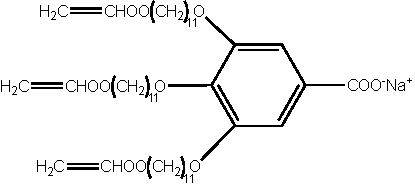
\includegraphics[width=\textwidth]{NaGA3C11.pdf}
  \caption{}\label{fig:monomer_structure}
  \end{subfigure}
  \begin{subfigure}{0.5\textwidth}
  \centering
  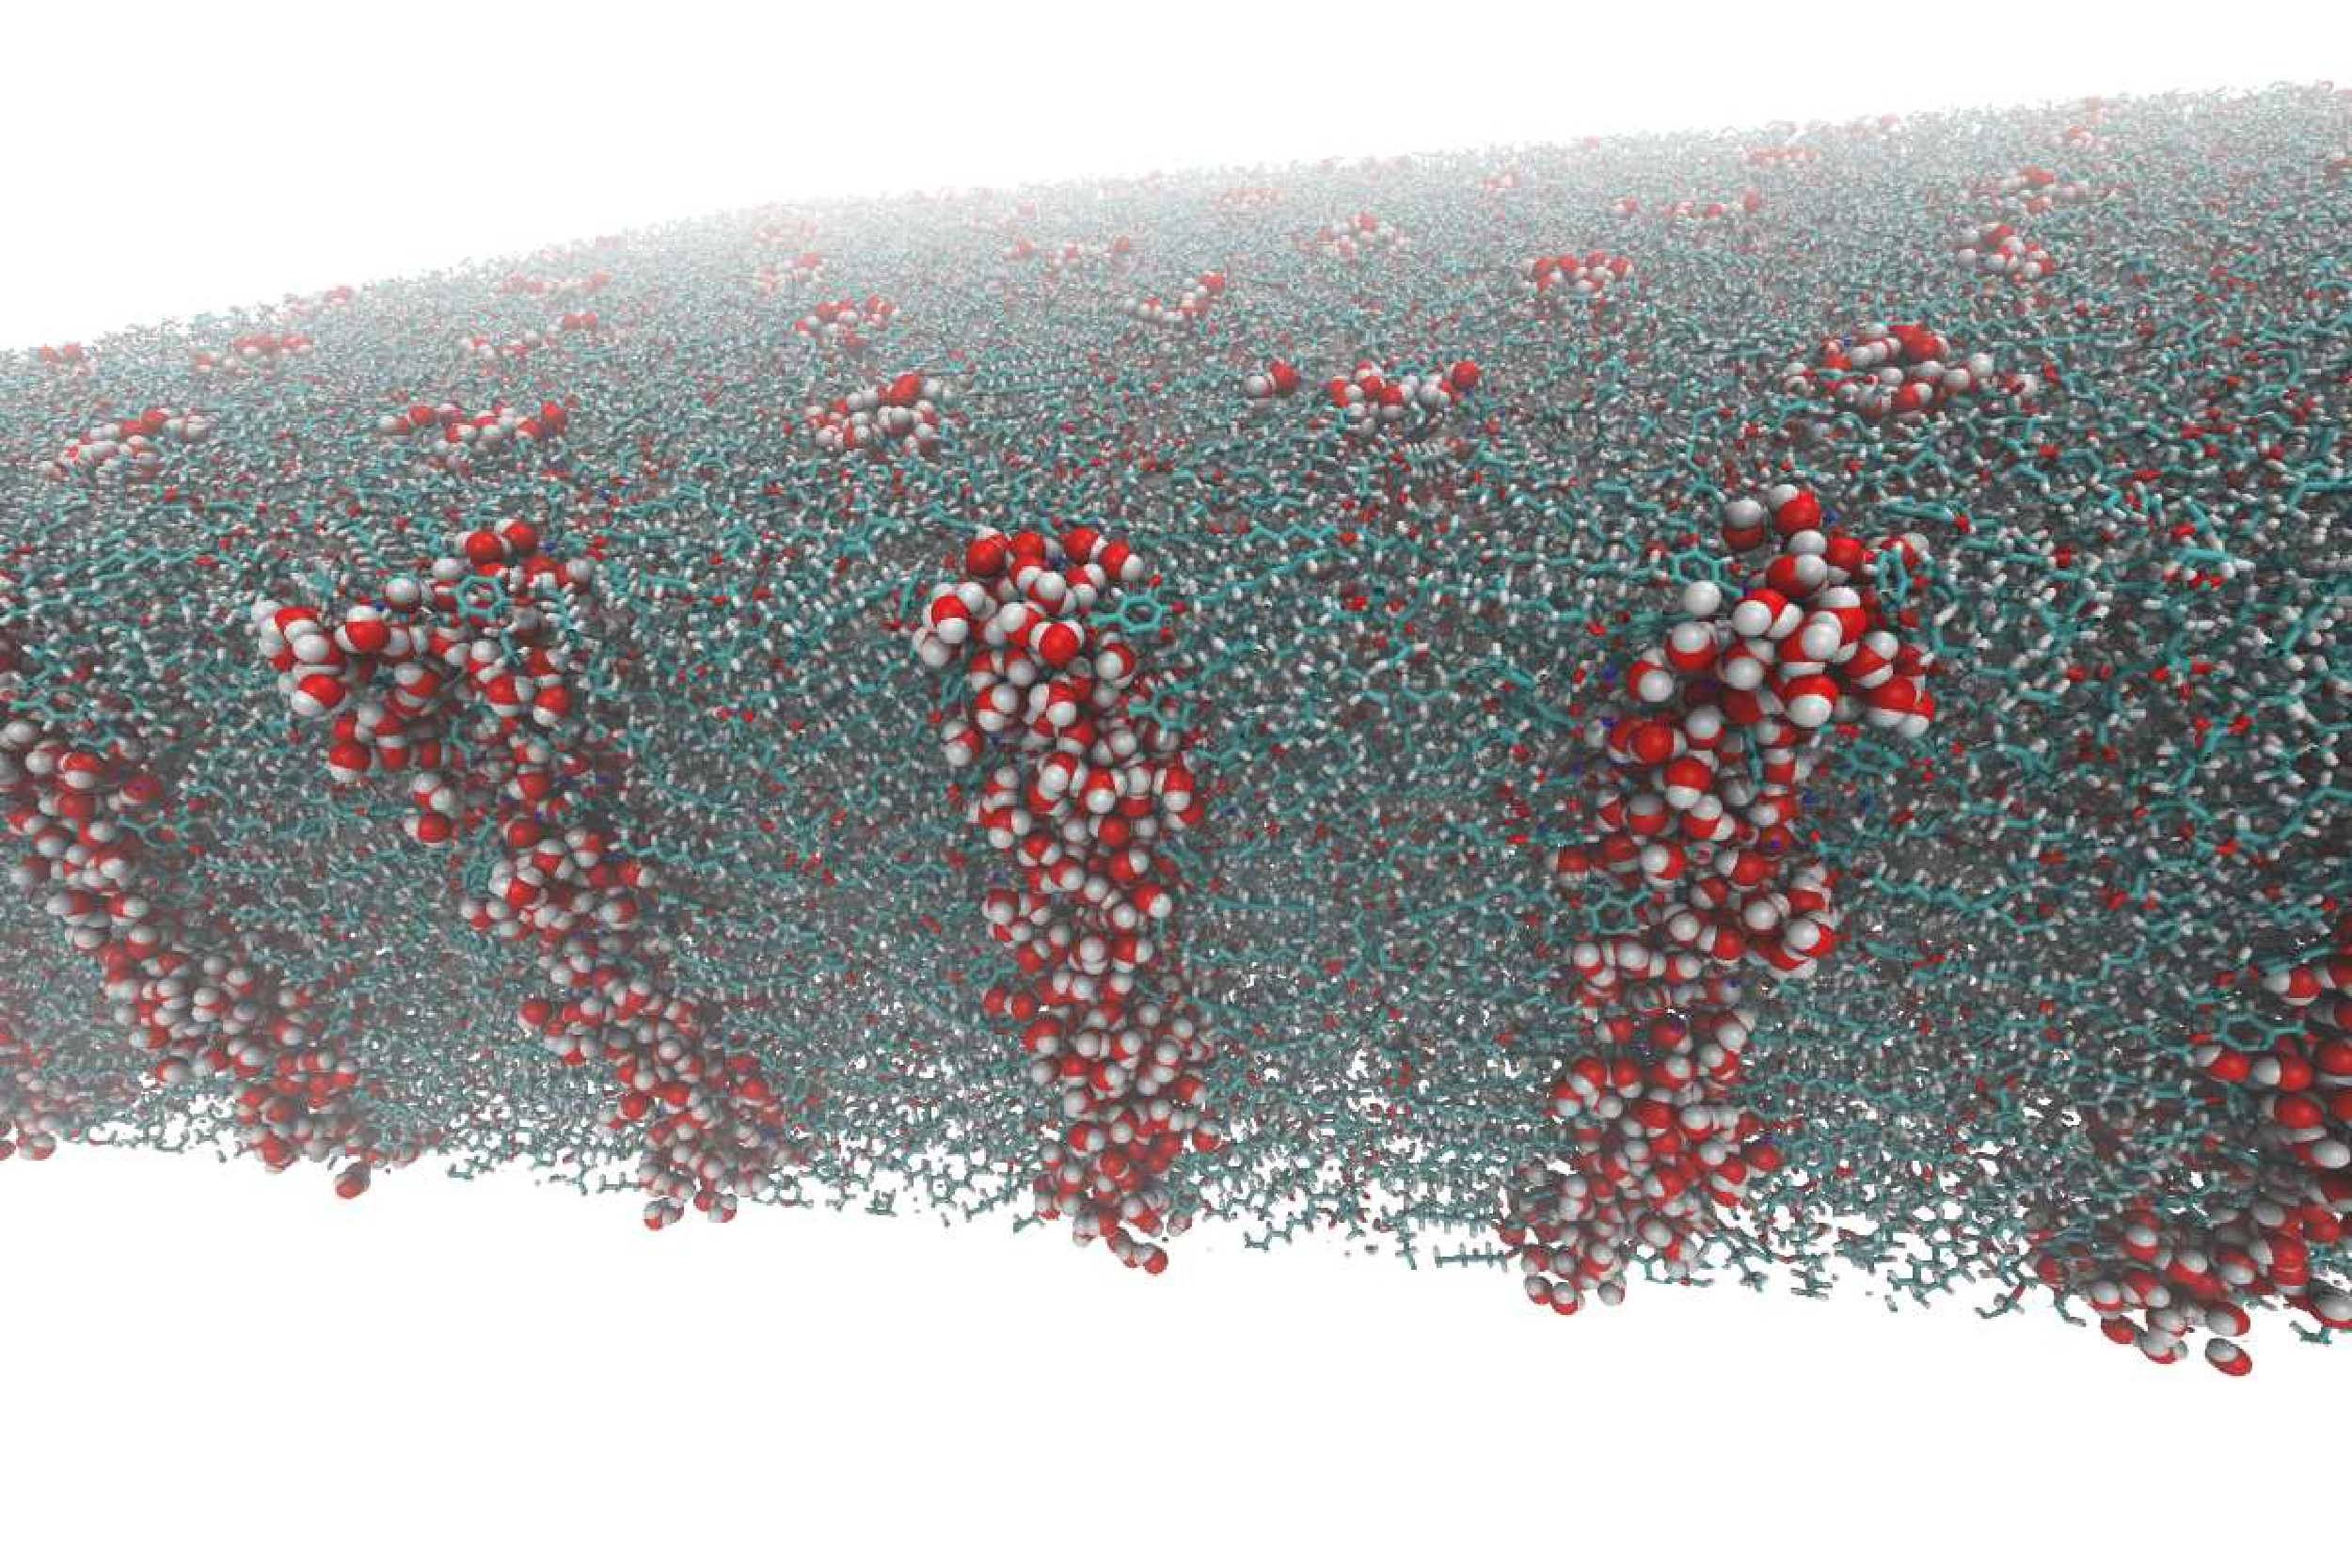
\includegraphics[width=\textwidth]{membrane_profile.pdf}
  \caption{}\label{fig:membrane_profile}
  \end{subfigure}
  \caption{(a) The wedge-shaped liquid crystal monomer Na-GA3C11 will form the inverted
  hexagonal phase in the presence of water where the carboxylate head groups occupy the
  pore centers. (b) A cross-section of a periodically replicated atomistic unit cell 
  used for simulations in this study reveals the membrane's aqueous, hexagonally packed,
  straight and uniform sized pores. Water present in the 
  %MRS6: isn't distal tail redundant? 
  distal tail region is omitted 
  for clarity.}\label{fig:membrane_structure}
  \end{figure}
  
  We chose to study a subset of the 4 fastest moving solutes from our previous
  work: methanol, acetic acid, urea and ethylene glycol. For each solute we 
  created a separate system and to each system we added 6 solutes per pore 
  for a total of 24 solutes. This number of solutes per pore provides a balance
  of a low degree of interaction between solutes, since we are primarily interested 
  in solute-membrane interactions at present, as well as a sufficient amount of 
  data from which to generate statistics on the time scales which we simulate.
  Further details on the setup and equilibration of these systems are described in
  our previous work.\cite{coscia_chemically_2019}
  
  We extended the 1 $\mu$s simulations of our previous work to 5 $\mu$s in order
  to collect ample data. We simulated the system with a time step of 2 fs at a pressure
  of 1 bar and 300 K controlled by the Parrinello-Rahman barostat and the v-rescale 
  thermostat respectively. We recorded frames every 0.5 ns.
  
  We considered each system to be equilibrated when the solute partitioning between the 
  pore and tail region reached apparent equilibrium and use only data after that point
  in our analysis of solute kinetics. We plot the solute partition versus time in
  Figure~\ref{S-fig:equilibration} of the Supporting Information in order to justify 
  our choice of equilibration times for each solute.

  \subsection{The Anomalous Diffusion Model}\label{method:model_sFBM}

  Solutes in this system 
  %MRS6: added
  very clearly 
  exhibit 
  subdiffusive behavior, a type of anomalous diffusion.
  During an anomalous diffusion process, the mean squared displacement (MSD)
  does not grow linearly with time, but instead it follows a power law of the form:
  %MRS6: do you need the subscript for $\alpha$? makes it harder to read. 
  \begin{equation} 
  \langle z^2(t) \rangle = K_{\alpha_d}t^{\alpha_d}
  \label{eqn:msd_form}
  \end{equation} 
  where $\alpha_d$ is the anomalous exponent and $K_{\alpha_d}$ is the generalized 
  diffusion coefficient. We only calculate MSD with respect to the solutes' center of
  mass $z$-coordinate, which is oriented along the pore axis. A value of $\alpha_d < 1$
  indicates a subdiffusive process, while values of $\alpha_d = 1$ and $\alpha_d > 1$ 
  are characteristic of Brownian and superdiffusive motion respectively.
  
  %MRS6: next paragraph could be clearer.  Maybe motivate at the beginning why the importance of time. vs. ensemble averated. It's sprung a sort of a surprise there's a difference 
  We analyzed the time-averaged MSD of the simulated trajectories by measuring
  all possible displacements over time lag $\tau$:
  \begin{equation}
  \overline{z^2(\tau)} = \dfrac{1}{T - \tau}\int_{0}^{T - \tau} (z(t + \tau) - z(t))^2 dt
  \end{equation}
  where T is the length of the trajectory. Note that only the \textit{ensemble} MSD
  will reproduce the form of Equation~\ref{eqn:msd_form} in all cases. The ensemble
  MSD is given by:
  \begin{equation}
  \langle z^2(t) \rangle = \langle z(t) - z(0) \rangle^2
  \label{eqn:ensemble_msd}
  \end{equation} 
  In a pure CTRW, for example, the power law distribution of trapping times leads to
  weak ergodicity breaking. In this case, the time-averaged MSD is linear while the ensemble averaged
  MSD has the form of Equation~\ref{eqn:msd_form}.~\cite{meroz_toolbox_2015} With power
  law trapping behavior, the time between hops diverges so there is no characteristic
  measurement time scale of solute motion. In fact, as measurement time increases, the 
  average MSD of a CTRW tends to decrease, a phenomenon called aging, because trajectories 
  with trapping times on the order of the measurement time get incorporated into the 
  calculation.~\cite{bel_weak_2005} We chose to analyze just the time-averaged MSD 
  because, compared to the ensemble average, it is a more statistically robust measure
  of the average distance a solute travels over time. 
  %MRS6: does it correspond properly to the physical situation of entry into the pore of new particles at each unit time?
  Although theoretically possible, we do
  not use the MSD to calculate $\alpha_d$ because we can extract the same parameter 
  with higher precision using the dwell time distributions as described below.
  
%  of the process is exhibits weak ergodicity breaking due to 
%  If the underlying subdiffusive process is not ergodic, like a pure CTRW, the time
%  averaged MSD becomes linear.
  
  \subsubsection{Subordinated Fractional Brownian Motion}\label{method:sfbm}

%  BJC4: I say something to the following effect in the intro
%  The solute motion in the system studied here may be consistent with 
%  subordinated fractional Brownian motion (sFBM) where the parent process is FBM and 
%  the leading process is a CTRW. We observe hopping and trapping which is consistent
%  with a CTRW, along with negatively correlated hops which is consistent with FBM.  

%  We modeled solute motion as a continuous time random walk (CTRW) subordinate to 
%  fractional Brownian motion, also called subordinated fractional Brownian motion (sFBM).
%  We modeled solute motion as a CTRW subordinate to FBM, also called sFBM. 
  
  One can characterize the CTRW component of an sFBM process by the parameters which describe
  its dwell time and hop length distributions. We used the \texttt{ruptures} Python
  package in order to automatically identify mean shifts in solute trajectories, 
  indicating hops.\cite{truong_ruptures:_2018} We used the corresponding hop lengths
  and dwell times between hops to construct empirical distributions.
  
  \textit{Dwell time distributions:} For subdiffusive transport, the distribution 
  of dwell times is expected to fit a power law distribution 
  proportional to $t^{-1-\alpha_d}$.~\cite{meroz_toolbox_2015}
  Because we are limited to taking measurements at discrete intervals dictated by the output 
  frequency of our simulation trajectories, we fit the empirical dwell times
  to a discrete power law distribution whose maximum likelihood $\alpha_d$ 
  parameter we calculated by maximizing the likelihood function: 
  \begin{equation}
	\mathcal{L}(\beta) = -n\ln \zeta(\beta, t_{min}) -
	\beta\sum_{i=1}^{n} \ln t_i 
  \label{eqn:powerlaw_likelihood}
  \end{equation}
  where $\beta = 1 + \alpha_d$, $t_i$ are collected dwell time data points,
  $n$ the total number of data points, and $\zeta$ is the Hurwitz zeta function
  where $t_{min}$ is the smallest measured value of	$t$.~\cite{clauset_power-law_2009}
  
  In practical applications, the heavy tail of power law distributions can result in 
  arbitrarily long dwell times that are never observed in MD simulations. We cannot
  observe dwell times longer than the length of a single trajectory. 
  In order to directly compare our anomalous diffusion model to finite-length MD 
  trajectories we need to bound the dwell time distribution. We do this by adding 
  an exponential cut-off to the power law so the dwell time distribution is 
  now proportional to $t^{-1 - \alpha_d}e^{-\lambda t}$.
  %MRS6: are there papers to cite that this is a standard way to cut them off (i.e. rather than truncate, etc).
  % of the form:
%  \begin{equation}  %BJC3: maybe make this equation in line? Else move regular power law to its own equation
%    p(t) \propto t^{-1 - \alpha}e^{-\lambda t}
%  \label{eqn:powerlaw_cutoff}
%  \end{equation}
  We determine MLEs of $\alpha_d$ and $\lambda$ by maximizing the likelihood function:~\cite{clauset_power-law_2009}
  \begin{equation}
    \mathcal{L}(\alpha_d, \lambda) = n(1 - \alpha_d)\ln\lambda - n\ln\Gamma(1 - \alpha_d, t_{min}\lambda) - \alpha_d\sum_{i=1}^{n}\ln t_i - \lambda\sum_{i=1}^n t_i
  \label{eqn:powerlaw_cutoff_likelihood}
  \end{equation}
  
  \textit{Correlated hop length distributions:} The marginal distribution of hops by solutes 
  undergoing an sFBM process is Gaussian, therefore we parameterize it by its standard deviation, 
  $\sigma$.~\cite{metzler_random_2000, metzler_anomalous_2014,neusius_subdiffusion_2009}
  The measured mean is always very close to zero so we assume that it is exactly zero
  in our time series simulations since we have no reason to expect drift in either direction
  based on pore symmetry.

  % BJC3: Making a logical argument regarding how we estimate H here is important
  % because I haven't seen anyone do it this way.
  sFBM implies that hops are correlated which we describe using the Hurst parameter, $H$. 
  The autocovariance function of hop lengths has the analytical form:~\cite{mandelbrot_fractional_1968}
  \begin{equation}
    \gamma(k) = \dfrac{\sigma^2}{2}\bigg[|k-1|^{2H} - 2|k|^{2H} + |k+1|^{2H}\bigg]
  \label{eqn:fbm_autocorrelation}
  \end{equation}
  where $\sigma^2$ is the variance of the underlying Gaussian distribution from which hops are
  drawn and $k$ is the time lag, or number of increments between hops. The hop autocorrelation
  function is simply Equation~\ref{eqn:fbm_autocorrelation} normalized by the variance. 
  When $H < 0.5$, hops are negatively correlated, when $H = 0.5$ we recover Brownian motion
  and when $H > 0.5$, one observes positive correlation between hops. There are many methods
  for estimating the Hurst parameter for a time series.~\cite{clegg_practical_2006} It can
  be a difficult task because Equation~\ref{eqn:fbm_autocorrelation} decays slowly to zero, 
  especially when $H > 0.5$, meaning one needs to study large time lags with high frequency.
  Fortunately (from a mathematical perspective), all of our solutes show anti-correlated motion, so most of the information in
  Equation~\ref{eqn:fbm_autocorrelation} is contained within the first few time lags (see 
  Figure~\ref{S-fig:hurst_autocorrelation} of the Supporting Information). Any hope of
  fitting longer time lags to our data is lost in the noise since the analytical values
  are so close to zero. Therefore, we obtained H by performing a least squares fit of 
  Equation~\ref{eqn:fbm_autocorrelation} to the first 
  ten  
  0.5 ns time lags of the 
  empirically measured autocorrelation function.

  \subsubsection{Subordinated Fractional L\'evy Motion}\label{method:sflm}
  %MRS6: maybe make it clearer that this is something you will be doing in the paper 
  Since we also want to account for the possibility that
  %If the 
  distribution of hops is not Gaussian, we can model them with the
  more general class of L\'evy stable distributions. For independent and identically
  distributed random variables, the generalized central limit theorem assures 
  convergence of the associated probability distribution function (PDF) to a 
  L\'evy stable PDF. \cite{klages_anomalous_2008} The characteristic equation which 
  describes the Fourier transform of a L\'evy stable PDF is:
  %MRS6: maybe use just $\alpha$ for the general subdiffusive case, and alpha_h here.   
  \begin{equation}
    p_{\alpha_h, \beta}(k;\mu,\sigma) =\exp\left[i\mu k - \sigma^{\alpha_h}|k|^{\alpha_h}\left(1 - i\beta\frac{k}{|k|}\omega(k, \alpha_h)\right)\right]
  \end{equation}
  where \\
  \[\omega(k, \alpha_h) = \begin{cases}
  	\tan{\frac{\pi \alpha_h}{2}} & \text{if}~\alpha_h \neq 1, 0 < \alpha_h < 2, \\
  	-\frac{2}{\pi}\ln |k| & \text{if}~\alpha_h = 1
  	 \end{cases}
  \]
  $\alpha_h$ is the index of stability or L\'evy index, $\beta$ is the skewness 
  parameter, $\mu$ is the shift parameter and $\sigma$ is a scale parameter. The most
  familiar case, and one of three that can be expressed in terms of elementary functions,
  is the Gaussian PDF ($\alpha_h$ = 2, $\beta$ = 0). We assume symmetric distributions
  centered about 0 implying that $\beta$ and $\mu$ are both 0.
  
  Assuming hops are correlated, solute behavior may be described by subordinated 
  fractional L\'evy motion (sFLM). The Hurst parameter can again be used to describe
  hop correlations because they share the same autocorrelation structure.~\cite{tikanmaki_fractional_2010}
  The autocovariance function for FLM is:
  \begin{equation}
    \gamma(k) = \dfrac{C}{2}\bigg[|k-1|^{2H} - 2|k|^{2H} + |k+1|^{2H}\bigg],
    ~C = \frac{E\big[L(1)^2\big]}{\Gamma(2H + 1)\sin(\pi H)}
    \label{eqn:flm_autocovariance}
  \end{equation}
  where $E\big[L(1)^2\big]$ is the expected value of squared draws from the 
  underlying L\'evy distribution, effectively the distribution's 
  variance.~\cite{bishwal_maximum_2011} In general, most L\'evy stable distributions
  have an undefined variance due to their heavy tails. However, normalizing
  Equation~\ref{eqn:flm_autocovariance} by the variance of a finite number of draws
  from a L\'evy stable distribution results in the same autocorrelation structure as FBM.
  See Section~\ref{S-section:H_estimate} of the Supporting Information for numerical
  simulations illustrating this point.  % BJC3: could use another reference proving mathematically what I show numerically
  
  Analogous to power law dwell times, the heavy tails of L\'evy stable 
  hop length distributions result in rare but arbitrarily long hops. These long
  and unrealistic hops result in over-estimated simulated MSDs. We observe that
  the distribution of hops observed in our MD simulations are well approximated 
  by L\'evy stable distributions close to the mean, but they significantly under-sample
  the tails. We chose to truncate the L\'evy stable distributions based
  on where the theoretical probability distribution function (PDF) starts to 
  deviate from the empirically measured PDF (see Section~\ref{S-section:truncation}
  of the Supporting Information).~\cite{mantegna_stochastic_1994}

  \subsubsection*{Multiple Anomalous Diffusion Regimes}
  
  We observe different dynamical behavior when solutes move while inside 
  the pore versus while in the tail region. This suggest two anomalous diffusion 
  models of varying complexity. We created a simple, single mode model with a single 
  set of parameters fit to solute trajectories.
%  $\alpha$, $\sigma$, $H$ and, when the truncated power law is used, $\lambda$ parameters
%  fit to solute trajectories.
  Our second, two mode model assigns a set of parameters to each of 2 modes based
  on the solute's radial location. Solutes in mode 1 are in the pore region, defined
  %MRS4: some justification on why 0.75 vs. any other cutoff.
  %BJC4: I justified sentence after next. 
  as less than 0.75 nm from any pore center. All else are in mode 2, the tail region. 
  We determined this cut-off by maximizing the difference in dynamical behavior as 
  described in our previous work.~\cite{coscia_chemically_2019} Unfortunately, 
  there were not enough sufficiently long sequences of hops in each mode to reliably
  calculate a Hurst parameter for each mode so we used the Hurst parameter from the 
  single mode model for both modes of the two mode model.
  
  % BJC3: A small figure describing above might be useful, or maybe point to a figure in supporting info
 
  For the two mode model, we defined a transition matrix describing the rate at
  which solutes moved between the tail and pore region. We assumed Markovian transitions
  between modes, meaning each transition had no memory of previously visited modes. 
  We populated a 2$\times$2 count matrix by incrementing the appropriate entry by 1 each time step. 
  For example, if we observed the solute in the tails followed by a transition to 
  the pores, we incremented the $(2, 1)$ entry of the count matrix by 1. We generated
  the transition probability matrix from the count matrix by normalizing the 
  entries in each row so that they summed to unity.
 
  %MRS4: Do you assume Markovian behavior in transitions between the states?  Be explicit.
  %BJC4: Yes, added sentence directly after thesis above
  
  \subsubsection*{Simulating Anomalous Diffusion}

  We simulated models with all combinations of the types of dwell and hop length
  distributions described above, which are summarized in Table~\ref{table:anomalous_models}.
  All models include correlation between hops.

  \begin{table}[!htb]
	  \centering
	  \begin{tabular}{|c|c|c|}
	  \hline
	  Dwell Distribution                & Hop Length Distribution & Abbreviation \\
	  \hline
      Power Law                         & Gaussian                & sFBM         \\
      Power Law w/ Exponential Cut-off  & Gaussian                & sFBMcut      \\
      Power Law                         & L\'evy Stable           & sFLM         \\
      Power Law w/ Exponential Cut-off  & L\'evy Stable           & sFLMcut      \\
	  \hline
	  \end{tabular}
	  \caption{We tested models with various modifications to the dwell and hop
	  length distributions. We incorporate correlation structure into all models.}\label{table:anomalous_models}
 \end{table}

  % BJC3: will need to modify this text to reflect different lengths of simulations
  For each solute, we simulated 1,000 anomalous diffusion trajectories of length
  $T_{sim}$ in order to directly compare our model's predictions to MD simulations.
  $T_{sim}$ varied 
  %MRS6:
  between solutes
  due to differing solute equilibration times. We constructed 
  trajectories by simulating sequences of dwell times and correlated hop lengths
  generated based on parameters randomly chosen from our bootstrapped parameter 
  distributions. We propagated each trajectory until the total time equaled or 
  exceeded $T_{sim}~ \mu$s, then truncated the last data point so that the total 
  time exactly equaled $T_{sim}~ \mu$s since valid comparisons are only possible 
  between fixed length sFBM simulations. 
  % BJC4: removed following sentence because I talk about aging above
  %The power law dwell time behavior gives rise to the aging phenomenon, embodied by a 
  %decrease in MSD with measurement time.~\cite{neusius_subdiffusion_2008,metzler_anomalous_2014}
  We reported the time-averaged MSD up to a 1000 ns time lag corresponding 95\% confidence
  intervals. 
  
  When simulating 2 mode models, we determined the state sequence based on random 
  draws weighted by the appropriate row of the probability transition matrix. We then
  drew hops and dwells based on the current state of the system. Since we calculated
  the transition probabilities from a finite data set, they have an associated 
  uncertainty which we 
  %MRS4: not quite sure what you mean by incorporating uncertainty. 
  %BJC4: Added comment about having a finite amount of data with which to create transition matrix. Therefore it is uncertain
  incorporated by re-sampling each row from a two dimensional Dirichlet distribution
  %MRS6:
  %(also called a 
  (which is also a 
  beta distribution for the 2D case) with concentration parameters 
  defined by the count matrix.~\cite{bacallado_bayesian_2009}

  %BJC4: already said this earlier
%  We used a single Hurst parameter to describe
%  correlation between hops, independent of the solute's mode. Ideally, each mode
%  would have its own Hurst parameter, but we did not observe enough long sequences
%  of uninterrupted time spent in each mode with which to generate robust
%  autocorrelation functions. 
  
  %BJC3: not sure how to cite fbm
  We used the Python package \texttt{fbm} to generate exact simulations of FBM and our
  own Python implementation of the algorithm by Stoev and Taqqu to simulate FLM.
  \cite{stoev_simulation_2004} Note that, to our knowledge, there are no known exact
  simulation algorithms for generating FLM trajectories. 
  %MRS6: broke sentence
  However, the algorithm
  we used sufficiently approximates draws from the marginal distribution and 
  reasonably approximates the correlation structure on MD simulation timescales. We
  added an empirical correction to enhance the accuracy of the correlation structure
  (see Section~\ref{S-section:flm_correlation} of the Supporting Information for 
  validation of the approach).
  %MRS6: suggest in the supporting information describe what measure was used to determine that the algorithm sufficiently and reasonably approxmiates.
%  When simulating 5 $\mu s$ FLM trajectories, we limited the maximum hop length to
%  be no larger than the largest hop observed in our MD simulations. L\'evy stable 
%  distributions often have heavy tails and an undefined variance which can give 
%  rise to arbitrarily long particle displacements. We do not observe hops longer 
%  than x nm in our simulations which emphasizes that these distributions are only 
%  an approximation. We avoid enormous and unrealistic hops problem by truncating 
%  the tails of the distribution.

%  An important feature 
%  of L\'evy distributions is their heavy tails. Generally, a lower L\'evy index is 
%  characteristic of heavier tails, meaning higher probabilities of extremely large jumps.
%  In practical applications these extremely large hop lengths are unrealistic, especially
%  when comparing to MD.

%  BJC4: I already said this above
%  When simulating MD-length FLM trajectories, we limited the maximum hop length based on where
%  the empirical hop distribution began to significantly under-sample the theoretical
%  maximum likelihood estimate (MLE) L\'evy stable distribution (see 
%  Section~\ref{S-section:truncation} of the Supporting Information).

%  For our 1 second simulations, we limited the maximum hop length to that seen by
%  the same solute undergoing Brownian motion in an unconfined aqueous environment. 
%  We have no reason to believe there is any kind of facilitated diffusion, so 
%  excursions characteristic of Brownian motion represent a reasonable upper limit
%  on hop lengths. To determine these limits we placed 24 solutes in a cubic box of 
%  water, 4 nm on each side. We allowed the solutes to diffuse for 100 ns, more than
%  ensuring the mean squared displacement entered a linear regime. We recorded the largest
%  observed hop length over a 0.5 ns time lag. 

  \subsection{The Markov State-Dependent Dynamical Model}\label{method:MSMs}  

  A Markov state model (MSM) decomposes a time series into a set of discrete states
  with transitions between states defined by a transition probability matrix, $T$,
  which describes the conditional probability of jumping to a specific state given
  the previously observed state.~\cite{pande_everything_2010,wehmeyer_introduction_2018}
  %MRS6: maybe skip this next sentence since you don't actually use them?
  Software packages such as MSMbuilder~\cite{beauchamp_msmbuilder2:_2011} and 
  pyEMMA~\cite{scherer_pyemma_2015} provide work flows capable of featurization and
  dimensional reduction which are often necessary to identify representative states.

  In this work, we define a total of 8 discrete states based on the 3 trapping
  mechanisms observed in our previous work. Therefore, there is no need to 
  apply any algorithmic approaches to identify and decompose our system into 
  discrete states. The states we have chosen include all combinations of trapping
  mechanisms in the pore and out of the pore (see Table~\ref{table:states}). They
  assume that there are no significant kinetic effects resulting from solute 
  conformational changes or pore size fluctuations. 
  %MRS6:
  %Eh, Don't need to talk about future work. 
  %an assumption that may be relaxed in future work. 

  

  We use the same radial cut-off (0.75 nm) as in the 
  anomalous diffusion model to differentiate the pore and tail region.  We define 
  a hydrogen bond to exist if the distance between donor, D, and acceptor, A, 
  atoms is less than 3.5 \AA~and the angle formed by $D-H \cdots A$ is less than
  30$\degree$. We define a sodium ion to be associated with an atom if they are 
  within 2.5 \AA~of each other, 
  %MRS6:
  as determined in our previous work~\cite{coscia_chemically_2019}
  
  \begin{table}[!htb]
	  \centering
	  \begin{tabular}{|l|l|}
	  \hline
	  1. In tails, not trapped                     & 5. In pores, not trapped                     \\
	  2. In tails and hydrogen bonding             & 6. In pores and hydrogen bonding             \\
	  3. In tails and associated with sodium       & 7. In pores and associated with sodium       \\
	  4. In tails, hydrogen bonding and associated & 8. In pores, hydrogen bonding and associated \\
	  \hline
	  \end{tabular}
	  \caption{We defined 8 discrete states based on all combinations of previously observed solute
	  trapping mechanisms.}\label{table:states}  
	  %BJC3: the caption will depend on the journal. I don't
	  % like that J Phys Chem B forces the captions as titles, but if we choose them I think it would
	  % be cleaner to make the caption more title-like.
  \end{table}
  
  We constructed the state transition probability matrix, $T$, based on observed solute trajectories.
  Using methods described in our previous work, we determined each solute's radial location 
  and which, if any, trapping mechanisms affected it at each time step, then assigned the 
  observation to a specific state according to the definitions in Table~\ref{table:states}.~\cite{coscia_chemically_2019}
  Analogous to the mode transition matrix in Section~\ref{method:model_sFBM}, and based on
  the current and previous state observation, we incremented the appropriate entry of an
  $n~\times~n$ count matrix by 1, where $n$ is the number of states.
  
  %MRS4: here, be more explicit you are testing the validity of the Markovian approximation on the molecular data.
  %BJC4: Tried to clarify in thesis statement. Let me know if you think it needs more
  We verified the Markovianity of state transitions by solutes in our MD simulations 
  by analyzing the empirically measured transition matrix. An important condition
  of a Markov process is the satisfaction of detailed balance:
  \begin{equation}
  T_{i,j}P_i(t=\infty) = T_{j,i}P_j(t=\infty)
  \end{equation}
  where $P$ is the equilibrium distribution of states. In other words, the number of
  transitions from state $i$ to $j$ and from state $j$ to $i$ should be equal. A second
  test is to verify that $T$ holds up to coarser time scale partitioning. As long as solutes
  sufficiently sample the states in Table~\ref{table:states}, $T$ should be invariant
  with time.~\cite{swope_describing_2004} We verified these properties 
  in Section~\ref{S-section:markov_validation} of the Supporting Information.
  
  Adding to the standard MSM framework, we incorporated the dynamics of the solutes
  within each state as well as the dynamics of state transitions, which includes the
  overall configurational state of the solute and it's environments. 
  While MSMs are often used to estimate equilibrium populations of various states, adding 
  state-dependent dynamics allows us to simulate solute trajectories.
  %BJC5: I said below already, but I still think it belongs
  Hence why we refer to them as Markov State-Dependent Dynamical Models (MSDDMs). 
  
  We recorded the $z$-direction displacement at each time step in order to construct 
  individual emission distributions for each state and transition between states. 
  This results in 64 distinct emission distributions with some far more populated than
  others. We modeled all of the emission distributions as symmetric L\'evy stable 
  distributions in order to maintain flexibility in parameterizing the distributions.
  
  We use the Hurst parameter to describe this negative time series correlation.
  However, there is not sufficient data to accurately measure a Hurst parameter for 
  each type of transition. We avoided this problem by combining all distributions 
  associated with state transitions and treating all transitions as correlated
  emissions from a single L\'evy stable distribution. This reduces the number of emission
  distributions from 64 to 9 (1 for each of the 8 states and 1 for transitions between states).  
  
%  We observed negatively correlated hops within each state and among transitions between
%  states. We can use the Hurst parameter to describe this negative time series correlation
%  however, there is not sufficient data to accurately measure a Hurst parameter for 
%  each type of transition. We avoided this problem by treating transitions as correlated
%  emissions from a single L\'evy stable distribution. This reduces the number of emission
%  distributions from 64 to 9 (1 for each state and 1 for transitions between states).
  
  We simulated realizations of the MSDDM using the probability transition matrix and 
  emission distributions. For each trajectory simulated, we chose an initial state
  randomly from a uniform distribution. We generated a full state sequence by randomly
  drawing subsequent states weighted by the rows of the probability transition matrix
  corresponding to the particle's current state. Again, because we are working with a
  finite data set, we incorporated transition probability uncertainties into the rows
  of the transition matrix by resampling them from a Dirichlet distribution. For each 
  same-state subsequence of the full state sequence, we simulated an FLM process using
  the Hurst parameter of that state and the parameters of the corresponding emission
  distribution. Independently, we simulated the transition between each same-state 
  sequence with an FLM process based on the Hurst parameter of transition sequences 
  and the parameters of the single transition emission distribution. We used the same
  FLM simulation procedure described in Section~\ref{method:model_sFBM}.

%  corresponding emissions from the rows of the probability transition matrix and the 
%  appropriate emission distribution respectively. We added correlation between transitions
%  as well as to sequences of emissions while dwelling in specific states using the FLM
%  simulation procedure described in Section~\ref{method:model_sFBM}.

  %\subsection{Solute Flux}\label{method:mfpt}
  %MRS6: tweak to make more active
  \subsection{Estimating Solute Flux}\label{method:mfpt}
  
  We determined the rate at which solutes cross macroscopic-length pores based on the
  Hill relation:~\cite{hill_free_1989}
  \begin{equation}
  J = \frac{1}{MFPT}
  \label{eqn:hill_relation}
  \end{equation}
  where $J$ is the single particle solute flux and MFPT refers to the mean first passage
  time. To account for input concentration dependence of the flux, assuming that particles
  are uncorrelated, one can multiply Equation~\ref{eqn:hill_relation} by the total number
  of particles to get the total flux. In the context of our work, the MFPT describes the
  average length of time it takes a particle to move from the pore entrance to the pore exit. 
  
  We generated particle trajectories, parameterized with the above models, in order
  to construct a distribution of first passage times across a membrane pore of length $L$.
  For computational reasons dependent on the model used, we simulated 1,000-10,000 trajectory
  realizations, released at the pore entrance ($z=0$). In the case of 
  uncorrelated hops, one can continuously draw from the hop length distribution until 
  $z \geq L$ (or $-L$ for the sake of computational efficiency). The length of time 
  between the last time the particle crossed $z=0$ and the end of the trajectory gives a 
  single passage time. When particle hops are correlated, as they are in all cases of
  this work, we cannot continuously construct the particle trajectories. Rather, we must
  generate trajectories of length $n$ and measure the length of the sub-trajectory 
  which traverses from $0$ to $L$ without becoming negative.
  %BJC4: below is only necessary if you the mean of the distribution exists.
  %It is important to choose a value of $n$ sufficiently
  %large that all trajectories reach $L$, or else the mean first passage time will 
  %be underestimated. 
  
  We calculated the expected value of analytical fits to the passage time distributions
  in order to determine the MFPT for a given solute and pore length. One should not 
  use the mean of the empirical passage time distribution because it is highly likely
  that the true MFPT will be underestimated unless 100\% of a very large number of 
  trajectories reach $L$. If a trajectory does not reach $L$ within $n$ steps, it is
  possible that a very long passage time has been excluded from the distribution.
  
  %BJC4: can probably delete this paragraph
%  We are unaware of an analytical passage time distribution which describes our 
%  geometry. The setup of our system is consistent with a one dimensional interval 
%  with two absorbing boundaries. In the absence of an external force and with a constant
%  diffusion coefficient, $D$, the MFPT is simply:
%  \begin{equation}
%  T = \frac{z_0(L - z_0)}{2D}
%  \end{equation}
%  where $z_0$ is the initial position of particle trajectories.~\cite{gitterman_mean_2000}
%  Of course that implies a conventional MFPT of 0 since particles overwhelmingly exit the
%  pore at $z=0$. Therefore, we chose only to include trajectories in the MFPT calculation 
%  which cross the boundary at $L$. We are unaware of an analytical form of the MFPT or 
%  the distribution of passage times describing our system even in the simplest case of 
%  Brownian increments. %BJC4: still digging for an analytical solution. Rich said the 
%  %'marathon' runner problem might give a solution. It may be the same as the distribution
%  % of runners crossing the finish line
  
  To come up with an analytical equation describing the passage time distributions, 
  one can frame the 
  problem as a pulse of particles instantaneously released at the pore inlet ($z=0$)
  which moves at a constant velocity, $v$, and spreads out as it approaches $L$. 
  This spreading is parameterized by an effective diffusivity parameter, $D$. This 
  approach gives results equivalent to if we had released each particle individually
  and then analyzed the positions of the ensemble of trajectories as 
  a function of time. The analytical expression describing the distribution of 
  first passage times is:~\cite{cussler_diffusion:_2009}
  \begin{equation}
  P(t) = -\frac{1}{\sqrt{\pi}}e^{-(L - vt)^2 / (4Dt)}\bigg(-\frac{D(L - vt)}{4(Dt)^{3/2}} - \frac{v}{2\sqrt{Dt}}\bigg)
  \label{eqn:passage_times}
  \end{equation} 
  where the only free parameters for fitting are $v$ and $D$. A derivation
  of Equation~\ref{eqn:passage_times} is given in Section~\ref{S-section:fpt_derivation}
  of the Supporting Information. We calculated the expected value of 
  Equation~\ref{eqn:passage_times} in order to get the MFPT.
  
  %MRS5: I would put this next section up until just before Eq. 15 in the supporting information (keep any citations in the main text). 
  %BJC5: moved to supporting
%  To derive an analytical equation, first consider an initial pulse spreading out 
%  over time with a fixed mean. We can solve for the time-dependent probability density
%  of particle positions by solving the one dimensional diffusion equation:
%  \begin{equation}
%  \frac{\partial p}{\partial t} = D \frac{\partial^2 p}{\partial z^2}
%  \end{equation}
%  The appropriate initial and boundary conditions are:
%  $$BC1: t > 0, z = \infty, p = 0$$
%  $$BC2: t > 0, z = 0, \frac{\partial p}{\partial z} = 0$$
%  $$IC: t = 0, c = M\delta(z)$$
%  where $M$ is the total number of particles in the system. It has been shown 
%  elsewhere that the solution to this equation is:~\cite{cussler_diffusion:_2009}
%  \begin{equation}
%  p(z, t) = \frac{1}{\sqrt{4 \pi D t}}\exp\bigg(\frac{-z^2}{4Dt}\bigg)
%  \end{equation}
%  We can make the substitution $z = z - vt$, where $v$ represents a constant average
%  velocity, in order to linearly shift the mean as a function of time:
%  \begin{equation}
%  p(z, t) = \frac{1}{\sqrt{4 \pi D t}}\exp\bigg(\frac{-(z - vt)^2}{4Dt}\bigg)
%  \end{equation}
%  One can track the fraction of particles, $F$, that have crossed the pore 
%  boundary by integrating:
%  \begin{equation}
%  F(t) = \int_L^\infty p~dz = \mathrm{erfc}\bigg(\frac{L - vt}{2\sqrt{D t}}\bigg)
%  \end{equation}
%  where $L$ is the pore length. This represents the cumulative first passage 
%  time distribution so we take its derivative in order to arrive at the first
%  passage time distribution:

  We used the ratio of solute fluxes in order to determine membrane selectivity, $S_{ij}$,
  towards solutes. Selectivity of solute $i$ versus $j$ is defined in terms of the
  ratio of solute permeabilities, $P$:~\cite{guo_pervaporation_2004}
  \begin{equation}
  S_{ij} = \frac{P_i}{P_j}
  \end{equation}
  We can relate this to solute flux using Kedem and Katchalsky's equations for 
  solvent volumetric flux, $J_v$, and solute flux, $J_s$:~\cite{kedem_permeability_1963,al-zoubi_rejection_2007}
  %al-zoubi_rejection_2007 clarifies that these equations can be used for nanofiltration, ultrafiltration etc. by treating the membrane as a black box subject to irreversible thermodynamics.
  \begin{equation}
  J_v = L_p(\Delta P - \sigma\Delta \pi)
  \end{equation} 
  \begin{equation}
  J_s = P_s \Delta C + (1 - \sigma)CJ_v
  \label{eqn:solute_flux}
  \end{equation}
  where $L_p$ is the pure water permeability, $\Delta P$ and $\Delta \pi$ are the 
  trans-membrane hydraulic and osmotic pressure differences, $\sigma$ is the reflection
  coefficient, $P_s$ is the solute permeability, $\Delta C$ is the trans-membrane
  solute concentration difference and $C$ is the mean solute concentration. Since our
  simulations do not include convective solute flux, we eliminate the second term 
  of Equation~\ref{eqn:solute_flux} which allows us to derive a simple expression
  for selectivity in terms of solute flux:
  \begin{equation}
  S_{ij} = \frac{J_i / \Delta C_i}{J_j / \Delta C_j}
  \label{eqn:selectivity}
  \end{equation}
  
  
%    $$ A_i = \frac{J}{(\Delta P - \Delta \pi)} $$
%  $$ S = \frac{A_i}{A_j} for a given pore length, L$$
%  $$J = A(\Delta P - \Delta \pi)$$
%  $$A = \frac{P_i}{L} $$
%  $$P_i = \frac{flux}{drivingforce \cdot L} [=] \frac{particles}{s \cdot bar \cdot L}$$
  
  %BJC4: we have better ways of getting peaks now
%  In the absence of an analytical equation for the MFPT, we instead report the location of
%  the peak of the passage time distribution. This has the added advantage of treating
%  cases where the passage time distribution diverges and no mean exists. While we will
%  call the peak in the distribution the MFPT, it is important to recognize that this 
%  value is more representative of a typical passage time rather than a mean. 
  
  % BJC: concentration profile stuff
%  One would then segment the trajectory
%  each time it crosses $0$ and reflect all of the negative trajectories. The ensemble of
%  trajectories is consistent with the fraction of partic
  
%MRS6: maybe more subsections in results so people can get a sense of where the flow is going at a glance?
  \section{Results and Discussion}
  
  %BJC4: Not sure if I should start by commenting on the stationarity of the 
  %solute trajectories. I talk about it when I start validating with the train/test procedure.
  
%  \subsection{Stationarity of Solute Trajectories}\label{section:stationarity}
%  %BJC4: Maybe re-theme the section: applicability of model
%  
%  Before applying the model, it is important to analyze the MD trajectories
%  themselves in order to understand what conclusions one could reasonably to 
%  draw by applying these models. 
%  
%  %BJC4: this might belong with validation.
%  We observe that in many cases, the distribution of solutes within the membrane
%  evolves slowly with time. We defined the perceived equilibration time point 
%  for each solute based on the time at which the number of solutes inside the
%  pores and tails stabilized. Nonetheless, we observe evidence of non-stationary
%  solute behavior after equilibration on the $\mu$s timescale. In Table \_\_, we compare the MSD of the 
%  solutes calculated using trajectory data from the first and second halves of the
%  equilibrated simulation time. Ethylene glycol and methanol, show considerable
%  differences in their MSDs. Although the MSD calculated from both halves of the 
%  acetic acid trajectories are similar, their shapes are considerably different 
%  (see SI). Urea is the only solute in this study that demonstrates satisfactory
%  stationarity on the 5 $\mu$s timescale.
%  
%  The non-stationary behavior of each solute presents itself in different ways.
%  On average, methanol molecules in the tails appear to be drifting further 
%  away from the pore center with time. Ethylene glycol appears to experience an
%  increased incidence of long trapping times. The partition of acetic acid 
%  between the pores and tails oscillates slowly over time. These problems probably
%  cannot be addressed without more simulation time or additional solute trajectories. 
%  
%  In light of these observations, we chose to demonstrate the performance and insights
%  that could be gained from our models using all of solutes with complete data sets
%  collected after the perceived equilibration time. However, we only use urea to 
%  validate the model's predictive power and to estimate solute flux.
%    
%  There are a couple of ways to address this issue in the long term. The simplest
%  approach is to run the MD simulations longer. This option is likely not feasible
%  because the equilibration timescale in these systems is unknown for most of 
%  the solutes in the study, even after consider computational effort. A more 
%  sustainable approach, which would help screen any solute of interest, would 
%  require us to learn the equilibrium distribution of solutes in the membrane
  
  \subsection{Anomalous Diffusion Modeling}\label{section:sFBM}
  
  \subsubsection{Parameterizing Subordinated Fractional Brownian Motion}\label{section:AD_parameterization}

  The evidence suggests that solutes in this system can be well-modeled by subordinated
  fractional Brownian motion. In Figure~\ref{fig:anticorrelated_hops}, we use urea to
  support this claim. Analogous figures for all other solutes are presented in the Supporting
  Information, Figures~\ref{S-fig:GCL_anticorrelated_hops}--\ref{S-fig:MET_anticorrelated_hops}.
  The solutes clearly perform jumps after periods of relative
  immobility (see Figure~\ref{fig:solute_trajectories} for example). The near-Gaussian distribution
  of jump lengths and power law distribution of dwell times are both characteristic of 
  CTRWs (Figures~\ref{fig:hop_distribution_comparison} and~\ref{fig:powerlaw}). The apparent
  anti-correlation between hops suggests a fractional diffusion process is subordinate to the
  CTRW. We believe the subordinated process is FBM or FLM because their analytical correlation 
  structures are close to those observed in our simulations (Figure~\ref{fig:hop_acf}). Fractional
  motion is common in crowded viscoelastic environments where movement is highly influenced by
  the movement of surrounding components, such as monomer tails in our case.~\cite{ernst_fractional_2012}
  %The parameter estimates describing the 1 and 2 mode hop and dwell distributions are 
  %summarized in Figures~\ref{fig:1mode_parameters} and~\ref{fig:2mode_parameters}.
  
  \begin{figure}
  \centering
  %BJC3: included radial distance from pore center because I could. But does that make it look bad?
  % /figures/solute_trajectories.py
  \begin{subfigure}{0.45\textwidth}
  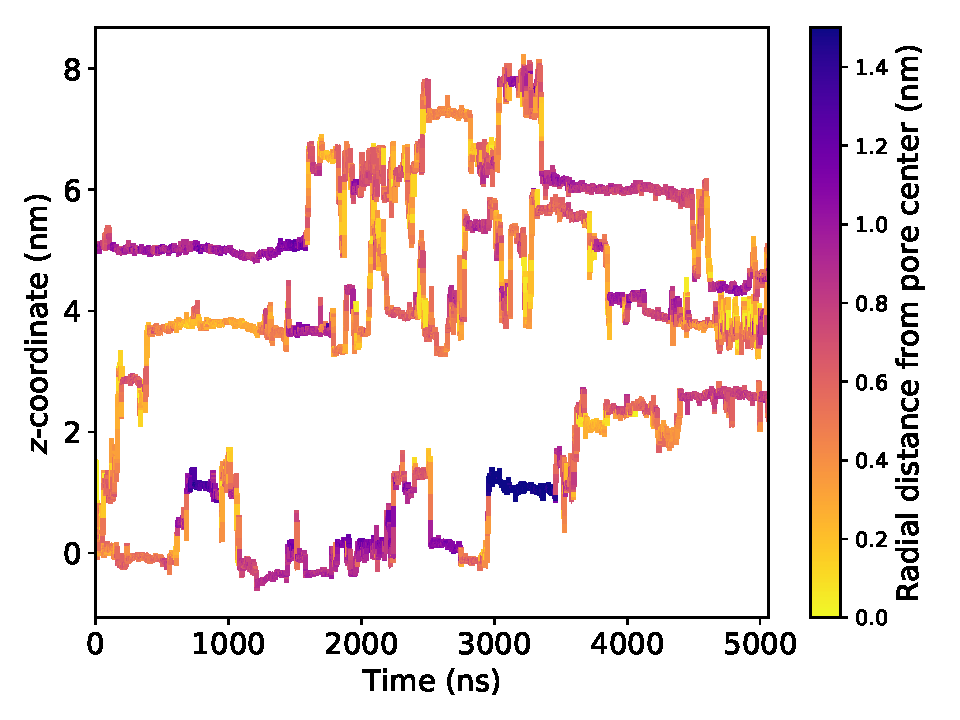
\includegraphics[width=\textwidth]{URE_trajectories.pdf}
  \caption{}\label{fig:solute_trajectories}
  \end{subfigure}
  % Next 3: /figures/sfbm_distributions
  \begin{subfigure}{0.45\textwidth}
  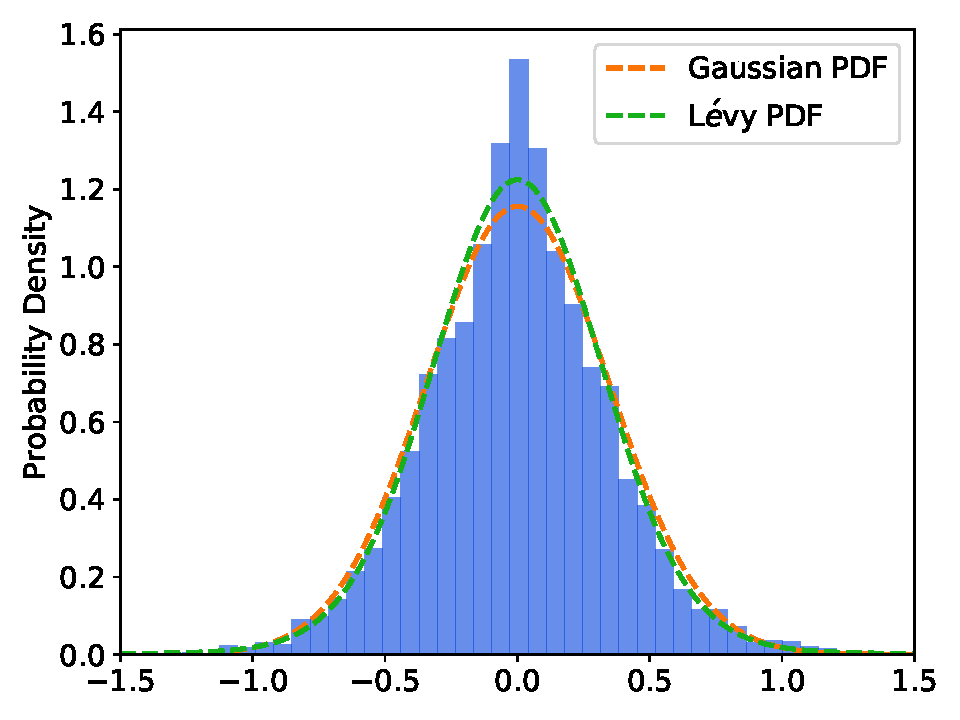
\includegraphics[width=\textwidth]{gaussian_levy_comparison_anomalous_GCL.pdf}
  \caption{}\label{fig:hop_distribution_comparison}
  \end{subfigure}
  \begin{subfigure}{0.45\textwidth}
  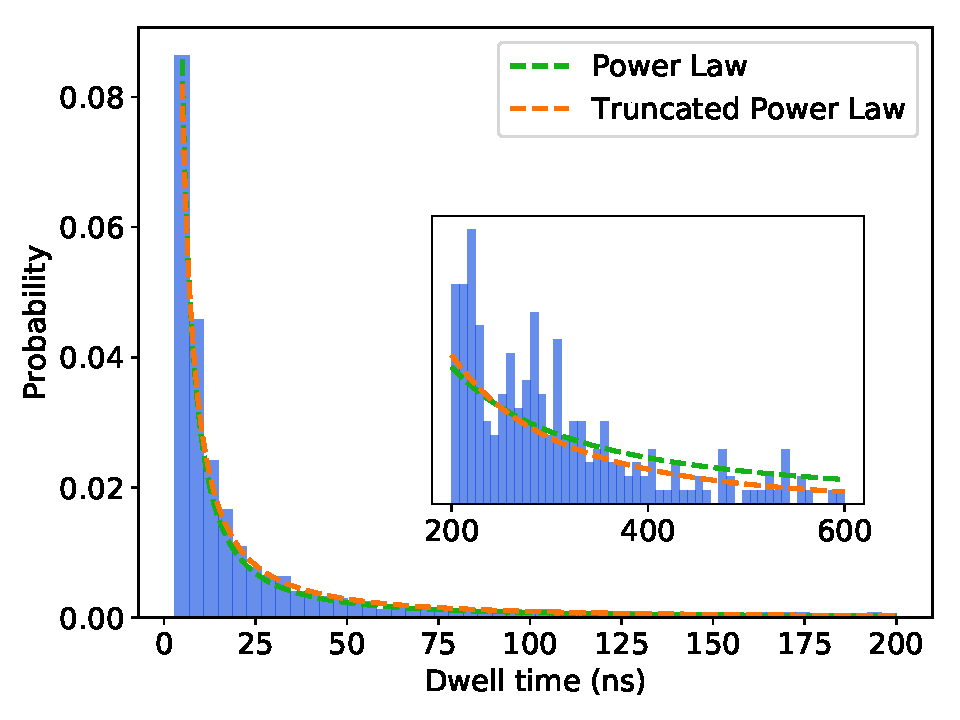
\includegraphics[width=\textwidth]{URE_powerlaw.pdf}
  \caption{}\label{fig:powerlaw}
  \end{subfigure}
  \begin{subfigure}{0.45\textwidth}
  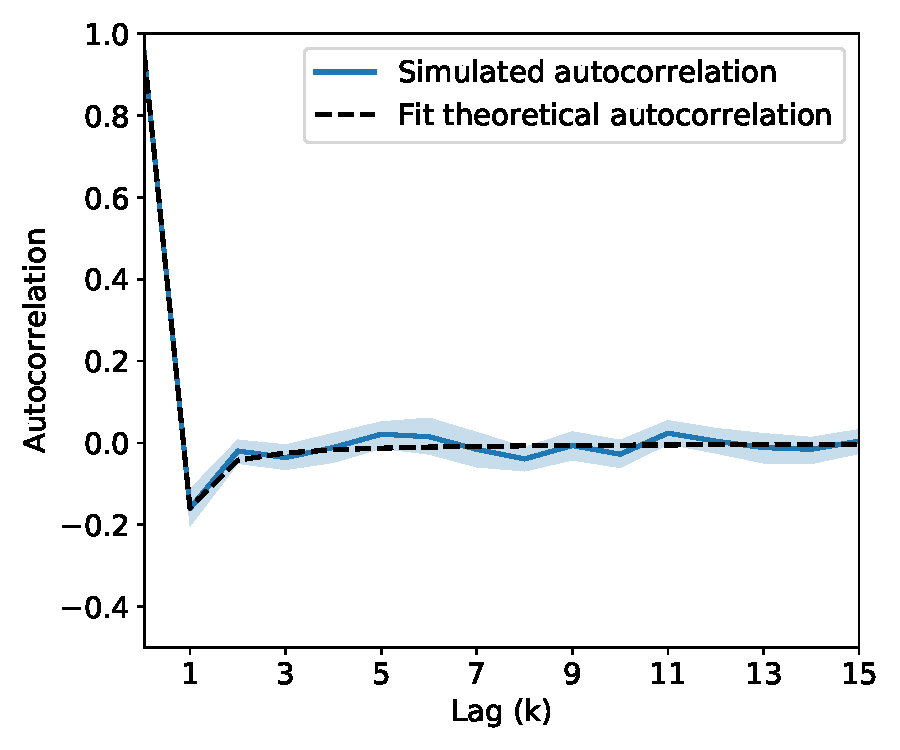
\includegraphics[width=\textwidth]{URE_hop_acf.pdf}
  \caption{}\label{fig:hop_acf}
  \end{subfigure}
  \caption{(a) Urea exhibits hops between periods of entrapment, characteristic of a CTRW. 
  (b) The distribution of hop lengths fits well to a Gaussian as well as a more general L\'evy 
  stable distribution. The L\'evy stable distribution does a better job of capturing the 
  heavier tails and increased density near 0. (c) The distribution of dwell times is fit
  well by a power law but it may over-estimate the probability density at long dwell times.
  A power law truncated with an exponential cut-off may better describe the probability of
  long dwell times in our simulations. (d) The hops are negatively correlated to their previous
  hop. In combination, (a) -- (d) support modeling solutes as subordinated fractional Brownian
  and L\'evy motion. The behavior shown by urea in this figure is common to all solutes in this study (see
  Figures~\ref{S-fig:GCL_anticorrelated_hops}--\ref{S-fig:MET_anticorrelated_hops} of the
  Supporting Information).}\label{fig:anticorrelated_hops}
  %MRS4: are there similar figures in the supporting information.
  %BJC4: added
  %MRS6: I'm wondering if the other plots should be in the main text.  They are part of the core of the paper, showing that the modeling is reasonable. 
  \end{figure}
  
  We modeled the distributions of hop lengths in two ways. First, we assumed the 
  distribution to be Gaussian since it is possible to exactly simulate realizations of
  fractional Brownian motion. Second, we fit the distributions to L\'evy stable 
  distributions since it is more general than the Gaussian distribution. We plotted
  the MLE fits of both on top of urea's hop length distribution in 
  Figure~\ref{fig:hop_distribution_comparison}. The L\'evy distribution does a better
  job capturing the somewhat heavy tails and high density near 0 of the hop length distribution.
  However, since there are no known exact simulation techniques for generating 
  realizations of fractional L\'evy motion, we must evaluate whether this more general
  fit is worthwhile. 
  
  We also modeled the distribution of dwell times in two ways. First, we assumed pure
  power law behavior since it is consistent with most theoretical descriptions of CTRWs.
  The data fits well to this model at short dwell times but the density of long dwell
  times is over-estimated. In our second approach, we truncate the power law distribution
  with an exponential cut-off, lowering the probability of extremely long dwell times. 
  We demonstrate this effect in the inset to Figure~\ref{fig:powerlaw}, where the
  density of the truncated power law drops below that of the pure power law and tends towards
  0 near a dwell time of 250 ns.
  
  Realizations of the AD model based on the parameterization procedures just described
  yield qualitatively similar trajectories to those seen in our MD simulations. In
  Figure~\ref{fig:ad_eyetest}, we plot representative sample trajectories for each
  combination of the dwell time and hop distribution, labeled according to Table~\ref{table:anomalous_models}.
  The sFBMcut and sFLMcut in particular resemble the trajectories in Figure~\ref{fig:solute_trajectories}.
  When we do not truncate the dwell time distribution, the trajectories tend to 
  incorporate very long dwell times as shown by the sFBM and sFLM models.
  
  \begin{figure}
  \centering
  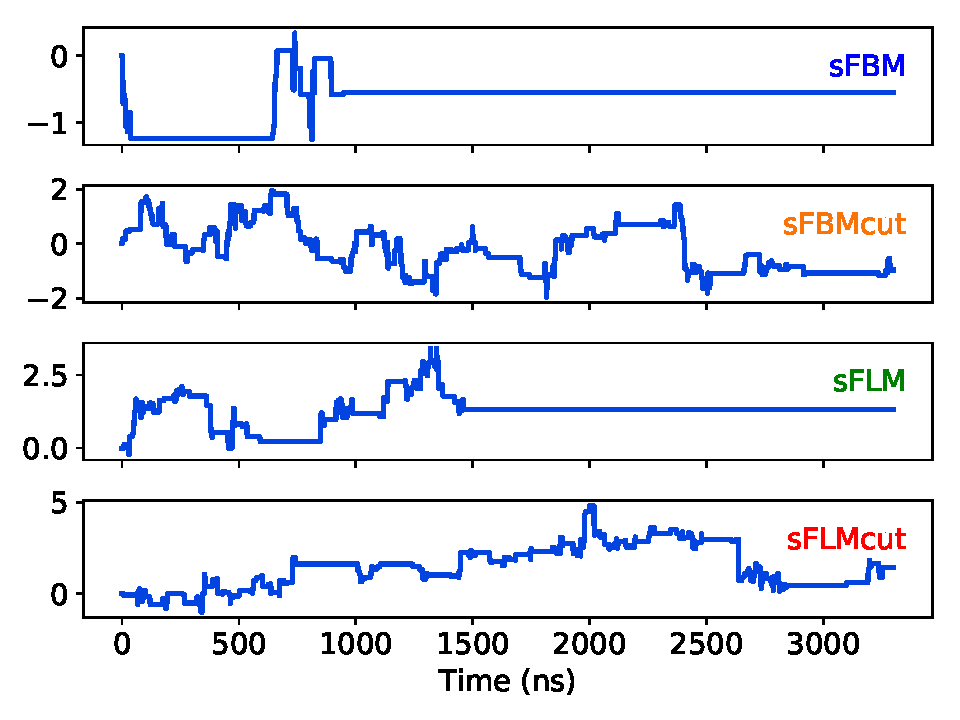
\includegraphics[width=0.5\textwidth]{ad_realizations_1mode.pdf}
  \caption{Simulations of 1 mode AD model trajectories for urea display qualitatively
  similar hopping and trapping behavior to that shown in Figure~\ref{fig:solute_trajectories}. 
  Dwell times appear exaggerated in the sFBM and sFLM models because the power law dwell
  time distributions are not truncated and have infinite variance.
  %Analogous plots are shown for other solutes
  %MRS6: I don't think the comparison between the cut and no cut are that interesting for the main text.  Move to supporting?
  %MRS6: comparisons between modeled and actual trajectories side by side would be more interesting. 
  %BJC5: todo: add plots to SI. Show I add a 2 mode model plot?
  %and the 2 mode model in the Supporting Information. 
  }\label{fig:ad_eyetest}
  \end{figure}
  
  \subsubsection{Model validation on stationary trajectories}\label{section:sfbm_validation}

  We evaluated the predictive capabilities of the AD modeling approach by training
  the model parameters on the first half of the equilibrated MD trajectory data and
  then comparing the MSD calculated from AD model realizations to the MSD calculated
  from the second half of the equilibrated MD trajectory data. This metric is
  only meaningful if the ensemble of solute trajectories is stationary.
  
  We observe that in many cases, the distribution of solutes within the membrane
  evolves slowly with time. We defined the perceived equilibration time point 
  for each solute based on the time at which the number of solutes inside the
  pores and tails stabilized (Figure~\ref{S-fig:equilibration}). Nonetheless, we observe evidence of non-stationary
  solute behavior after equilibration, on the $\mu$s timescale. In Table~\ref{table:stationarity},
  we compare the MSD of the solutes calculated using trajectory data from the 
  first and second halves of the ``equilibrated" simulation time. Ethylene glycol 
  and methanol show considerable differences in their MSDs. Urea and acetic acid
  appear to demonstrate satisfactory stationarity. The shapes of their MSDs curves
  are also very similar (see Figure~\ref{S-fig:msd_comparison} of the Supporting
  Information).
  
  \begin{table}[h]
  \centering
  \begin{tabular}{|c|c|c|}
  \hline
  \multirow{2}{*}{Residue} & \multicolumn{2}{c|}{MSD}            \\\cline{2-3}
                           & First Half       & Second Half      \\\hline
  Urea                     & 0.31 (0.23, 0.40)& 0.35 (0.28, 0.43)\\\hline
  Ethylene Glycol          & 3.11 (2.06, 4.25)& 1.03 (0.76, 1.29)\\\hline
  Methanol                 & 2.24 (1.61, 2.92)& 1.06 (0.77, 1.39)\\\hline
  Acetic Acid              & 1.58 (1.11, 2.03)& 1.43 (1.10, 1.73)\\\hline

  %MRS6: you don't say what is in the paragraphs.
  \end{tabular}
  \caption{In order to be considered stationary, the MSD of the ensemble of solute trajectories
  should be the same independent of the portion of equilibrated trajectory that is
  analyzed. The MSD values in this table are averages taken after a 500 ns time lag, 
  calculated independently from the first and second halves of the equilibrated
  solute trajectories. Urea and acetic acid both appear to satisfy the stationarity
  criteria, while ethylene glycol and methanol show significantly smaller MSDs 
  when calculated from the second half of the equilibrated trajectories.}\label{table:stationarity}
  \end{table}
  
%  The non-stationary behavior of ethylene glycol and methanol present themselves
%  in different ways. On average, methanol molecules in the tails appear to be 
%  drifting further away from the pore center with time. Methanol's small size 
%  significantly increases the volume of accessible structural space. Ethylene 
%  glycol appears to experience an increased incidence of long trapping times. 
%  These problems probably cannot be addressed without more simulation time or 
%  additional solute trajectories. 

  Using the approach described above, we validated our 1 and 2 mode models with
  urea and acetic acid, since their trajectories appear stationary. 
  The MSDs resulting from 1000 realizations of the AD model are shown in 
  Figure~\ref{fig:train_test}. We consider the model's prediction to match well if the
  MSD lies within the 1$\sigma$ confidence intervals of the MD MSDs. We also
  look for qualitative agreement in the shape of the curves.
  
  \begin{figure}
  \centering
  \begin{subfigure}{0.45\textwidth}
  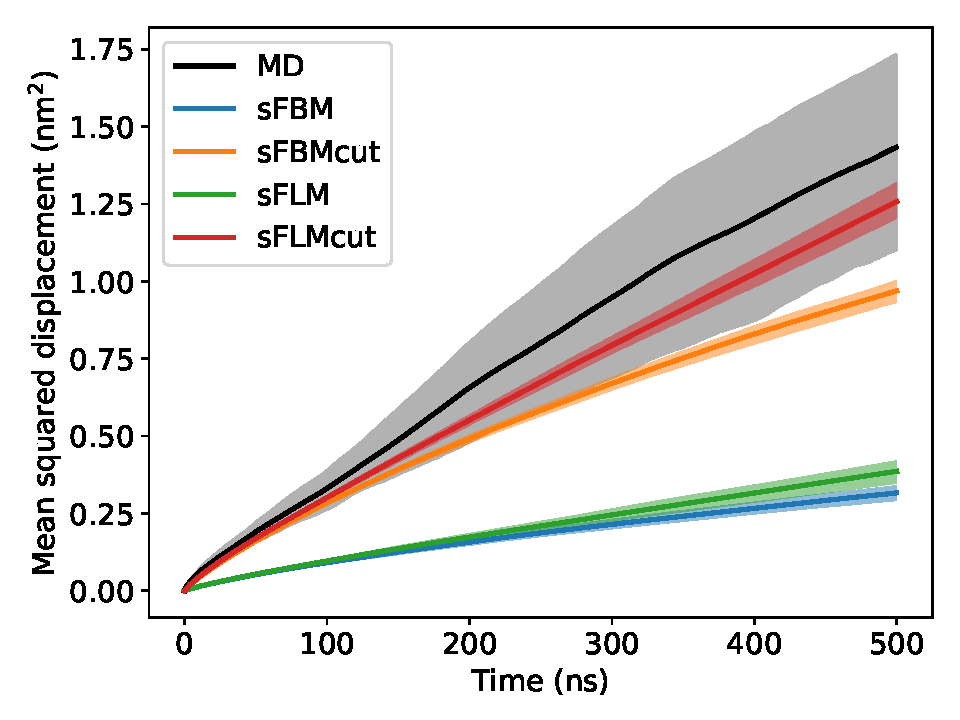
\includegraphics[width=\textwidth]{1mode_msd_comparison_URE_train_front.pdf}
  \caption{Urea (1 mode)}\label{fig:1mode_msd_comparison_URE_train_front}
  \end{subfigure}
  \begin{subfigure}{0.45\textwidth}
  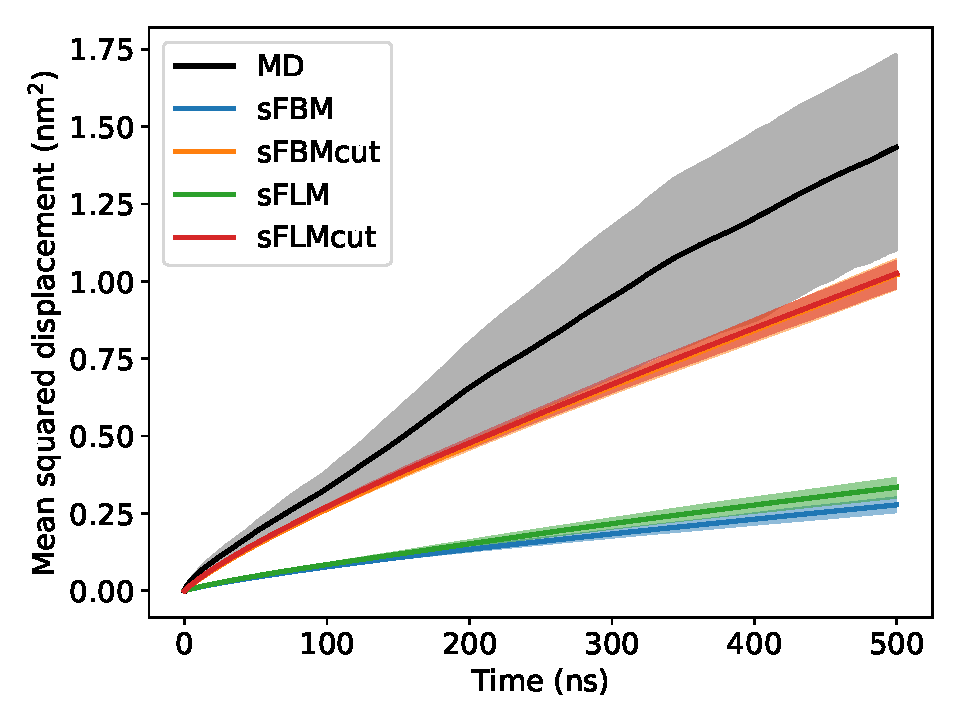
\includegraphics[width=\textwidth]{2mode_msd_comparison_URE_train_front.pdf}
  \caption{Urea (2 modes)}\label{fig:2mode_msd_comparison_URE_train_front}
  \end{subfigure}
  \begin{subfigure}{0.45\textwidth}
  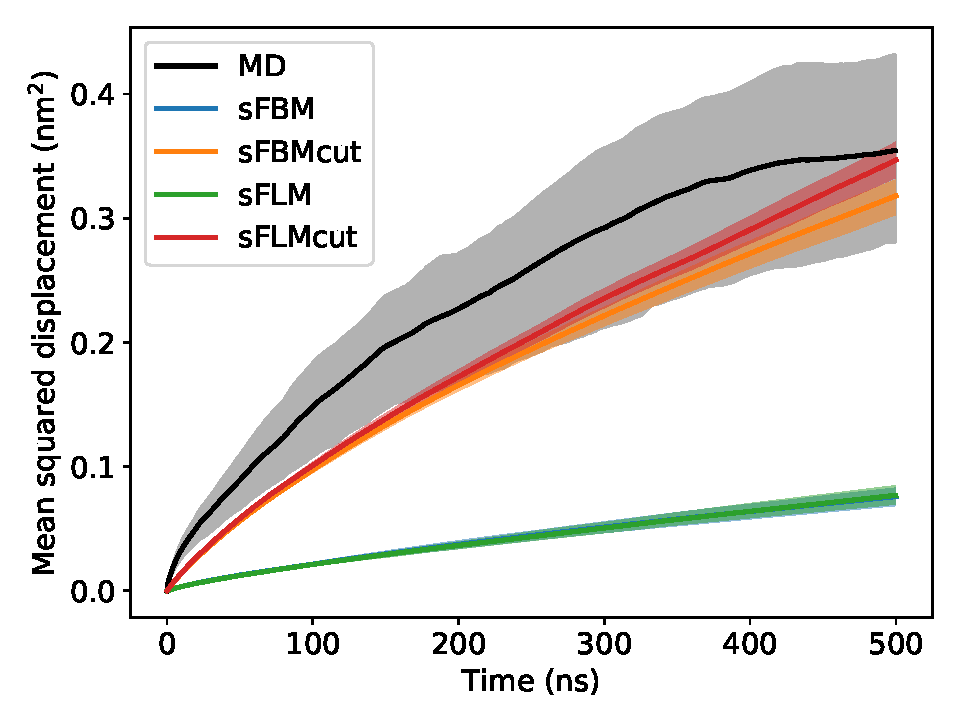
\includegraphics[width=\textwidth]{1mode_msd_comparison_ACH_train_front.pdf}
  \caption{Acetic acid (1 mode)}\label{fig:1mode_msd_comparison_ACH_train_front}
  \end{subfigure}
  \begin{subfigure}{0.45\textwidth}
  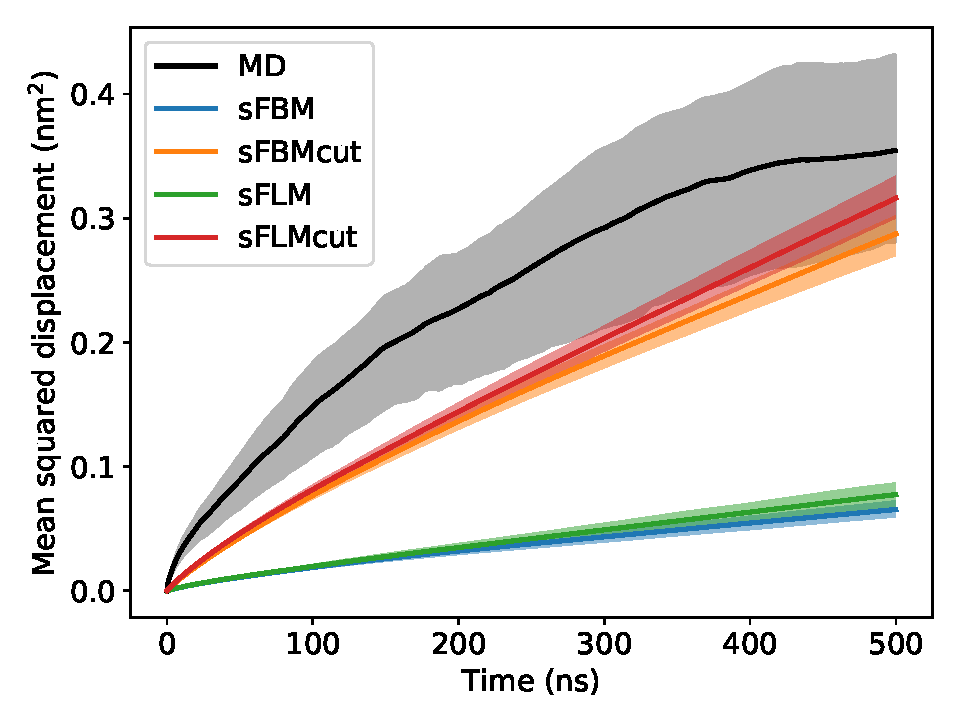
\includegraphics[width=\textwidth]{2mode_msd_comparison_ACH_train_front.pdf}
  \caption{Acetic acid (2 modes)}\label{fig:2mode_msd_comparison_ACH_train_front}
  \end{subfigure} 
  %MRS6: I'm not sure I see red in urea.  Is the uncertainty that low?
  \caption{In most cases, when using power laws with exponential cut-offs 
  (sFBMcut and sFLMcut), the MSD curves predicted by the AD model trained on 
  the first half of the equilibrated data lie within the 1$\sigma$ confidence
  intervals of the MD MSD curves generated from the second half of the equilibrated
  solute data. The models which use pure power laws systematically under-predict
  the MD MSD curves. 
  %MRS6: be more specific when you say ``improper''. What is improper?
Improper curvature of the MSD curves cause the magnitude of
  the urea's predicted MSDs to be under-predicted at long timescales and those
  of acetic acid to be under-predicted at short timescales.}\label{fig:train_test}
  %MRS6: I'm not sure it makes sense to show the ``without cutoff'' lines here.  Maybe supporting?  
  %MRS6: I'm just not sure it really pushes the paper forward to show more data that something you've shown
  %MRS6: isn't likely to work earlier still isn't working. 
  \end{figure}
  
  The models are capable of reasonably predicting the MD MSD values of the second
  half of the solute trajectories based on parameters generated from the first half
  when the dwell time distributions are parameterized by a power law with an 
  exponential cut-off. At long timescales, the MSD of Urea is under-predicted 
  for both the 1 and 2 mode models with the same true of acetic acid on short 
  timescales. Without truncation of the power law distribution, the MD 
  MSDs are underestimated in all cases because dwell times on the order of the
  MD simulation length are sampled and incorporated into the simulated anomalous
  diffusion trajectories. Considering the longest observed dwell time among all
  solutes was 1.3 $\mu$s by ethylene glycol, we believe truncation is well-justified.
  %Although in most cases, the predicted MSD curves overlap the 1-$\sigma$ confidence
  %intervals of the MD MSD curves, they appear to lie systematically below the mean. 
  %It is not clear whether this is a consistent feature of the AD model since we 
  %only used 2 solutes for this analysis. 
  
%  We also observe that simulated AD trajectories which draw from a L\'evy stable 
%  distribution generally predict higher MSDs. The heavy tails of the distribution 
%  incorporate large jumps more frequently into the trajectories. 
  
  From a qualitative perspective, the models only have moderate success at predicting
  the shape of the MSD curves. Error in the MSD curvature can also help explain some of
  the error in the predicted MSD magnitudes. The curves predicted for Urea with both 1 
  and 2 modes appear to have too much curvature, which causes it to under-predict the 
  MSD at long timescales, while those of acetic acid lack curvature, leading the
  AD model to under-predict the MSD at short timescales. 
  
  The under-estimate of Urea's MSD at long timescales is due to long timescale
  positional anti-correlation which may not be present in the 
  %MRS6: real?
  %real 
  molecularly detailed simulations of the 
  system. The 
  %MRS6: I'm not following whether or not there should be positional anti-correlation.  I was thinking there should be,
  %but perhaps I'm misunderstanding something here? 
  persistent curvature of the predicted MSD curves is a direct consequence of 
  the Hurst parameter. Without anti-correlation, the process would be 
  a pure CTRW for which one would expect the time averaged MSD curves to become 
  linear.~\cite{meroz_toolbox_2015} It may be true that on the $\mu$s time scale, 
  positional correlation is lost which would manifest as a transition from a sub-linear
  to linear MSD curve. A solution for more accurately modeling this behavior in  
  the future may be to truncate the positional autocorrelation function.~\cite{molina-garcia_crossover_2018}
  
  The under-estimate of the curvature of acetic acid's predicted MSD suggests that,
  in this case, the AD model over-estimates the Hurst parameter. This is not surprising
  because the Hurst parameter is challenging to quantify, especially with a relatively 
  small amount of data (see Section~\ref{method:sfbm} for further discussion of this 
  challenge). A more accurate measurement of $H$ would fix the shape of the MSD curve,
  but also lower the predicted MSD meaning we are either underestimating the width of
  the hop length distribution, favoring longer dwell times, or both.
  
%  Urea's curves appear to have
%  close to the right amount of curvature at short timescales 
  
%  In general, the MSDs generated by our AD models appear
%  close to linear at long time scales. This is expected behavior for time averaged 
%  MSDs, especially when truncating the power law distribution of dwell times.
%  \cite{molina-garcia_crossover_2018} The linearity of Urea's MD MSD curve is 
%  consistent with that of the AD model, but the MD MSD of acetic acid appears to have considerable
%  curvature. 
  
%  Acetic acid's MSD is under-predicted at short timescales but within error 
%  of MD (using sFBMcut and sFLMcut models) after a 500 ns time lag. The curvature suggests that the 
%  model under-estimates long timescale positional anti-correlation which points to an
%  over-estimate of the Hurst parameter. This is not surprising because the Hurst 
%  parameter is challenging to quantify, especially with a relatively small amount of 
%  data (see Section~\ref{method:sfbm} for further discussion of this challenge).
%  A more accurate measurement of $H$ would fix the shape of the MSD curve, but also
%  lower the predicted MSD meaning we are either underestimating the width of the hop
%  length distribution, favoring longer dwell times or both.
  % BJC4: play around with this to see how to change shape of acetic acid curve. Hurst makes it arc more
  % ctrwsim.py -alpha 0.08 -fix_time -hop fbm -H 0.34 -ntraj 100 -dwell powerlaw_cutoff -lamb 0.0033 -hs 0.27
  
  This brief qualitative analysis suggests two shortcomings of the AD model. First, in
  a real system, positional anti-correlation may dissipate after a sufficiently long 
  time lag, dependent on the solute being studied. Second, it is difficult to reliably
  parameterize the Hurst parameter which is important for accurately describing the 
  curvature of the solute MSDs.
  
  This analysis also suggests that working with only half of the data we collected
  ($\sim$ 2 $\mu$s post-equilibration) is not always sufficient for extracting reliable
  parameter estimates. In most cases, the magnitude of the MSD predictions after a 
  500 ns time lag are within or close to within error of the MD MSDs (for sFBMcut and
  sFLMcut), but still appear to systematically under-predict the mean. We may be
  operating on the border of the minimum amount of data required to accurately 
  parameterize the AD model. Longer simulations and more independent trajectories may
  be necessary. Therefore, in the next section we will work with parameters fit to the
  full equilibrated portion of the solute trajectories, doubling the data.
  
%MRS6: My instinct is to only show the graphs of the full model, with validation graphs shown in the supporting.  We can talk about this. We do what the focus to be on what we can learn physically.  The discussion gets pretty repetitive.
  
%MRS6: be a bit clearer about how the MD MSD error bounds are calculated.  That becomes important for determining how accurate the modeling is. . 

%  However, in the case of acetic acid, this may only happen because the 
%  Hurst parameter is overestimated. It appears we are operating on the border of the
%  minimum amount of data required to accurately parameterize the AD model. Longer
%  simulations and more independent trajectories may be necessary. Therefore, in 
%  the next section we will work with parameters fit to the full equilibrated portion
%  of the solute trajectories, doubling the data.

%  This brief analysis highlights some of the shortcomings of the AD model. So far, we have 
%  shown that it does a reasonable job of approximating the magnitude of the MD-MSD
%  after a 500 ns time lag, but the shape can sometimes be qualitatively wrong because of
%  inaccurate Hurst parameters. In the case of acetic acid, a poorly measured $H$, but 
%  accurate prediction of the magnitude of the MSD after 500 ns, may mask underlying 
%  problems with the parameters of the hop length and dwell time distributions. Acetic
%  acid has the lowest MSD of the solutes studied, therefore these issues may be resolved
%  by longer simulations.
 
  %BJC4: comment here about the length of time simulations need to be run in 
  % order to get reliable data
  % Or maybe a little later since acetic acid, although stationary
  % comment on acetic acid's trajectory shape.
  
  \subsubsection{Model predictions using all equilibrated data}\label{section:AD_all_data}
  
  We obtain reasonable predictions of the MD simulated MSDs when we parameterize the AD 
  model with all available data after the perceived equilibration time. Although we 
  concluded that methanol and ethylene glycol trajectories are not yet stationary, we 
  include them in all analysis going forward because it is still instructive. 
  The MSD curves generated from 1 and 2 mode models are overlayed with the MD simulated MSDs for 
  comparison in Figures~\ref{fig:anomalous_msds_1mode} and~\ref{fig:anomalous_msds_2mode}
  respectively. The associated parameters are presented in Figures~\ref{fig:1mode_parameters}
  and~\ref{fig:2mode_parameters}.
  
  \begin{figure}
  \centering
  \begin{subfigure}{0.45\textwidth}
  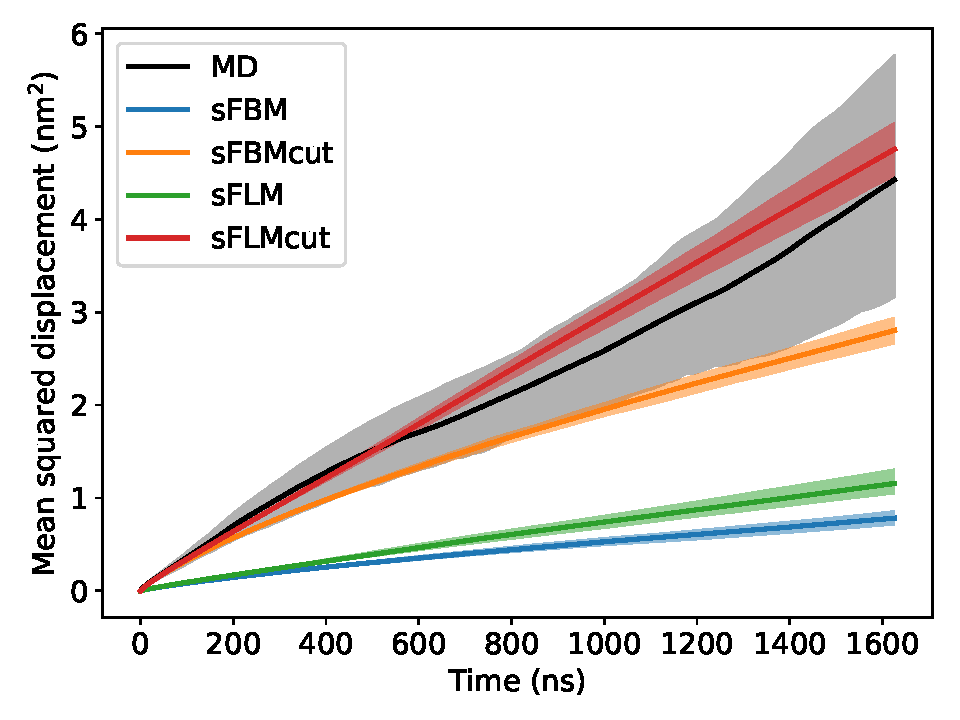
\includegraphics[width=\textwidth]{1mode_msd_comparison_URE.pdf}
  \caption{Urea}\label{fig:1mode_msd_comparison_URE}
  \end{subfigure}
  \begin{subfigure}{0.45\textwidth}
  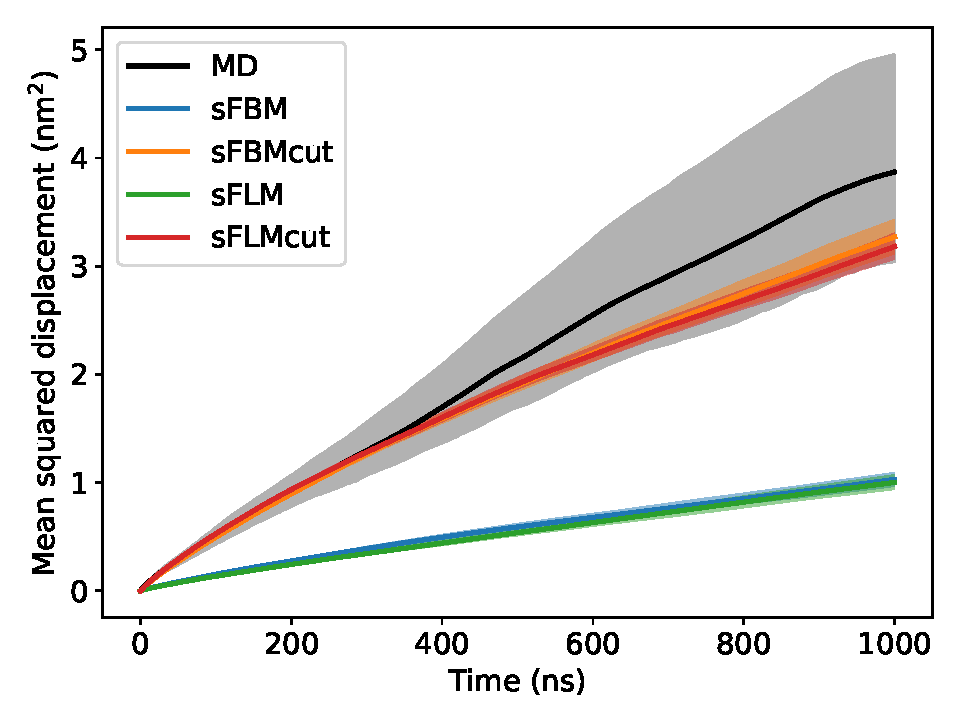
\includegraphics[width=\textwidth]{1mode_msd_comparison_GCL.pdf}
  \caption{Ethylene Glycol}\label{fig:1mode_msd_comparison_GCL}
  \end{subfigure}
  \begin{subfigure}{0.45\textwidth}
  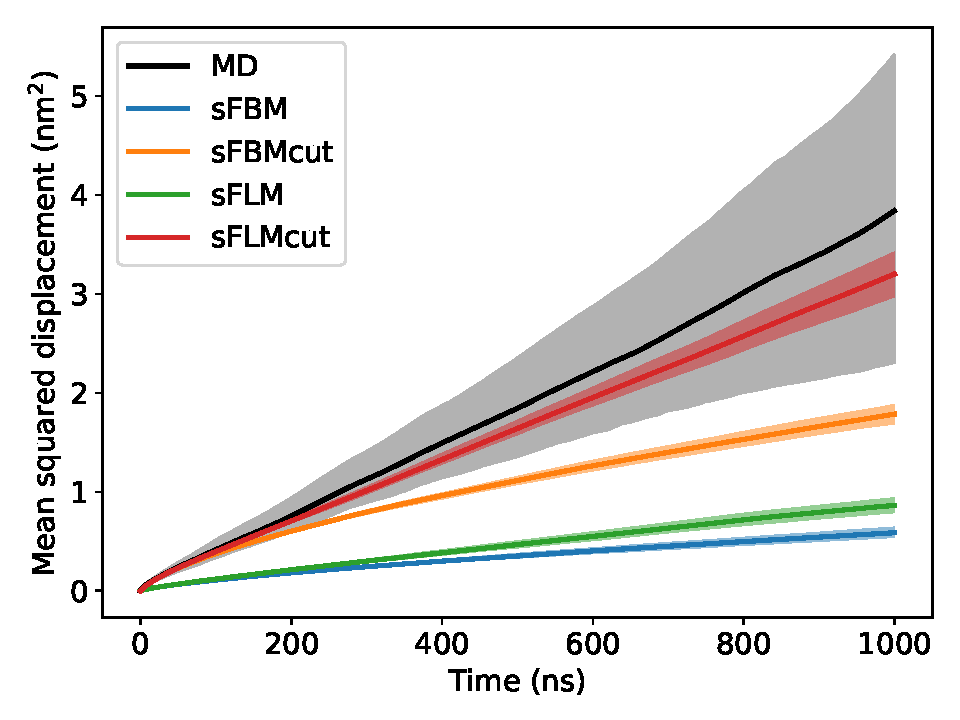
\includegraphics[width=\textwidth]{1mode_msd_comparison_MET.pdf}
  \caption{Methanol}\label{fig:1mode_msd_comparison_MET}
  \end{subfigure}
  \begin{subfigure}{0.45\textwidth}
  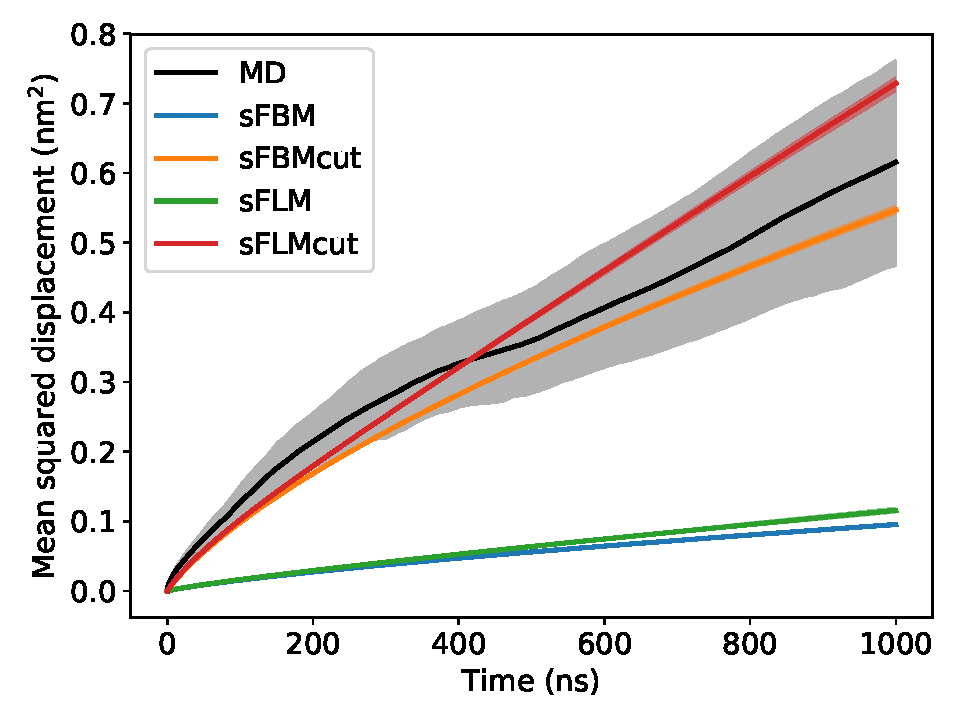
\includegraphics[width=\textwidth]{1mode_msd_comparison_ACH.pdf}
  \caption{Acetic Acid}\label{fig:1mode_msd_comparison_ACH}
  \end{subfigure}
  \caption{In most cases, MSDs generated from realizations of our 1 mode anomalous
  lie within or near the 1$\sigma$ confidence intervals of MD-generated data when using an
  exponential cutoff on the dwell time distribution (sFBMcut and SFLMcut). When we
  do not apply an exponential cut-off (sFBM and SFLM), MSDs are underpredicted. 
  Drawing hops from a truncated L\'evy stable distribution yields MSDs similar to 
  when hops are drawn from Gaussian disributions (sFLM and sFLMcut). In most 
  cases, the MSDs are under-predicted at long timescales because the AD models
  show pronounced curvature which the MD simulations lack.}\label{fig:anomalous_msds_1mode}
  \end{figure}
  
  \begin{figure}
  \centering
  \begin{subfigure}{0.45\textwidth}
  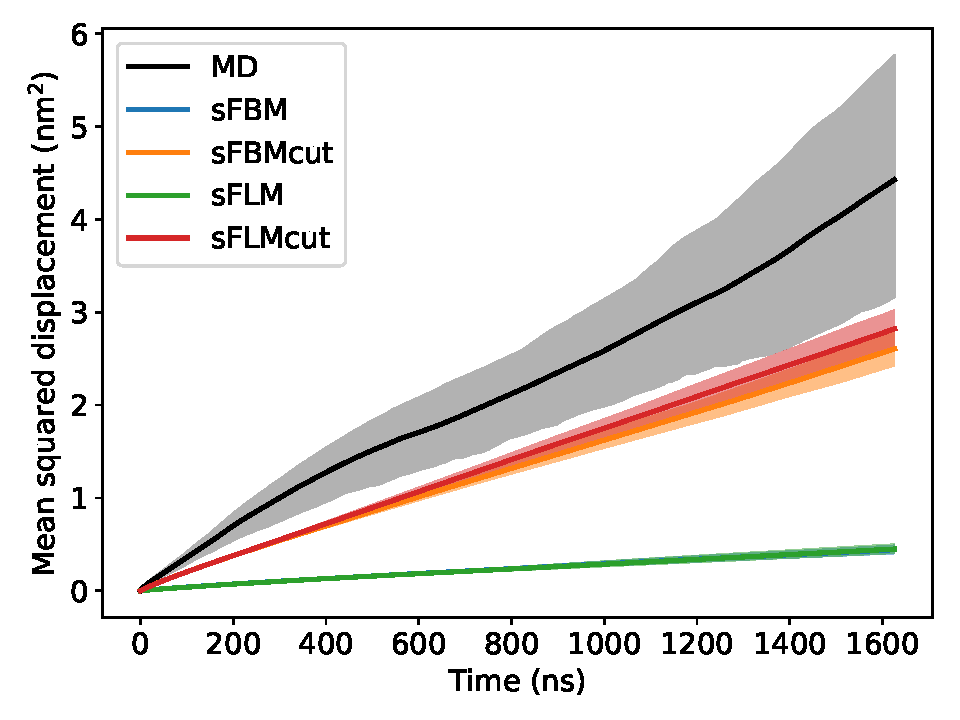
\includegraphics[width=\textwidth]{2mode_msd_comparison_URE.pdf}
  \caption{Urea}\label{fig:2mode_msd_comparison_URE}
  \end{subfigure}
  \begin{subfigure}{0.45\textwidth}
  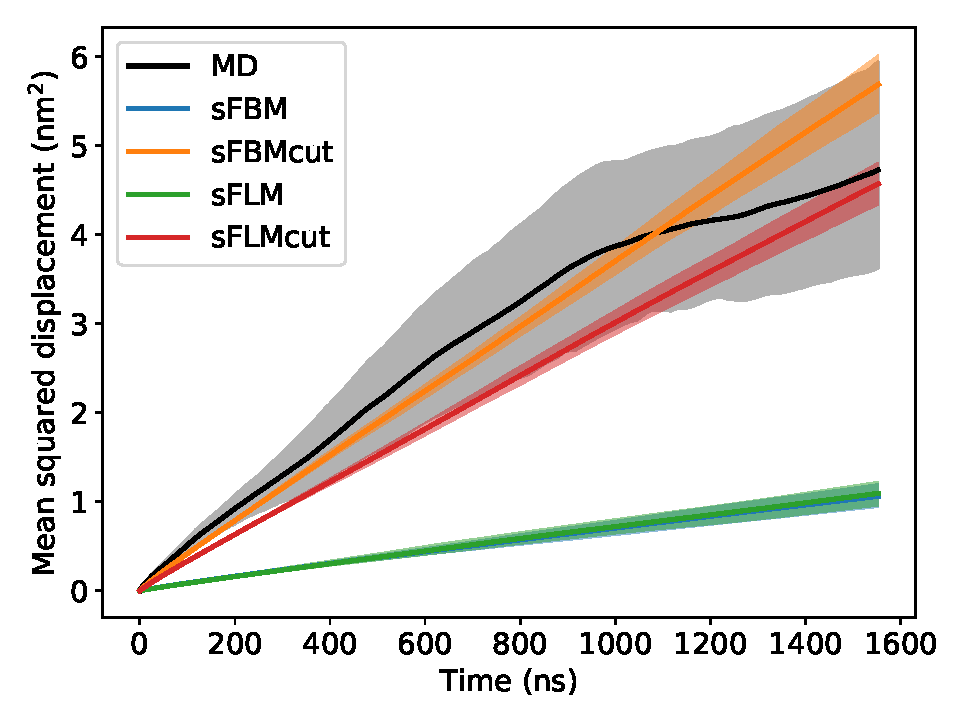
\includegraphics[width=\textwidth]{2mode_msd_comparison_GCL.pdf}
  \caption{Ethylene Glycol}\label{fig:2mode_msd_comparison_GCL}
  \end{subfigure}
  \begin{subfigure}{0.45\textwidth}
  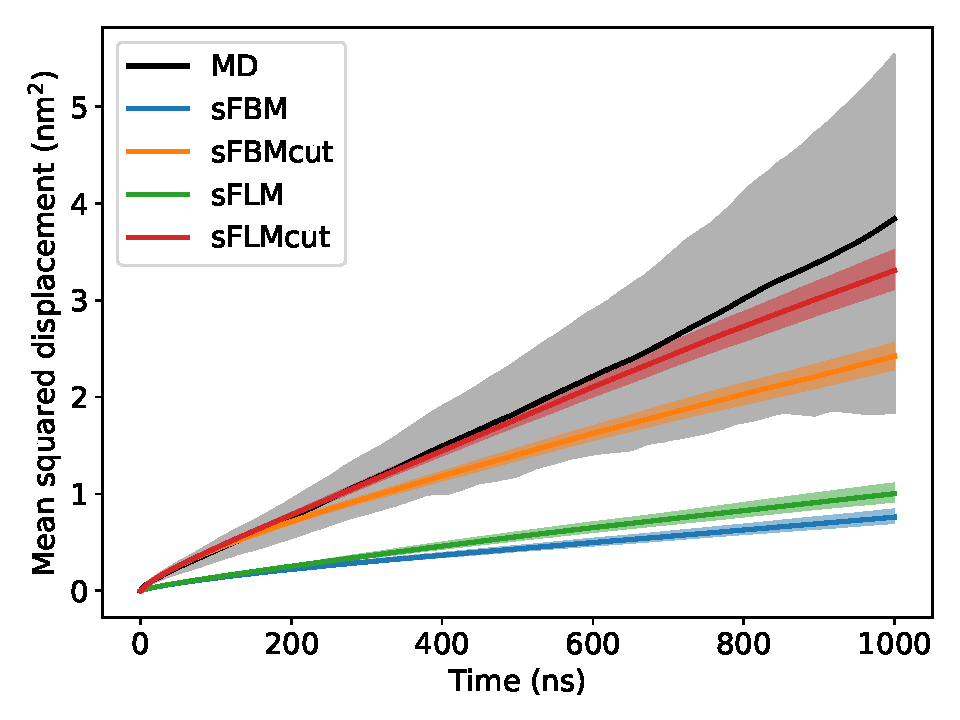
\includegraphics[width=\textwidth]{2mode_msd_comparison_MET.pdf}
  \caption{Methanol}\label{fig:2mode_msd_comparison_MET}
  \end{subfigure}
  \begin{subfigure}{0.45\textwidth}
  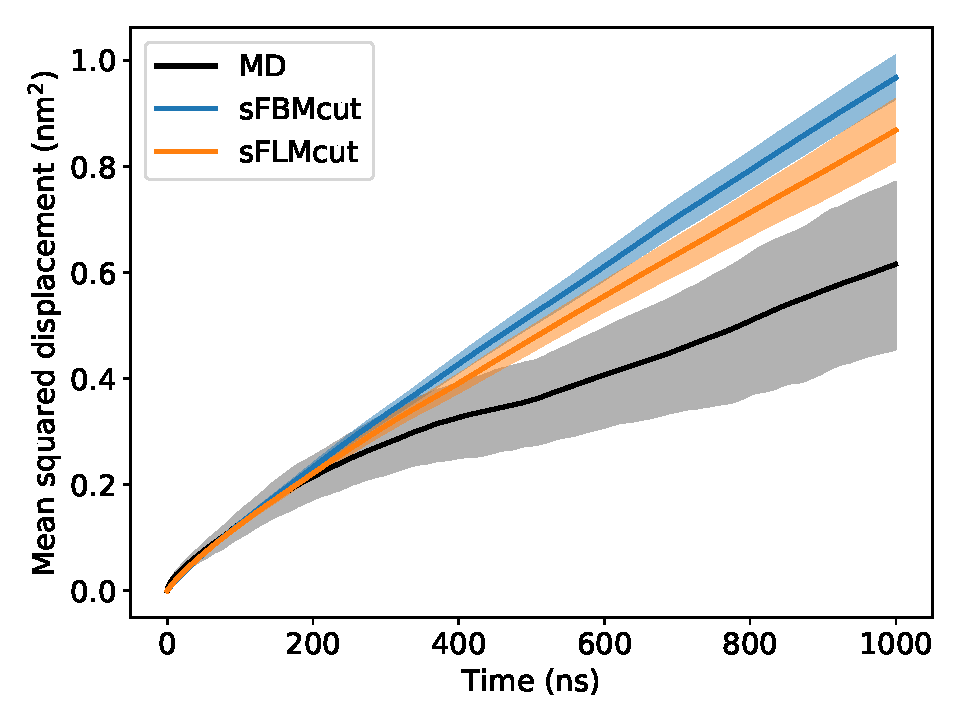
\includegraphics[width=\textwidth]{2mode_msd_comparison_ACH.pdf}
  \caption{Acetic Acid}\label{fig:2mode_msd_comparison_ACH}
  \end{subfigure}
  \caption{MSDs generated from realizations of our 2-mode anomalous diffusion model
  predict the magnitude of the MSDs to a similar degree of accuracy as the 1 mode
  model. Relative to the predictions of the 1 mode model the MSDs lack curvature because
  the hop correlation structure is broken every time a transition between tails occurs.}\label{fig:anomalous_msds_2mode}
  \end{figure}
  
  \begin{figure}
  \centering
  \begin{subfigure}{0.325\textwidth}
  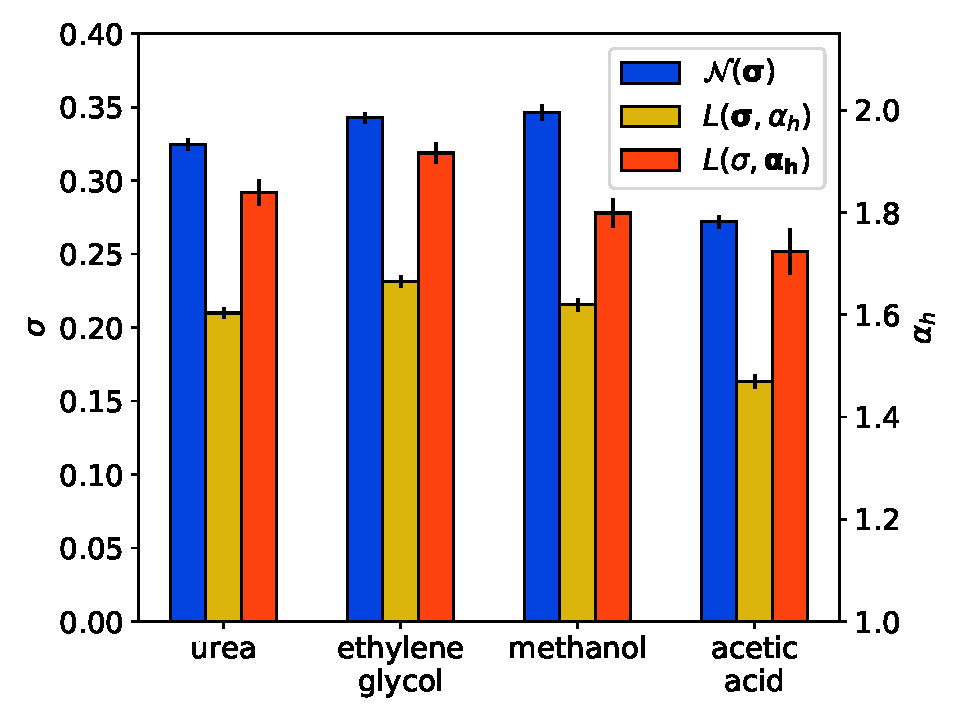
\includegraphics[width=\textwidth]{1mode_AD_hops.pdf}
  \caption{}\label{fig:1mode_AD_hops}
  \end{subfigure}
  \begin{subfigure}{0.325\textwidth}
  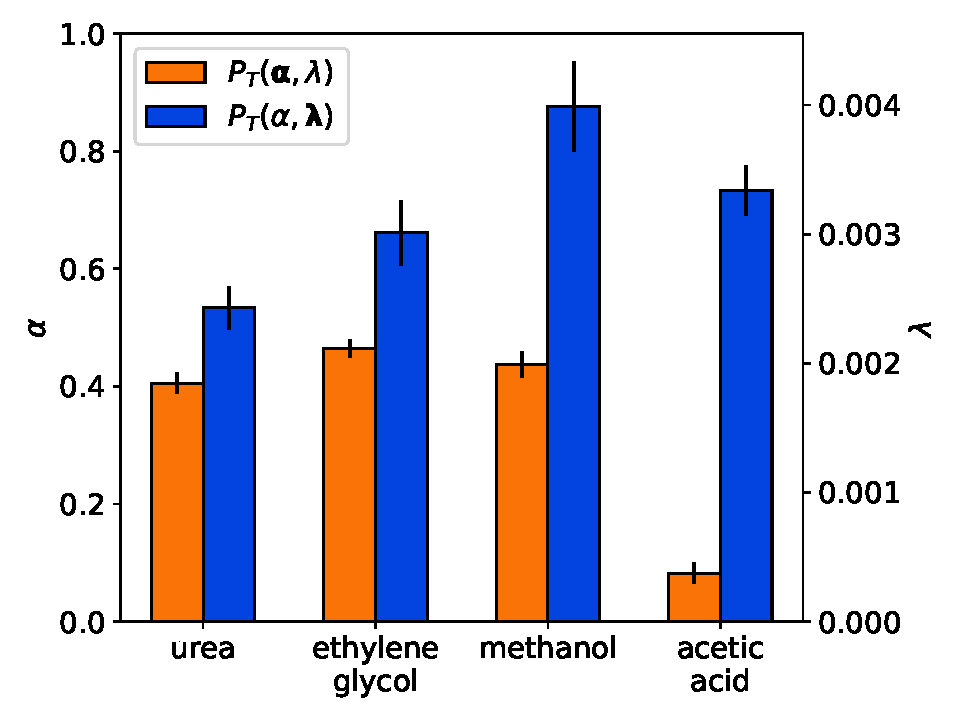
\includegraphics[width=\textwidth]{1mode_AD_dwells.pdf}
  \caption{}\label{fig:1mode_AD_dwells}
  \end{subfigure}
  \begin{subfigure}{0.325\textwidth}
  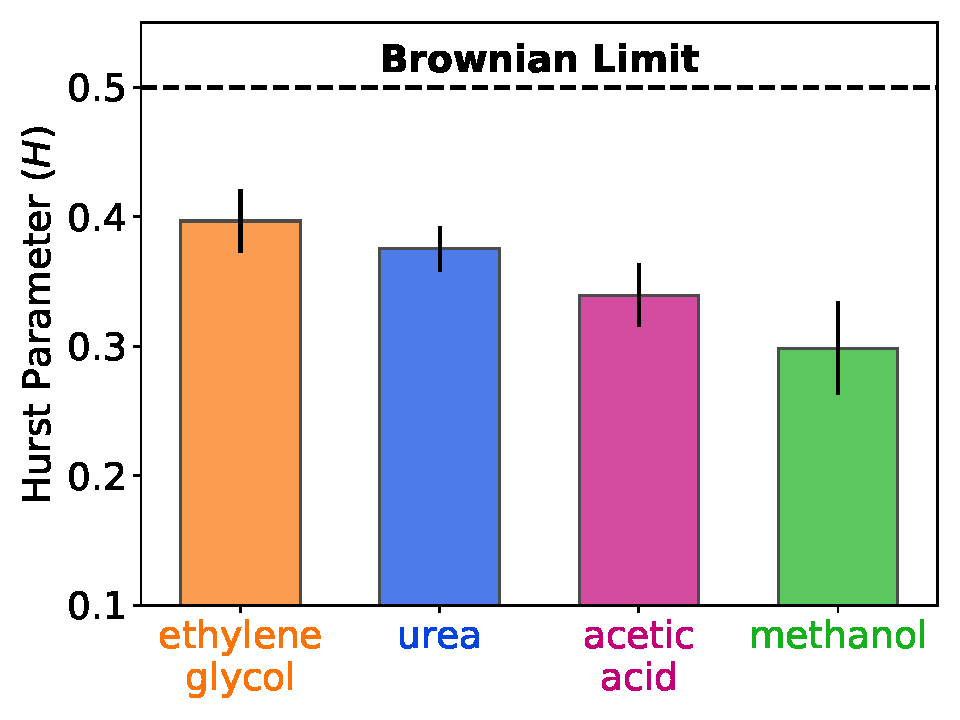
\includegraphics[width=\textwidth]{hurst_barchart.pdf}
  \caption{}\label{fig:hurst_barchart}
  \end{subfigure}
  \caption{The parameters of the 1 mode model reveal differences in solute dynamics.
  (a) We parameterized Gaussian, $\mathcal{N}(\sigma)$, and L\'evy stable, 
  $L(\sigma, \alpha_h)$, distributions to describe solute hop lengths. We assume the 
  mean ($\mu$) to be zero for these distributions and there to be no skewness ($\beta = 0$)
  in the L\'evy stable disributions. High values of $\sigma$ and lower values of $\alpha_h$
  result in larger hops. (b) We parameterized a pure power law, $P(\alpha_d)$, and a 
  truncated power law, $P_T(\alpha_d, \lambda)$, distribution to describe solute dwell
  times. Lower values of $\alpha_d$ lead to heavier power law tails and higher values of 
  $\lambda$ truncate the distibution at lower dwell times. (c) Finally, we parameterized the
  hop autocorrelation function, $\gamma(H)$, to describe the degree of correlation between
  hops. Higher values of $H$ display closer to Brownian behavior.}\label{fig:1mode_parameters}
  \end{figure}
  
  \begin{figure}
  \centering
  \begin{subfigure}{0.475\textwidth}
  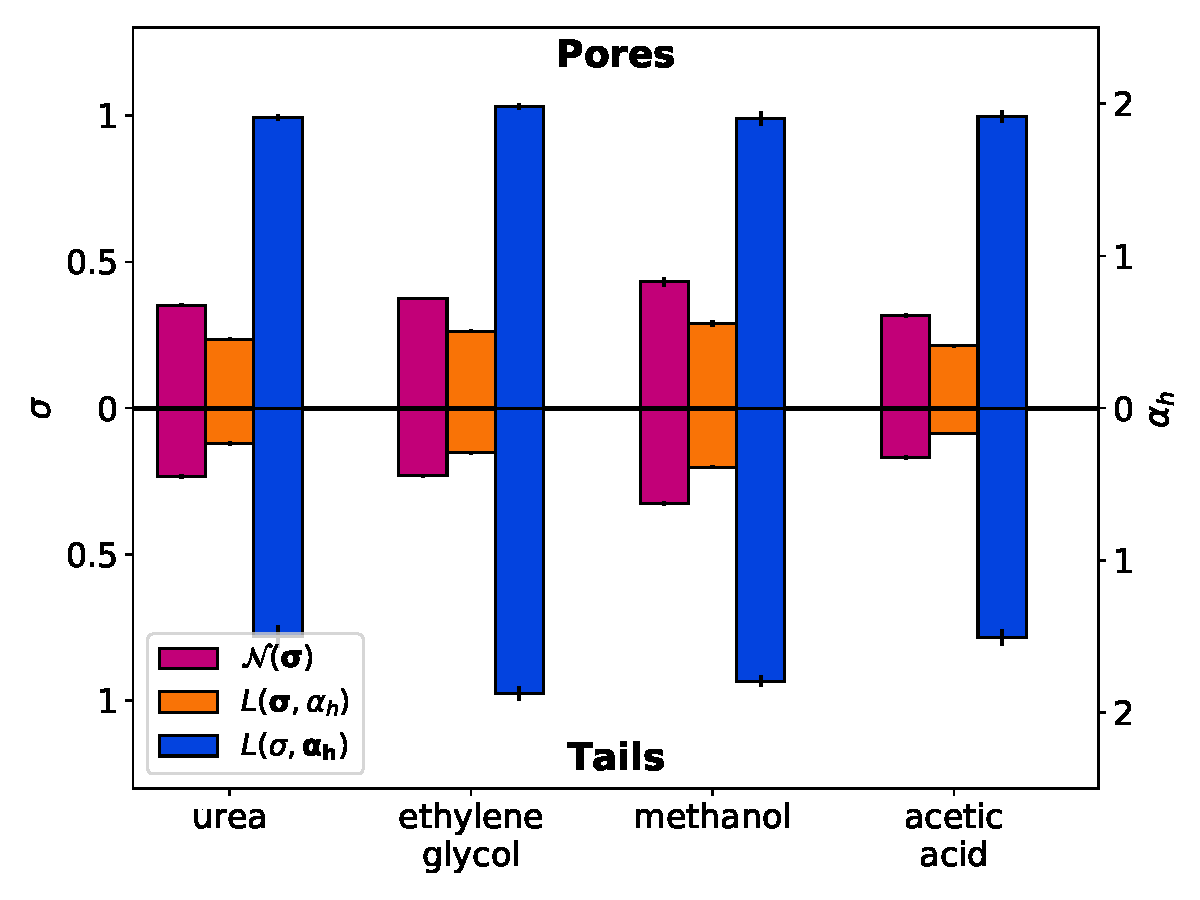
\includegraphics[width=\textwidth]{2mode_AD_hops.pdf}
  \caption{}\label{fig:2mode_AD_hops}
  \end{subfigure}
  \begin{subfigure}{0.475\textwidth}
  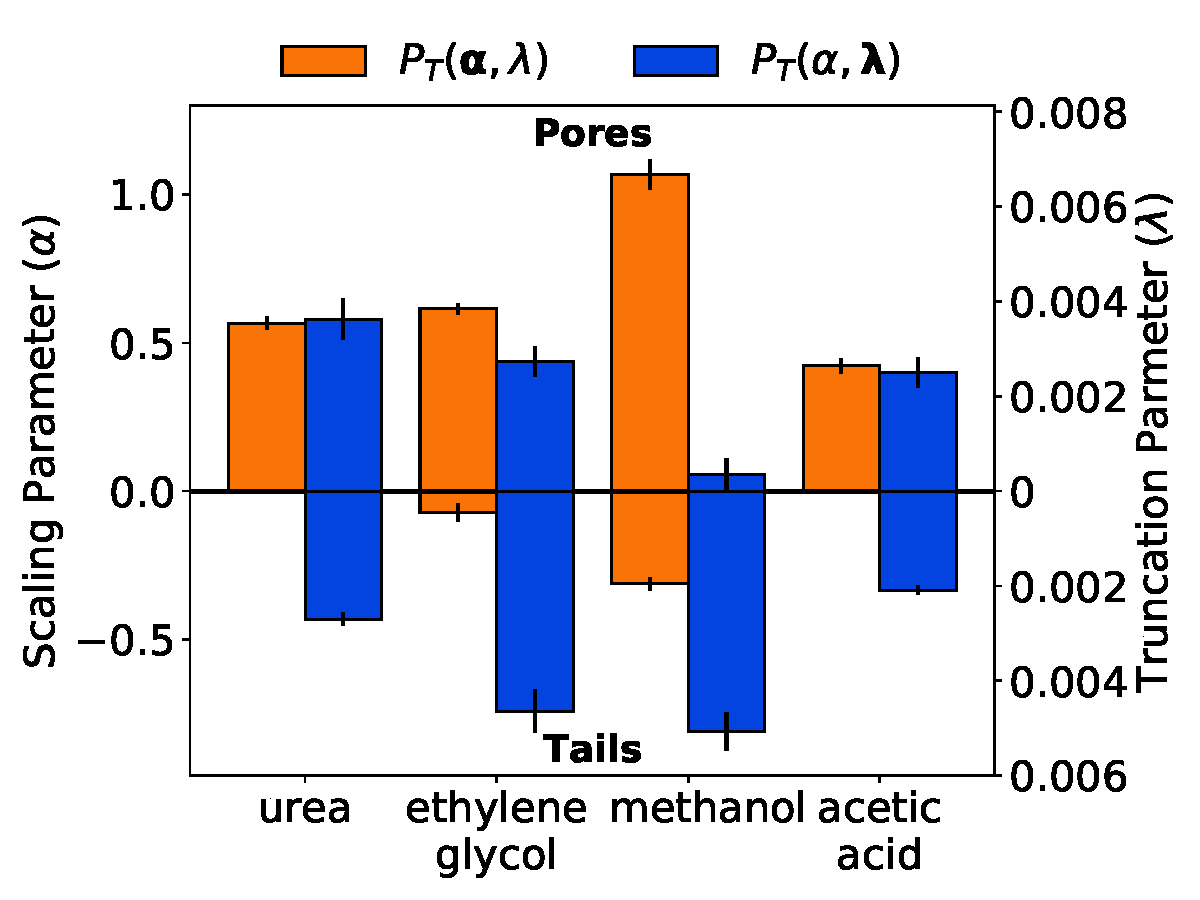
\includegraphics[width=\textwidth]{2mode_AD_dwells.pdf}
  \caption{}\label{fig:2mode_AD_dwells}
  \end{subfigure}
  \caption{
  %MRS6: shouldnt the values be positive below the axis as well (if that can be done) I guess they are for b, but not for A.
  The two mode model parameterizes solute behavior in the pore and tails separately.
  We consider solutes to be within the pore region if they are 0.75 nm from a given pore
  center, otherwise they are in the tails. (a) Generally, movement is much more restricted
  in the tail region shown by lower $\sigma$ 
  %MRS6: define sigma to remind people what it is
  values for the normal and L\'evy stable 
  distributions. Values of $\alpha$ are significantly lower for urea and acetic acid meaning 
  there is a larger probability that they will take large hops. (b) Dwell times are longer in 
  the tails. Lower values of $\alpha_d$ correspond to power laws with heavier tails and 
  thus higher probabilities of long dwell times. There is no easily discernable trend in
  $\lambda$ of the truncated power law distribution. Note that we used the same Hurst parameter
  for both modes (shown in Figure~\ref{fig:hurst_barchart}) due to a low number of 
  sufficiently long sequences of hops in each mode.}
  \label{fig:2mode_parameters}
  \end{figure} 
  
  After a 1000 ns time lag, the 1 and 2 mode AD models do a fairly good job of 
  predicting the magnitude of the MD MSD curves when we use truncated power
  laws to describe the dwell time distributions. In most cases, the sFBMcut
  and sFLMcut models give very similar results probably because their $\alpha_h$
  parameter values are relatively close to 2, meaning the hop length distributions
  are nearly Gaussian even when fit to a more general L\'evy distribution. 
  
  The deviation between the 1 mode MSD predictions and MD are primarily due
  to differences in their curvature at long time lags. The shape and magnitude of the curves appears accurate 
  at short time lags.  
  %MRS6: which curves?
  However, the curves tend to undershoot the MD MSD mean
  as the time lag increases. As discussed in the previous section, long time
  positional anti-correlation may not exist in the MD system which results 
  in a shift from sub-linear to linear MSD behavior. Acetic acid exemplifies
  this point. At first glance, acetic acid's predicted MSD (sFLMcut and sFBMcut)
  appears to match the curvature of MD quite well, but closer examination reveals
  that the MD MSD curve actually shifts from a sub-linear to a linear regime 
  around 500 ns.
  
  %MRS6: is it more or less physical that it has this behavior? 
  The 2 mode models shows considerably less curvature at large time lags than
  the 1 mode model because the implementation of the 2 mode model prevents long
  timescale correlation. The width of the hop distribution changes every time
  a switch between pores and tails occurs. We are unaware of an appropriate
  technique which can correlate hops that come from different hop distributions, 
  therefore every time a mode switch occurs, the correlation structure is 
  broken. Solutes which switch between modes the least show the greatest
  curvature. Methanol spends $> 90\%$ of its time in the tails, so mode transitions
  are relatively rare and the predicted MSD has significant curvature. This artificially
  solves the problem of long timescale correlation, however we do not recommend this
  as it has no theoretical basis.
  
  % In all but one case (two mode 
  % ethylene glycol), MSD curves predicted by the sFLMcut model are higher than 
  % those predicted by the sFBMcut model because of the heavy tails of the L\'evy 
  % stable hop length distribution. 
  
%  Qualitatively, the curves with the highest final MSDs (ethylene glycol and 
%  methanol) show more linear growth and their shapes are well captured by the
%  sFLMcut and sFBMcut AD models. The MSD curve of urea bends slightly and 
%  that of acetic acid has the most significant curvature. When the MD MSD 
%  curves bend, the MSD curves predicted by the sFBMcut model tends to more 
%  accurately portray their curvature since the sFLMcut model tends to become 
%  linear faster.
%  
%  Acetic acid is a notable exception as no model accurately predicts its
%  MSD or curvature. Both sFBMcut and sFLMcut significantly over-predict the final
%  MSD while sFBM and sFLM significantly under-predict it. Once again, it 
%  appears that the Hurst parameter may be over-estimated. However, the parameters
%  of the hop and dwell distributions may be improved over those used to produce
%  Figures~\ref{fig:1mode_msd_comparison_ACH_train_front} and
%  \ref{fig:2mode_msd_comparison_ACH_train_front}. A lower value of $H$ would 
%  increase the curvature and reduce the AD predicted MSD to values more consistent
%  with acetic acid's MD MSD.
  
%  Despite their deviations from the MD, the ranking of the magnitude of predicted
%  MSDs remains the same as MD: ethylene glycol $\approx$ methanol $>$ urea $>$ acetic acid.
%%  The discrepancies between MD and the predictions of the AD model may be resolved
%%  by gathering longer and a greater quantity of solute trajectories
%  Therefore, we can use the current parameters to understand solute dynamics.
  
  The model parameters for the 1 and 2 mode models tell stories about each solute's
  behavior that help explain the difference between the MSDs of different solutes. 
  Higher values of $\sigma$ and lower values of $\alpha_h$ indicate larger average 
  hop length magnitudes by increasing the hop length distribution's width and tail 
  density respectively. Higher values of $\alpha_d$ indicate a lower probability of 
  long dwell times. Higher values of $\lambda$ truncate the power law distribution 
  earlier preventing extremely long dwell times. Values of $H$ closer to the Brownian
  limit of 0.5, indicate a lower degree of negative correlation between hops. All 
  of 
  these model properties
  %which 
  contribute to 
  %MRS6: increase in the MSD compared to what, be specific?
  an overall increase in the MSD.


  Turning first to the parameters of the 1 mode model, we can begin to break down the
  trends in solute MSDs. The parameters belonging to ethylene glycol and methanol are
  relatively similar which is consistent with their similar MD MSDs. Methanol 
  tends to stay trapped for less time and takes larger hops but the most substantial
  difference is with respect to their Hurst parameters. In fact, methanol has the lowest
  $H$ of all the solutes studied. It is possible that we have underestimated $H$ since 
  it appears that our model under-predicts the methanol MSD curve relative
  to other solutes. However, it remains plausible that methanol does have a low $H$ 
  value because it spends the majority of its time outside the pore region where collisions
  with tails are frequent. Urea has the third highest MSD which is primarily a consequence of
  more frequent and longer dwell times, indicated by lower values of $\alpha_d$ and 
  $\lambda$. Urea's hop lengths ($\sigma$) and correlation ($H$) are comparable to ethylene
  glycol and methanol. Acetic acid has the smallest MSD among the solutes studied due 
  to longer periods of entrapment and shorter hops. Its trapping behavior is parameterized
  by an $\alpha_d$ value significantly lower than other solutes, but an intermediate 
  $\lambda$ value, suggesting it experiences many medium length periods of entrapment. 
  Its hops are smaller but are slightly compensated by a heavier tailed distribution 
  (lower $\alpha_h$) than the other solutes. 
  
  We can use the 2 mode model to gain an even deeper understanding of solute behavior
  in the pore versus in the tails. It is clear that solutes are significantly slowed 
  while they are in the tail region where long dwell times are more probable
  (smaller $\alpha_d$) and hops are smaller (smaller $\sigma$). Each solute spends 
  a different amount of time in the tails (see Figure~\ref{fig:AD_mode_occupation}). 
  Urea and acetic acid spend slightly more than half of their time in the tails 
  (56\% and 62\% of their time respectively) while ethylene glycol spends about 
  44\% of its time in the tails. Urea and acetic acid's compact and flat structure 
  allows it to more easily partition into the tails while ethylene glycol prefers
  the pore region due to its two hydrophilic hydroxyl groups. Meanwhile methanol 
  spends 91\% of its time in the tails likely due to its small size.  
  The value of $\alpha_h$ for urea and acetic acid in the tails is 1.50, meaning its hop distribution
  is heavy tailed relative to ethylene glycol and methanol whose $\alpha_h$ values are
  more consistent with a Gaussian distribution ($\alpha$=2). Acetic acid and urea are
  structurally similar molecules, both planar with two heavy atoms attached to a 
  carbonyl group. Their small size and rigid shape may allow them to occasionally slip
  through gaps in the tails. Meanwhile, methanol is small enough that it does not need
  to make larger jumps to escape traps.
  
  \begin{figure}
  \centering
  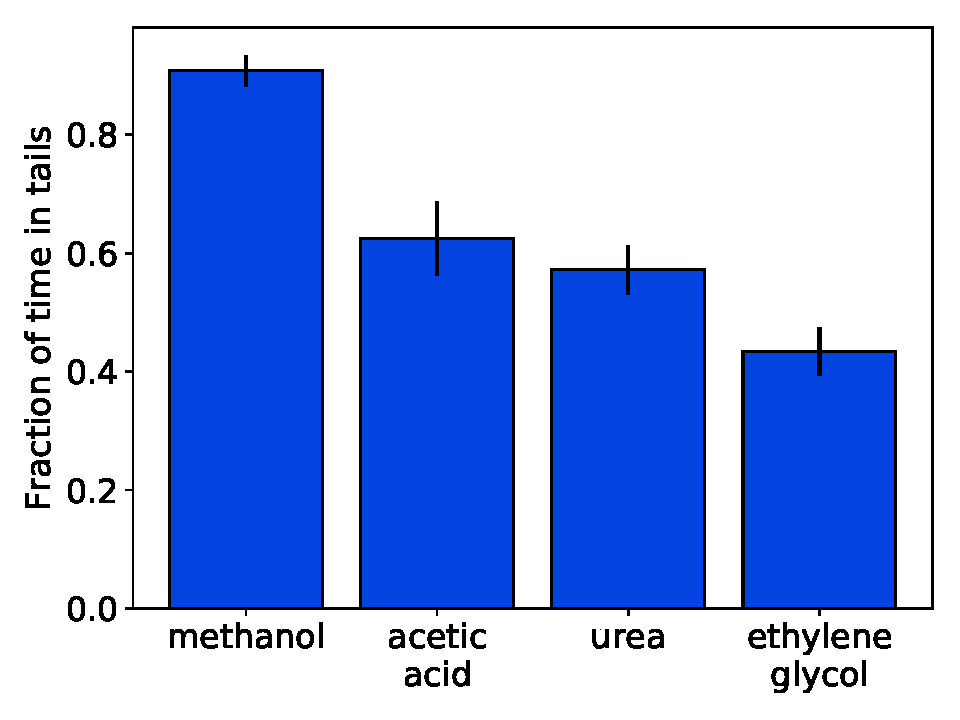
\includegraphics[width=0.5\textwidth]{AD_mode_occupation.pdf}
  \caption{Solutes spend various amounts of time in the tail and pore region dependent
  on their size, shape and chemical functionality. Methanol's small size favors 
  occupation of the much larger accessible volume in the tails. Urea and acetic acid
  are fairly stable in both regions since they are small and hydrophilic. Ethylene 
  glycol has a slight preference for the pores likely because it is a larger
  molecule with two hydrophilic hydroxyl groups.}\label{fig:AD_mode_occupation}
  \end{figure}
  
  Overall, the AD model does a reasonable job of predicting solute MSDs and its 
  parameters can help us further understand solute dynamics. Hops appear to be well
  modeled as anti-correlated draws from Gaussian and L\'evy stable distributions. 
  The data strongly suggests that one must truncate the power law dwell time 
  distributions in order to obtain accurate MSD estimates. We can further understand
  solute dynamics by adding radially dependent parameter distributions as in the 
  2 mode model. A significant amount of solute trajectory data is necessary 
  in order to achieve good parameter estimates. The exact amount of data required 
  is dependent on the solute studied. 
  
  %Solutes which achieve higher MSDs
  %in a given amount of time appear to be more accurately parameterized.
  
%  The parameters of the 1 mode model indicate some diversity in solute behavior. The value
%  of $\alpha_d$ for pure and truncated power law fits to the dwell time distributions of 
%  urea, ethylene glycol and methanol are similar. The value of $\alpha_d$ for acetic
%  acid is significantly lower than the rest of the solutes meaning it stays trapped 
%  for long periods of time more frequently. The value of $\lambda$ is largest for
%  methanol indicating that its longest dwell time is shorter than the longest dwell
%  times of all other solutes. When hops are fit to a Gaussian, it is clear that acetic
%  acid takes the smallest hops while methanol takes the largest. If we fit hops to a
%  L\'{e}vy stable distribution, we observe a similar trend in $\sigma$ values, but 
%  with varying weights on the distribution's tails. Acetic acid has the heaviest
%  tails (lowest $\alpha_h$), meaning it is more likely to take large hops, while 
%  ethylene glycol stays close to a Gaussian distribution (i.e. $\alpha_h$ near 2).
%  The Hurst parameters indicate a moderate degree of anti-correlation between hops. 
%  Surprisingly, methanol takes the most anti-correlated hops (lowest $H$). This is
%  likely because methanol spends the largest fraction of its time within the pores. 
%  It can still make large hops thanks to its small size, but tends to bounce around
%  the tails.

%  BJC4: urea and ethylene glycol only
%  The parameters of the 1 mode model are similar between urea and ethylene glycol which 
%  is not surprising considering their similar MD MSDs. Dwell times by 
%  ethylene glycol are shorter as shown by its larger $\alpha_d$ and $\lambda$ values. Both
%  solutes make similarly sized hops with hop distributions that are relatively close 
%  to Gaussian (i.e. $\alpha_h$ near 2) when fit to a L\'evy stable distribution. Finally,
%  both solutes exhibit a similar degree of correlation between hops with ethylene glycol
%  exhibiting motion closer to Brownian. 
  
%  The difference in parameters of each mode of the 2 mode sFBM model offer additional
%  mechanistic insight which the 1 mode model lacks. It is clear that solutes are 
%  significantly slowed while they are in the tail region (mode 2) where long dwell times
%  are more probable and hops are smaller (smaller $\alpha_d$). 
% BJC: I'm not sure how valid it is to analyze lambda because it is dependent on alpha. There is some counterbalancing going on.  
% The values of $\lambda$, however, do not 
% appear to be directly correlated to mode. For example, $\lambda$ for ethylene glycol is
% lower in the pores, meaning its longest dwell times in the pores are longer than its
% longest dwell times in the tails. This may be a consequence of    
%  Interestingly, $\alpha_h$ for urea and acetic acid in mode 2 is 1.50 meaning its 
%  hop distribution is heavy tailed relative to ethylene glycol and methanol whose 
%  $\alpha_h$ values are more consistent with a Gaussian distribution. Acetic acid and
%  urea are structurally similar molecules, both planar with two heavy atoms attached to
%  a carbonyl group. Their small size and rigid shape may allow them to slip through 
%  gaps in the tails. Meanwhile, methanol is small enough that it does not need to make 
%  larger jumps to escape traps. 
  
%  BJC4: Urea and ethlyene glycol only
%  The parameters of the 2 mode model are again similar between urea and ethylene glycol, 
%  but the difference between parameters of each mode offer more detailed mechanistic
%  insight than the 1 mode model. It is clear that solutes are significantly slowed while
%  they are in the tail region where long dwell times are more probable (lower $\alpha_d$)
%  and hops are smaller (smaller $\sigma$).  
%  Interestingly, $\alpha_h$ for urea in mode 2 is 1.50 meaning its hop distribution is
%  heavy tailed relative to ethylene glycol which has an $\alpha_d$ more consistent 
%  with a Gaussian distribution. Although urea's $\sigma$ parameter is much smaller in 
%  the tails, it still has an appreciable probability of making large hops. This could 
%  be a consequence of urea's relatively small size and rigid shape compared to ethylene glycol.
  %Ethylene glycol is a linear chain that can
  %easily become entangled among the alkane tails while urea is planar with its four
  %heavy atoms bonded to a single central atom.
 
  
  %BJC3: Is it a bad idea to acknowledge that there is no experimental data? I can 
  % spin this paragraph in a different way.
  %MRS4: can one to training and validation?  Train on 1/2 the data, then see how well it fits the other half?
  %MRS4: also, you need to be more specific about choosing for WHAT purpose.  Different purposes could imply different models.
%  Choosing which model to use for long timescale projections is not entirely obvious
%  without experimental data to compare with. For our comparisons to MD, using a 
%  truncated power law distribution is an obvious choice. However, given that extremely
%  long dwells are a rare event, it is possible that studying a much larger set of 
%  solutes will fill in the tail of the pure power law PDF. Regarding hop length 
%  distributions, the generality of L\'evy stable distributions is powerful, but the
%  lack of exact methods for simulation of fractional L\'evy motion reduces it's 
%  accuracy and computational tractability. Treating the dynamics as fractional 
%  Brownian motion is probably sufficient unless the L\'evy index, $\alpha_h$, is well below 2.
  
%  \noindent We can use the model to project our simulations out to very long timescales.
%  \begin{itemize}
%    \item We can not definitively say which combination of distributions are best to use.
%    \item Although the longest observed dwell times and hop lengths are less than
%    the length of the simulated trajectories and box lengths respectively, it is still possible
%    that that extremely long dwell times and hops are observed experimentally in rare but
%    significant cases.
%    \item We present long timescale projections using combinations of each distribution in the
%    table below
%  \end{itemize}

  % BJC2: table of long timescale projections using combinations of dwell and hop distributions. 
  %% TABLE %%

  \subsection{The Markov State-Dependent Dynamical Model}\label{section:msm_results}
  
  %BJC4: added transitional paragraph
  The AD model is useful if one does not know exact transport mechanisms 
  in a system since it only requires time series data. However, since we have
  already studied transport mechanisms in detail in our previous work, we can
  attempt to model transport as transitions between known discrete
  states, defined in Table~\ref{table:states}, with state-dependent positional
  fluctuations, which we 
  %MRS6:
  refer to as
  %call 
  the MSDDM.
  %MRS6: maybe give full name before if you are essentially defining it. 

  % BJC4: I moved this discussion up. It used to be after I presented the parameters
  Solute size and chemical functionality influence which states are visited most frequently.
  In Figure~\ref{fig:state_probabilities}, we plotted the probabilities of occupying
  a given state at any time. Solutes tend to favor the same types of interactions 
  independent of which region they are in.

  % BJC5: moved to previous section  
%   Urea and acetic acid spend slightly more than half of
%  their time in the tails (56\% and 62\% of their time respectively) while ethylene
%  glycol spends about 44\% of its time in the tails. Urea and acetic acid's compact
%  and flat structure allows it to more easily partition into the tails while ethylene
%  glycol prefers the pore region due to its two hydrophilic hydroxyl groups. Meanwhile
%  methanol spends 91 \% of its time in the tails likely due to its small size.
  
  \begin{figure}
  \centering
  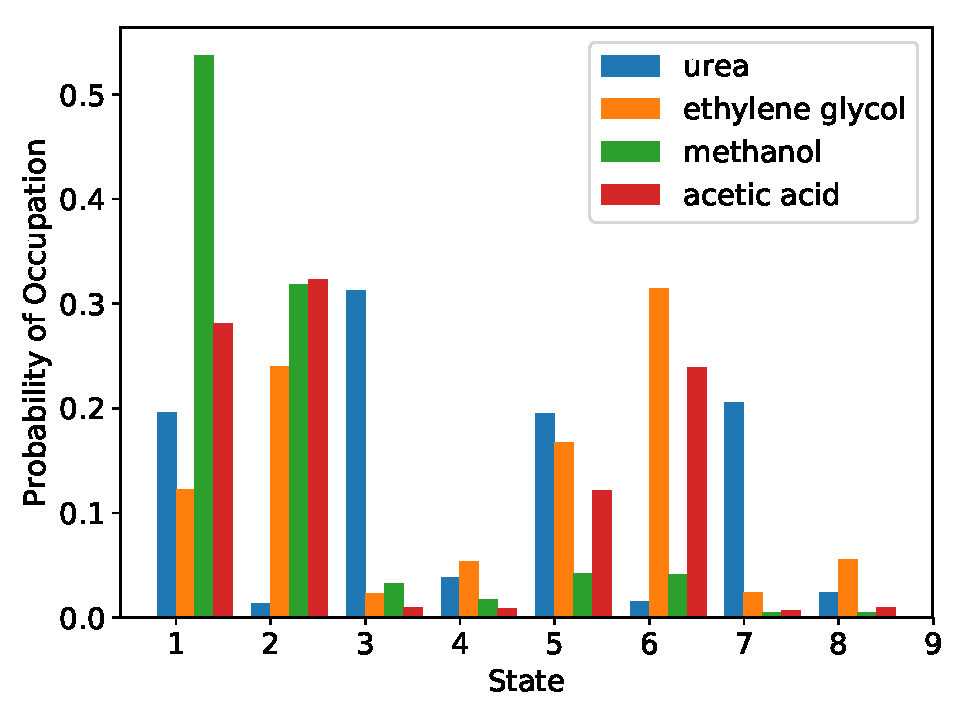
\includegraphics[width=0.475\textwidth]{state_probabilities.pdf}
  \caption{Solutes spend varying amounts of time under the influence of each
  trapping mechanism. To aid the reader, we labeled each state with an abbreviation which
  identifies the combination of conditions to which each solute is subject in each state:
  t - tails, p - pores, h - hydrogen bonded, a - associated with sodium. Solutes tend to 
  favor the same types of interactions (e.g. hydrogen bonding and/or associating with sodium
  ions) independent of whether they are in the pores or the tails.}\label{fig:state_probabilities}
  \end{figure}
  
  Urea spends the largest fraction of its time trapped via association with sodium ions.
  It does so 31\% of the total time while in the tails (state 3) and 21\% of the
  total time while in the pores (state 7). Note that sodium does not drift significantly 
  into the tails but sits close to the pore/tail region boundary. The electron-dense 
  and unshielded oxygen atom of urea's carbonyl group is prone to associate with 
  positively charged sodium ions. The nitrogen atoms of urea are only weak hydrogen bond
  donors.
  
  Ethylene glycol spends the largest fraction of its time trapped in a hydrogen
  bonded state. It does so 24\% of the total time while in the tails (state 2)
  and 32\% of the total time while in the pores (state 6). The two hydroxyl groups 
  of ethylene glycol readily donate their hydrogen atoms to the carboxylate
  head groups and the ether linkages between the head groups and monomer tails. 
  
  Methanol spends most of its time unbound in the tail region (state 1) and spends a 
  significant portion of time hydrogen bonded while in the tail regions.
  Tail region hydrogen bonds are donated from methanol to the ether linkages between
  the monomer head groups and tails.
  
  Finally, acetic acid spends the majority of its time hydrogen bonding both in and out
  of the pore (states 2 and 6). Although it has an unshielded carbonyl group in its
  structure, association with sodium ions in this environment is apparently a much 
  weaker interaction than hydrogen bonding.
  
  To create an MSDDM for each solute, we determined the state sequence associated
  with each solute trajectory and then generated emission distributions of fluctuations
  within each state as well as transitions between states. There are not enough 
  consecutive observations of each type of transition with which to study their 
  individual correlation structures so we grouped all transition distributions
  into a single distribution and measured the correlation of the series of all 
  transitions. 
  %MRS6: how much of this is described earlier in methods?
  We lose information about individual types of transitions, however, 
  we believe this is unavoidable without at least an order of magnitude of additional data.
  In theory, one could parameterize separate transition distributions for those
  which occur in the tails versus in the pores, however this would lead to a broken 
  correlation structure similar to that seen in the 2 mode AD model.

  We observe correlated emissions drawn from L\'evy stable distributions. The 
  deviation of the emission distributions from Gaussian behavior is far more pronounced
  than that seen in the hop length distributions of the previous section, therefore we 
  did not consider the Gaussian case (see Figure~\ref{fig:gaussian_levy_comparison}).
  The correlation structure between hops resembles that of FLM (Figure~\ref{fig:msddm_acf}).
  The parameters of the L\'evy stable distributions along with their Hurst parameters 
  are visualized in Figure~\ref{fig:msddm_parameters} (and tabulated in the Supporting
  Information, Table~\ref{S-table:msddm_params}). 
  
  \begin{figure}
  \centering
  \begin{subfigure}{0.49\textwidth}
  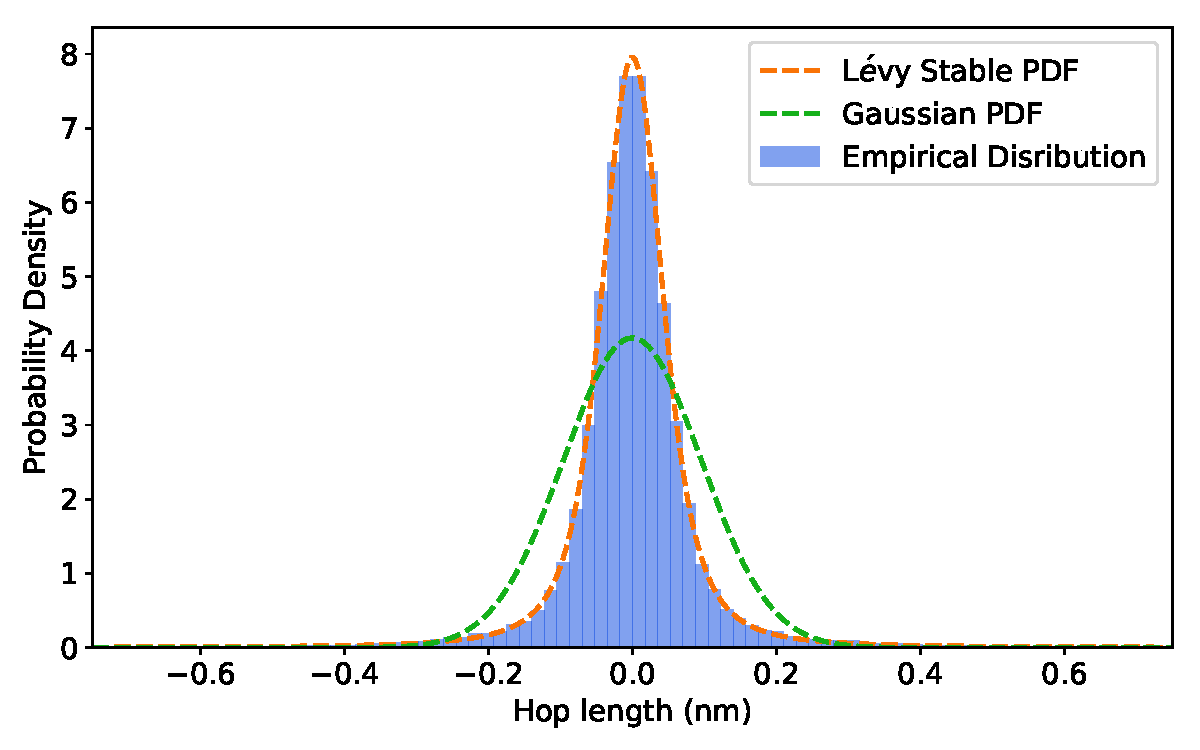
\includegraphics[width=\textwidth]{gaussian_levy_comparison.pdf}
  \caption{}\label{fig:gaussian_levy_comparison}
  \end{subfigure}
  % /figures/msddm_acf.py
  \begin{subfigure}{0.42\textwidth}
  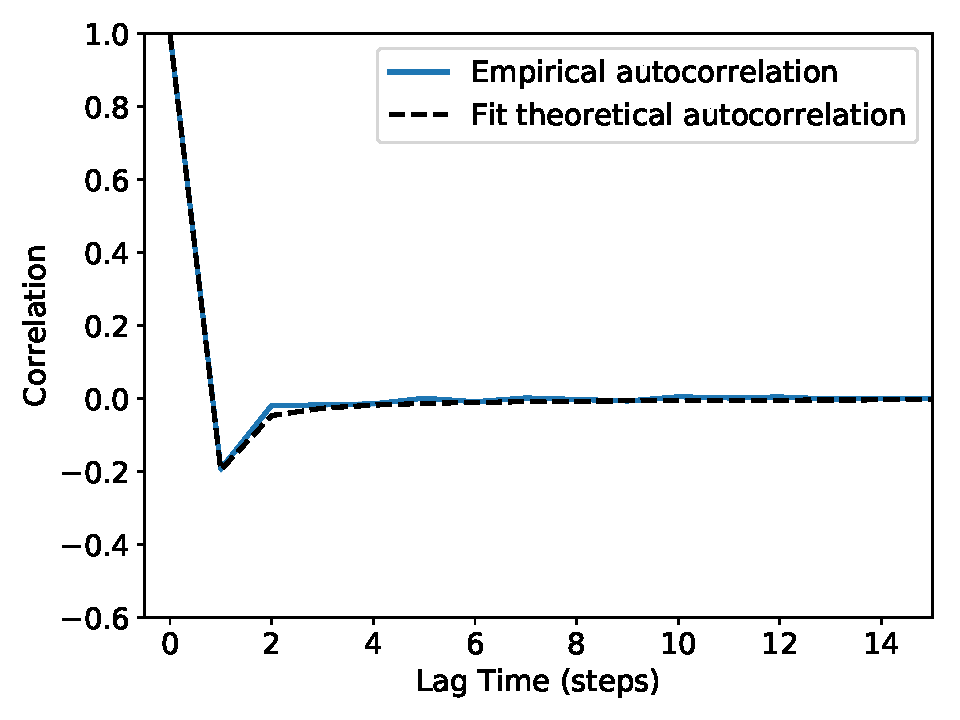
\includegraphics[width=\textwidth]{msddm_acf.pdf}
  \caption{}\label{fig:msddm_acf}
  \end{subfigure}
  \caption{(a) Emission distributions are non-Gaussian and heavy-tailed. Shown here is the
  emission distribution for transitions between states. The maximum likelihood
  Gaussian fit severely underestimates the empirical density of hops near and far from zero 
  while overestimating the density of hops at intermediate values. (b) Jumps drawn from
  the transition distribution are negatively correlated to each other. The normalized version 
  of Equation~\ref{eqn:flm_autocovariance} fits well to the data suggesting FLM is
  an appropriate way to model jumps.} \label{fig:msddm_emissions}
  \end{figure}
  
  \begin{figure}
  \centering
  \begin{subfigure}{0.325\textwidth}
  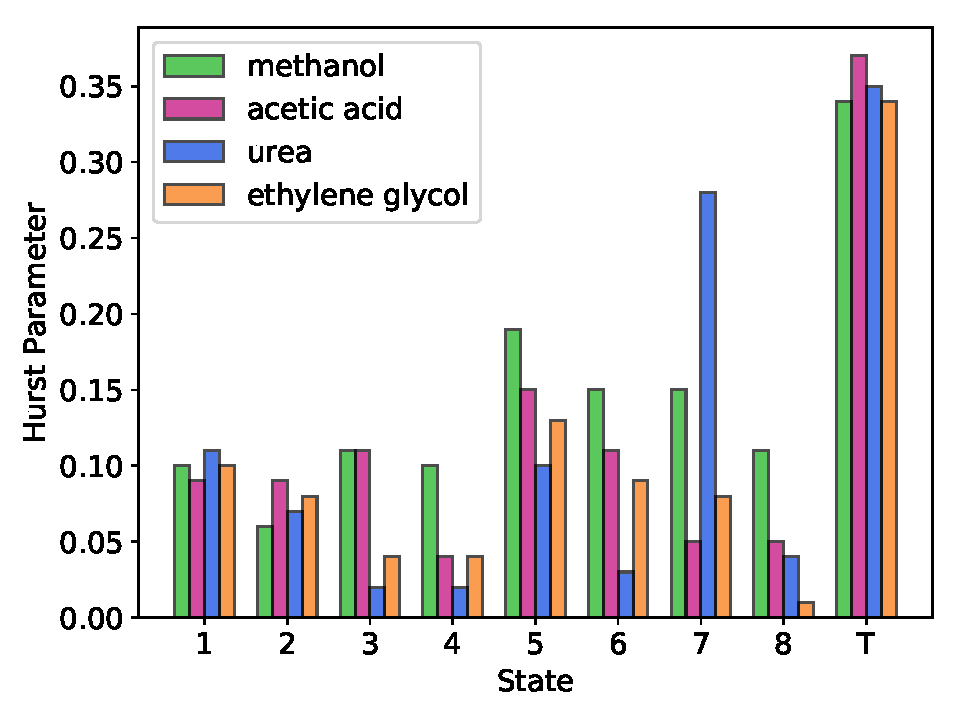
\includegraphics[width=\textwidth]{H_v_state.pdf}
  \caption{}\label{fig:H_v_state}
  \end{subfigure}
  \begin{subfigure}{0.325\textwidth}
  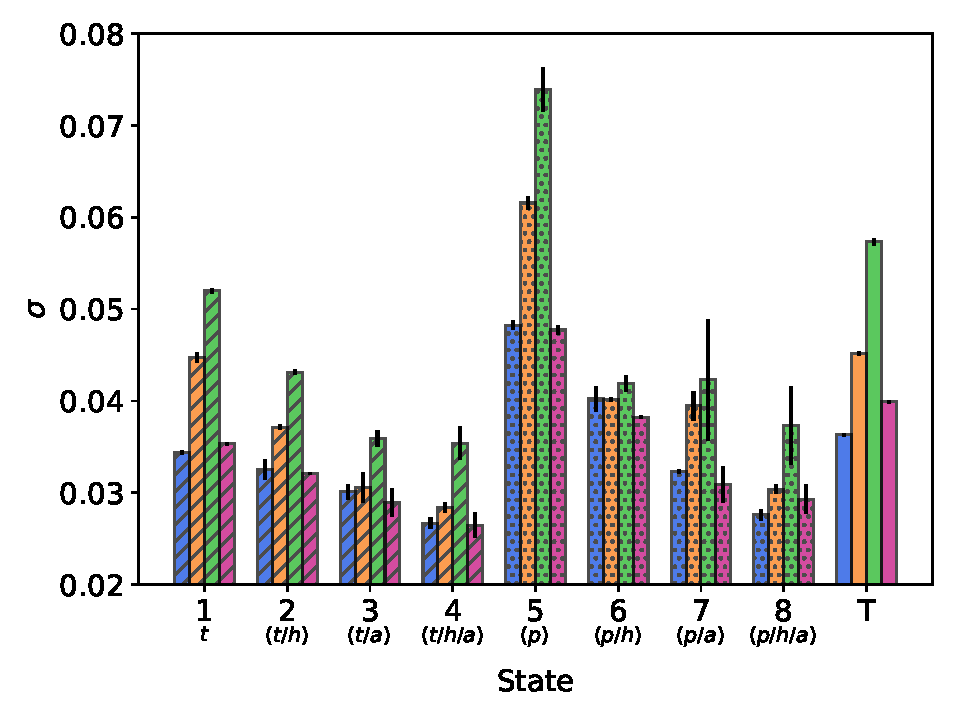
\includegraphics[width=\textwidth]{sigma_v_state.pdf}
  \caption{}\label{fig:sigma_v_state}
  \end{subfigure}
  \begin{subfigure}{0.325\textwidth}
  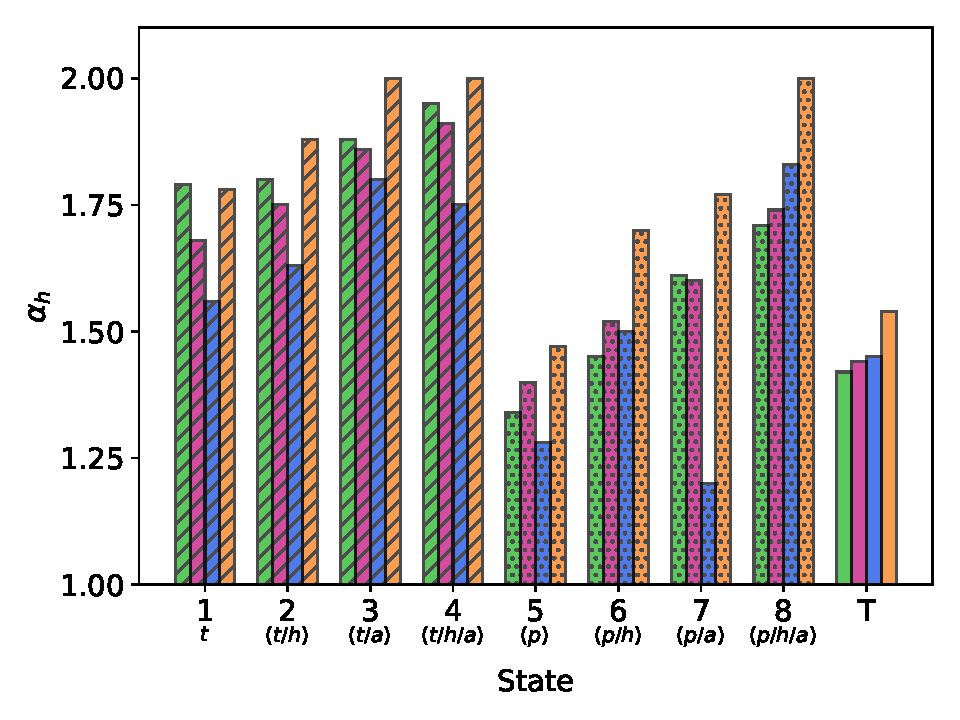
\includegraphics[width=\textwidth]{alpha_v_state.pdf}
  \caption{}\label{fig:alpha_v_state}
  \end{subfigure}
  \caption{The parameters of the MSDDM are strong functions of trapping mechanisms.
  We observe different parameters but with similar trends between the tail and pore
  region. The states are defined in Table~\ref{table:states}. See Figure~\ref{fig:state_probabilities}
  for a description of the abbreviation under each state number. The legend in (a) applies to all subplots. (a) Motion is
  highly anti-correlated in trapped states. As the number of simultaneously influencing
  trapping mechanisms increases, the Hurst parameter decreases. The Hurst parameter is
  highest during transitions between states (state T). (b) As more trapping mechanisms
  simultaneously influence solutes, the width of the hop length distribution decreases.
  The largest hops occur when solutes are unbound in the pores. (c) The weight of the 
  hop length distribution's tails, parameterized by $\alpha_h$, increases as more trapping
  mechanisms influence solutes simultaneously. The transition hop distributions have
  among the heaviest tails.}\label{fig:msddm_parameters}
  \end{figure}

  Most of a solute's MSD is a consequence of transitions between the 8 states
  in Table~\ref{table:states}. Motion while trapped in a state is highly 
  anti-correlated as indicated by their consistently low Hurst parameters.
  Perfectly anti-correlated motion ($H$=0) results in no contribution to the solute's
  MSD. There is a weak negative trend in the Hurst parameter values as the number
  of simultaneously influencing trapping mechanisms increases (Figure~\ref{fig:H_v_state}). 
  Surprisingly, state 5 $H$ values are low despite the solutes being subject to no
  trapping mechanisms. Highly anti-correlated behavior in the pores in the absence of
  any trapping mechanism is likely caused by collisions with monomer head groups 
  within the pore region. The Hurst parameters for transitional (T) emissions are up to 
  18 times higher than emissions from trapped states. The value of $\alpha_h$ for 
  transition emissions is also relatively low giving higher probabilities to larger hops.
  
  As solutes are influenced by more trapping interactions simultaneously (e.g.~hydrogen
  bonding \textit{and} association with sodium versus just hydrogen bonding), the 
  width of the hop length distribution, $\sigma$, decreases while its L\'evy index,
  $\alpha_h$, increases. Treating states in the tail and pore regions independently, 
  $\sigma$ is largest and $\alpha_h$ is smallest when solutes are not hydrogen bonding
  or associating with sodium (states 1 and 5). Solutes are free to move and take 
  occasionally large hops. The smallest $\sigma$ and highest $\alpha_h$ values are
  measured when solutes are hydrogen bonding and associating with sodium at the
  same time (states 4 and 8). Motion is restricted by multiple tethers which 
  maintains a relatively narrow distribution of hop lengths.
  
%  The trapping mechanisms affect each solute to varying degrees. The probabilities
%  of occupying a given state at any time are plotted in Figure~\ref{fig:state_probabilities}.
%  Urea and acetic acid spend slightly more than half their time in the tails (56\% and 62\% 
%  of their time respectively) while ethylene glycol spends about 44\% of its time in the tails.
%  Urea and acetic acid's compact and flat structure allows it to more easily 
%  partition into the tails while ethylene glycol prefers the pore region due to 
%  its two hydrophilic hydroxyl groups. Meanwhile methanol spends 91 \% of its 
%  time in the tails likely due to its small size.

%MRS6: even if the MSD is well predicted, if the trajectories look different, can it really be a useful model?  I.e. is one getting the right answer for the wrong reasons?  What does it mean if MSD's are good, but the dwell times are not great?
  Qualitatively, realizations of the MSDDM are not consistent with MD solute
  trajectories. Using the parameters shown in Figure~\ref{fig:msddm_parameters}
  we generated realizations of the MSDDM and plotted a typical realization for each
  solute in Figure~\ref{fig:msddm_eyetest}. Except in rare cases, the solutes do not make
  large hops. There are two reasons for this behavior. First, the width of 
  hop length distributions are much smaller than those of the AD model. Closer
  examination of urea's MD trajectories shown in Figure~\ref{fig:solute_trajectories} 
  reveal that hops tend to be an accumulation of a series of hops in the same direction.
  All of the hops in the MSDDM are negatively correlated which prevents this from happening.
  The second reason is a consequence of using a single hop length distribution 
  for transitions. Many transitions occur between two trapped states where the 
  transitional hops are actually very small. Our model ignores this physical 
  restriction which can cause the solute to drift rather than stay trapped.
  
  \begin{figure}
  \centering
  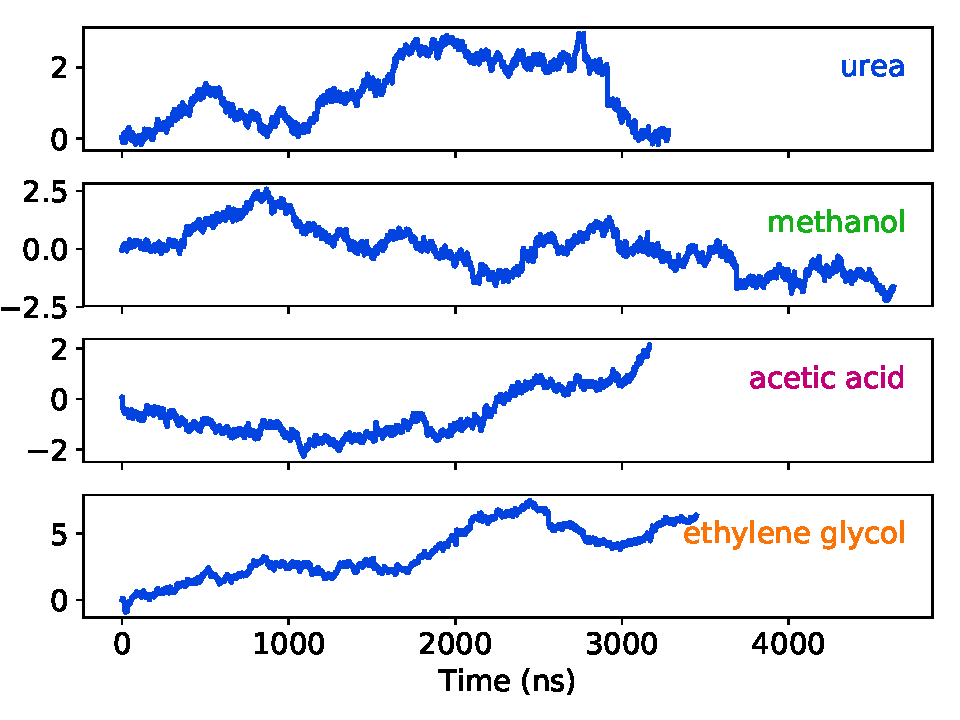
\includegraphics[width=0.5\textwidth]{msddm_realizations.pdf}
  %MRS6: see above - right for wrong reasons?
  \caption{Realizations of the MSDDM for each solute do not reproduce the hopping
  and trapping behavior observed in our MD simulations. Except for a few large 
  hops, the trajectories are qualitatively similar to what one might expect for
  Brownian motion. Note that the length of the realizations are equal to the length
  of the equlibrated portion of the MD trajectories for each solute.}\label{fig:msddm_eyetest}
  \end{figure}
  
  %Methanol's
  %MSD is over-predicted at short timescales while acetic acid's entire MSD 
  %curve is severely over-predicted.
  
  \begin{figure}
  \centering
  \begin{subfigure}{0.45\textwidth}
  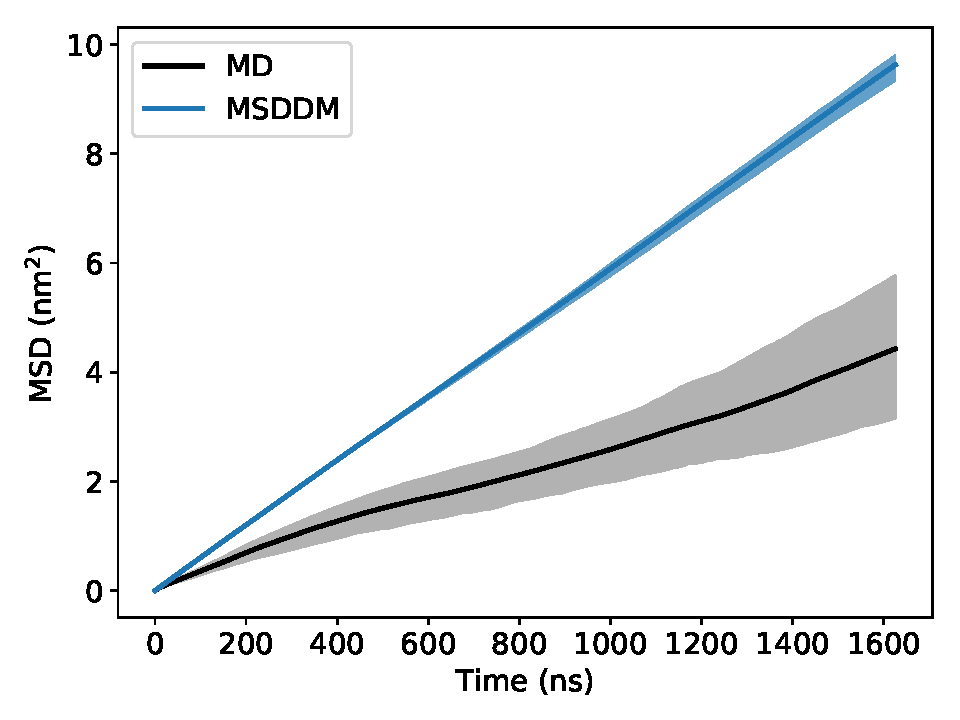
\includegraphics[width=\textwidth]{URE_msddm.pdf}
  \caption{Urea}\label{fig:URE_msddm}
  \end{subfigure}
  \begin{subfigure}{0.45\textwidth}
  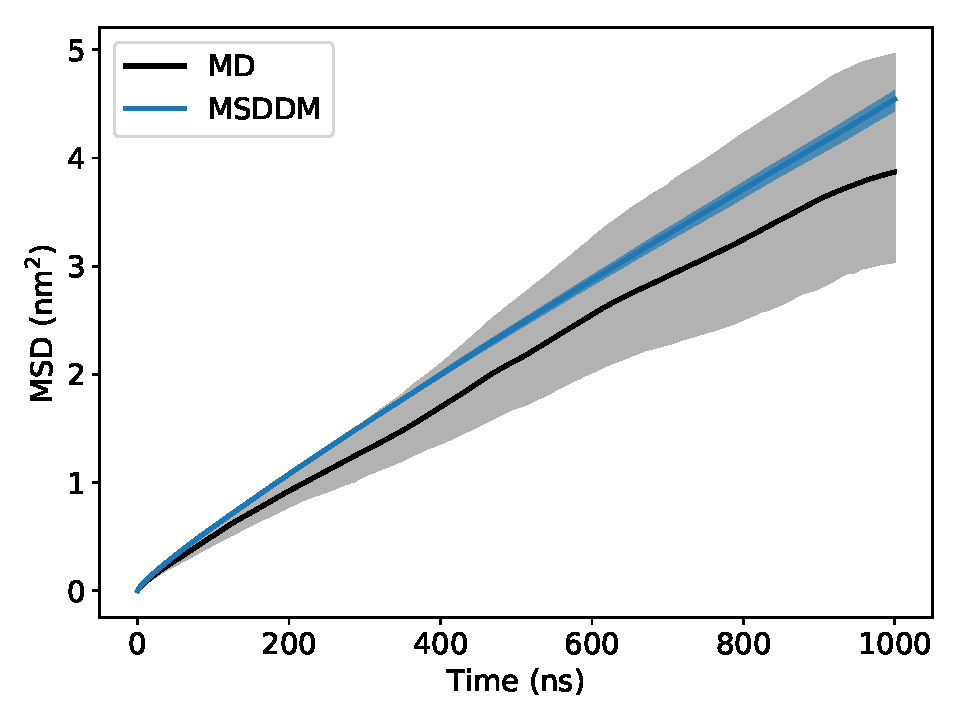
\includegraphics[width=\textwidth]{GCL_msddm.pdf}
  \caption{Ethylene Glycol}\label{fig:GCL_msddm}
  \end{subfigure}
  \begin{subfigure}{0.45\textwidth}
  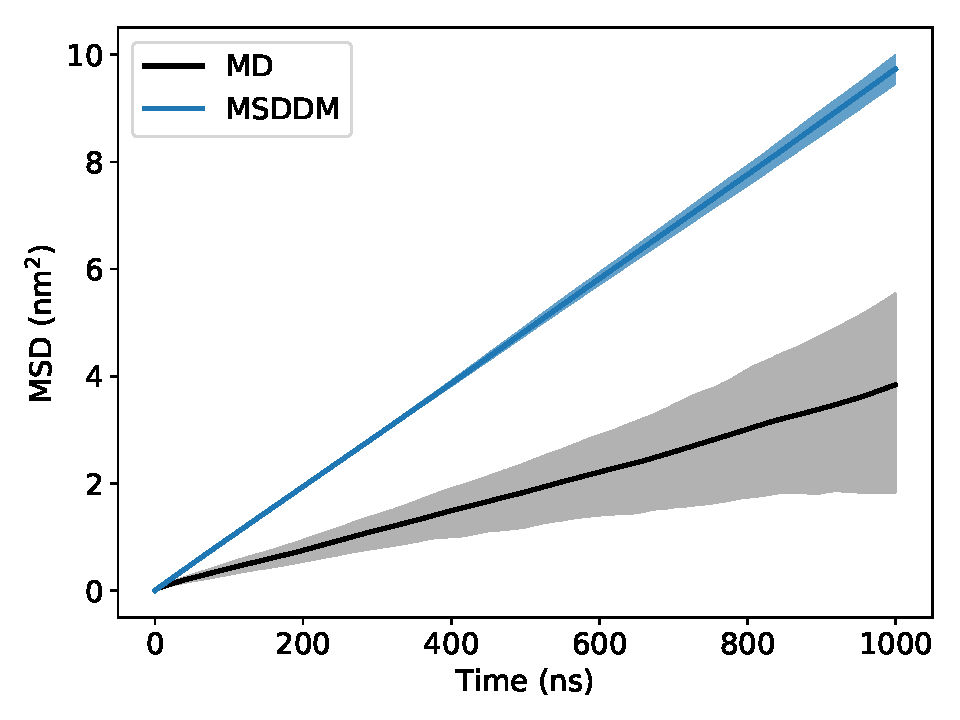
\includegraphics[width=\textwidth]{MET_msddm.pdf}
  \caption{Methanol}\label{fig:MET_msddm}
  \end{subfigure}
  \begin{subfigure}{0.45\textwidth}
  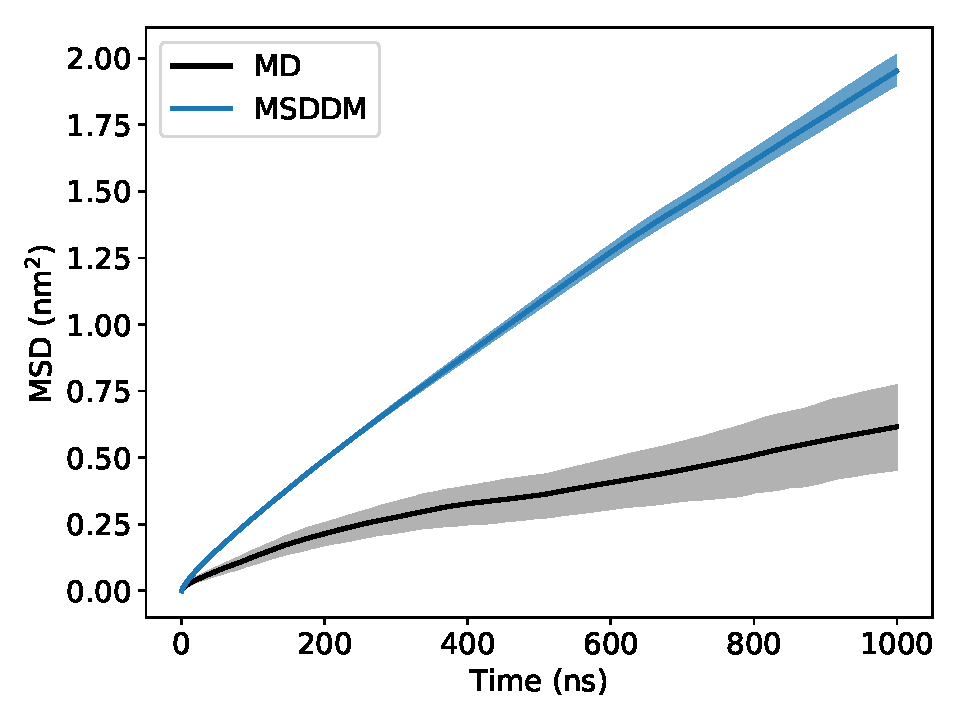
\includegraphics[width=\textwidth]{ACH_msddm.pdf}
  \caption{Acetic Acid}\label{fig:ACH_msddm}
  \end{subfigure}
  \caption{In most cases, the magnitude of the MSD curves predicted by the 
  MSDDM agree well with those generated from MD simulations. The predicted MSD
  curves of urea and ethylene glycol lie within the 1$\sigma$ confidence 
  intervals of MD for all time lags. Methanol over-predicts the MSD at small
  time lags and acetic acid grossly over-predicts the MSD at all time lags.
  Like the anomalous diffusion model, the MSDDM doesn't fully capture the 
  curvature of the MD MSD curves. }\label{fig:msddm_performance}
  \end{figure}
  
  Despite qualitative differences in trajectory realizations, the dynamics of 
  urea, ethylene glycol and, to a lesser extent, methanol appear to be well-captured
  by the MSDDM. We simulated 1000 MSDDM trajectory realizations for each solute, as
  described in Section~\ref{method:MSMs}, then calculated their MSDs (see 
  Figure~\ref{fig:msddm_performance}). In most cases, the MSDDM predicts the magnitude of the MD MSDs 
  within their 1$\sigma$ confidence intervals. One could argue that the curves
  of ethylene glycol and urea are statistically indistinguishable. However, 
  it's possible that they may diverge on longer timescales due to differences
  in their curvature. Similarly, methanol's MD MSD is nearly linear while 
  the MSDDM prediction is curving downward implying that it may underestimate
  the MSD on longer timescales. 
  
  The predicted MSD of acetic acid is severely over-estimated most likely due
  to poor parameterization. 
  %MRS6: poor parameterization is vague.  Of which features?
As stated earlier, most of a solute's motion is 
  due to displacements during state transitions. Acetic acid has a transitional
  Hurst parameter close to urea's and a transitional $\sigma$ value that 
  is higher than urea's. This suggests that the heavier tails of urea's transitional
  hop distribution (greater $\alpha_h$ value) are in large part responsible for 
  urea's higher predicted MSD. Although, note that acetic acid's predicted MSD
  actually lies just within the lower bound of Urea's MD MSD 1$\sigma$ 
  confidence interval. There is also the strong possibility that the over-estimate is
  a consequence of lumping together all of acetic acid's transitional hops into
  a single correlated distribution.
  
  The MSDDM suffers similar shortcomings to the AD model. First, curvature 
  on long timescales due to positional anti-correlation may result in 
  underestimates of the MSD at large time lags. As suggested earlier, truncating
  the positional autocorrelation function may help solve this issue. Second, 
  parameterization can be challenging. In addition to possibly poor estimates 
  of the Hurst parameter, we made the simplifying assumption that we could lump
  all transitional hops into a single distribution. While this appears to work
  in most cases, it is the source of qualitative mismatches between MSDDM
  realizations and MD simulation trajectories and it may be the source of the 
  over-estimate of acetic acid's MSD.
  
  The MSDDM offers mechanistic insight and, in 3 out of 4 cases, gives reasonable
  predictions of solute MSDs. To successfully apply the model, one must know 
  representative discrete states beforehand or apply some technique to identify
  them. At the very least, we can used the MSDDM to obtain a detailed quantitative
  picture of dynamics within each state in terms of the magnitude of their 
  fluctuations and correlation with previous motion. If we have confidence in
  their predictive ability, then we can project solute trajectories out to 
  macroscopic timescales and estimate macroscopic observables such as solute 
  flux and selectivity.
  
%  Unfortunately correlation between adjacent same-state sequences is lost
%  with our model which causes the MSDs to be significantly over-predicted. The MSDDM
%  may be suitable for processes with rarer transitions between states. If we can 
%  further reduce the state-space of our models, it may have better predictive success,
%  but we lose mechanistic detail.
  
% BJC5: following not true
%  The MSDDM overestimates solute MSDs because correlation is lost every time a
%  state switch occurs. Although correlation exists within each sequence, there
%  is no memory of the previous state or state transition that can be built into
%  the first emission of the most recent state. This implies that the first 
%  value in a state sequence is a random draw from the underlying emission 
%  distribution. Frequent transitions between states lead to an abundance of 
%  short dwell times. It is difficult to accurately correlate short sequences so
%  we are almost simulating uncorrelated draws from the emission distribution.
%  In Figure~\ref{fig:T_sensitivity}, we demonstrate this effect by varying the
%  transition matrix and simulating a simple 2-state model with parameters similar
%  to those in Table~\ref{table:msddm_params} (we tabulated the parameters used 
%  in Table~\ref{S-table:msddm_params} of the Supporting Information). We modified
%  the probability transition matrix, $T$, in order to control the probability of 
%  self-transitions (the diagonal elements of $T$). Larger self-transition 
%  probabilities lead to longer dwell times in each state. We set the off-diagonal
%  elements of $T$ to be equal values that make the rows of $T$ sum to unity when
%  combined with the self-transition probabilities. As we increase the 
%  self-transition probability, $T_{ii}$, the simulated MSD decreases. Consequently,
%  longer dwell times in each state allow us to more accurately simulate the
%  negative correlation that we observe in MD.
%  
%  \begin{figure}
%  \centering
%  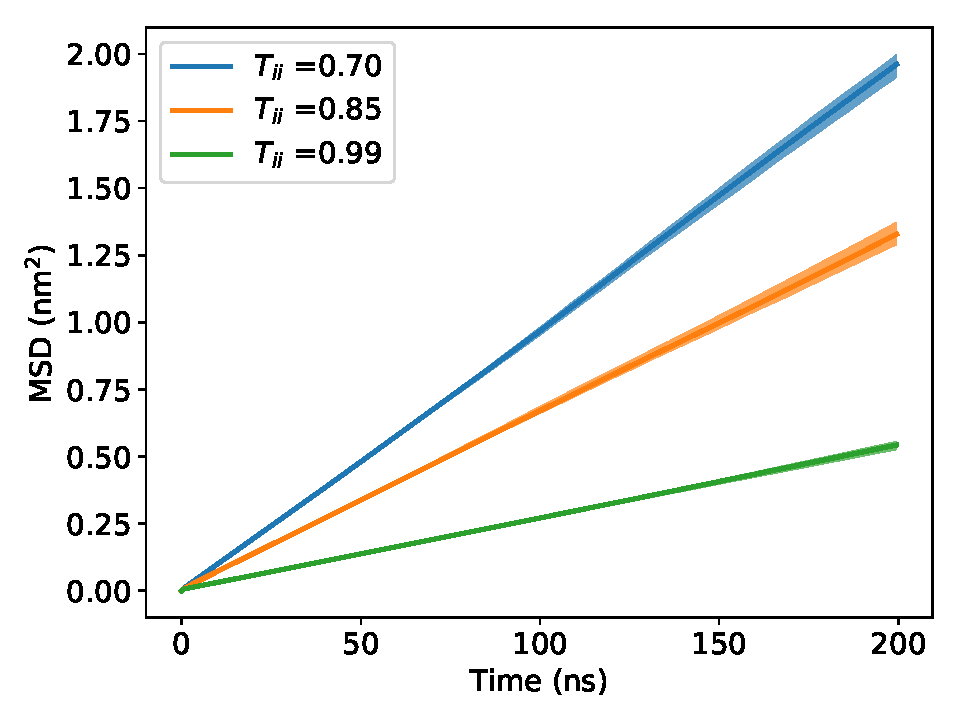
\includegraphics[width=0.5\textwidth]{T_sensitivity.pdf}
%  \caption{As we increase the self-transition probabilities ($T_{ii}$) of an MSDDM,
%  the simulated MSD of the process decreases because the negative correlation structure
%  of individual state sequences is simulated more accurately.}\label{fig:T_sensitivity}
%  \end{figure}
  
  \subsection{Solute Flux}\label{section:mfpt}
  
  %MRS6: to what extent can be 'cut' models be the ones used, and the untruncated ones thrown out early in the paper to simplify the presentation. 
  We used the 1-mode sFBMcut (see Table~\ref{table:anomalous_models}) anomalous 
  diffusion model and the MSDDM in order to demonstrate how one can use their realizations
  in order to calculate the flux (see section~\ref{method:mfpt}) of solutes given model 
  parameters extracted from MD simulations. The 1-mode sFBMcut model generates predictions
  similar to the 1-mode sFLMcut model at a lower computational cost and is far more
  accurate than sFBM and sFLM. We showed that the 2-mode AD model has a broken correlation
  structure, so we do not consider it here.

  %BJC4: not sure if the next couple paragraphs belong in methods 
  %MRS5: this could potentially be in methods.  Alternatives can be discussed there.
  %BJC5: I tried putting this in methods, but it feels weird without stating the
  % empirical equation. And I'm avoiding stating the empirical model in the methods
  % since it is informed by the data.
  It is computationally infeasible to simulate trajectories long enough that they
  traverse the length of a macroscopic pore. To date, the thinnest H\textsubscript{II}
  LLC membrane synthesized with the monomer in this work was 7$\mu$m thick. Using
  24 cores to simulate trajectory realizations in parallel, it takes on the order 
  of 1 day to simulate 10000 sFBMcut realizations of solutes traversing a 50 nm pore.
  The computational requirements of the MSDDM are about 10 times longer. For both
  models, the RAM requirements and performance scales greater than linearly and 
  thus would take an infeasible amount of memory and time to simulate transport 
  through a pore over 100 times longer.
  
  We used simulated trajectories which traverse computationally-reasonable length
  pores in order to construct an empirical model which one can use to estimate 
  particle flux for arbitrary length pores. We fit Equation~\ref{eqn:passage_times}
  to the empirical distribution of first passage times in Figure~\ref{fig:fpt_distributions}
  and used the expected value of the analytical equation to calculate flux from 
  Equation~\ref{eqn:hill_relation}. As shown in Figures~\ref{fig:flux_curves_ad} and
  \ref{fig:flux_curves_msddm}, the flux appears to scale according to a power law 
  of the form:
  \begin{equation}
  J(L) = cL^{-\beta} 
  \label{eqn:flux_decay}
  \end{equation}
  %while the MFPT scales as its inverse, $(1/c)L^{\beta}$. 
  
  %BJC: need simulations with increased length for L=35-50 nm pores of acetic acid and methanol
  %BJC: see of clauset has better way of fitting t^-alpha (alpha might be too big)
  %BJC: should have a paragraph about c -- roughly follows their MSDs.
  \begin{figure}
  \centering
  %BJC5: TODO: make same figure for msddm
  \begin{subfigure}{0.325\textwidth}
  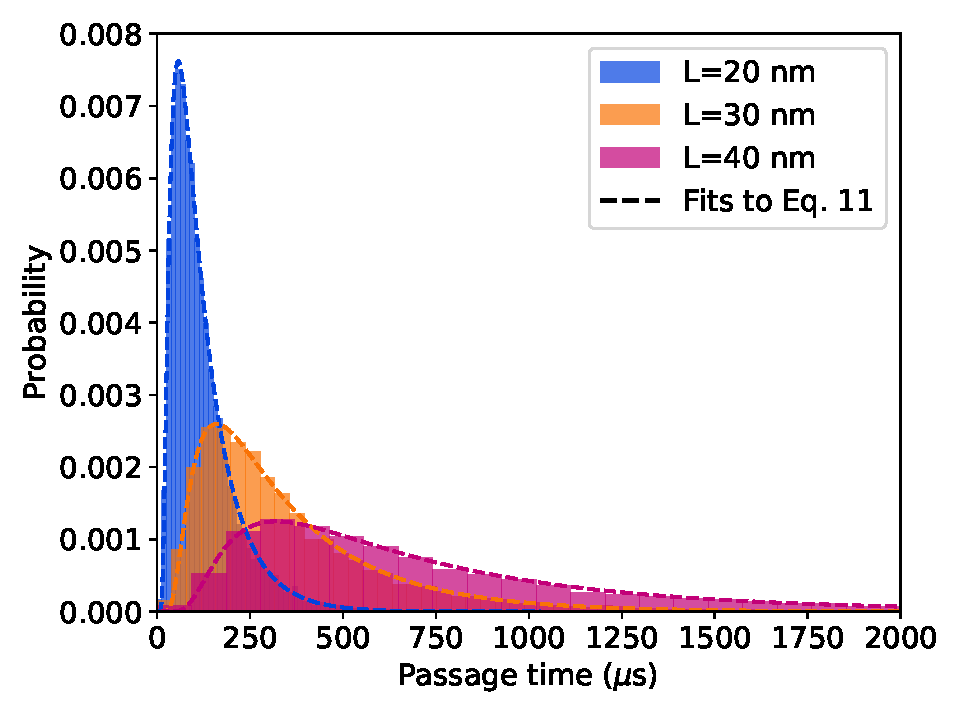
\includegraphics[width=\textwidth]{fpt_distributions.pdf}
  \caption{}\label{fig:fpt_distributions}
  \end{subfigure}
  \begin{subfigure}{0.325\textwidth}
  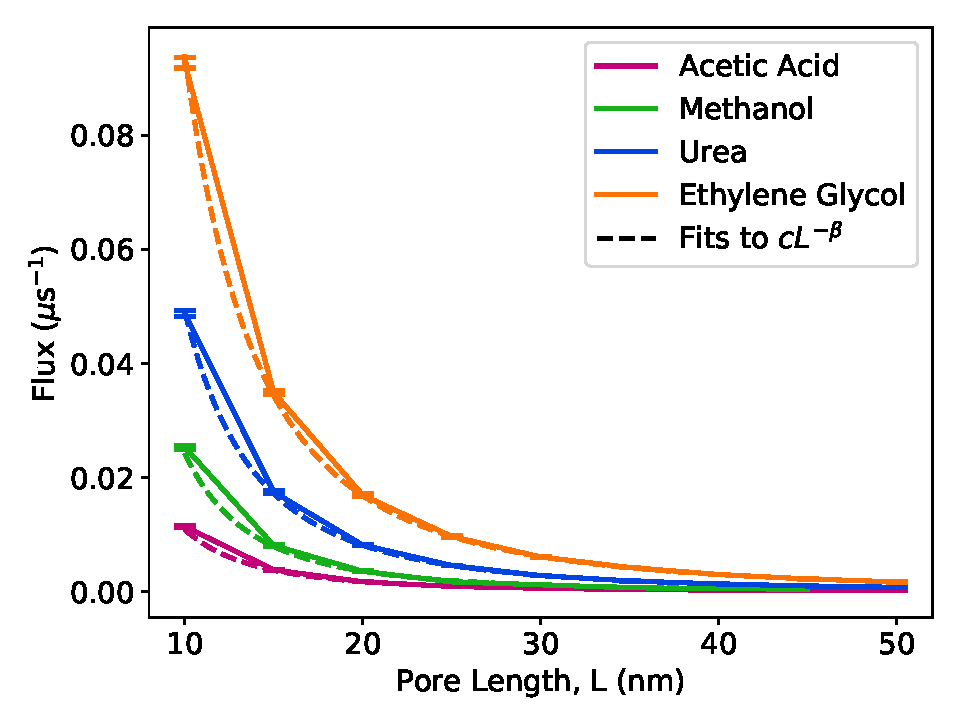
\includegraphics[width=\textwidth]{flux_curves.pdf}
  \caption{sFBMcut}\label{fig:flux_curves_ad}
  \end{subfigure}
  \begin{subfigure}{0.325\textwidth}
  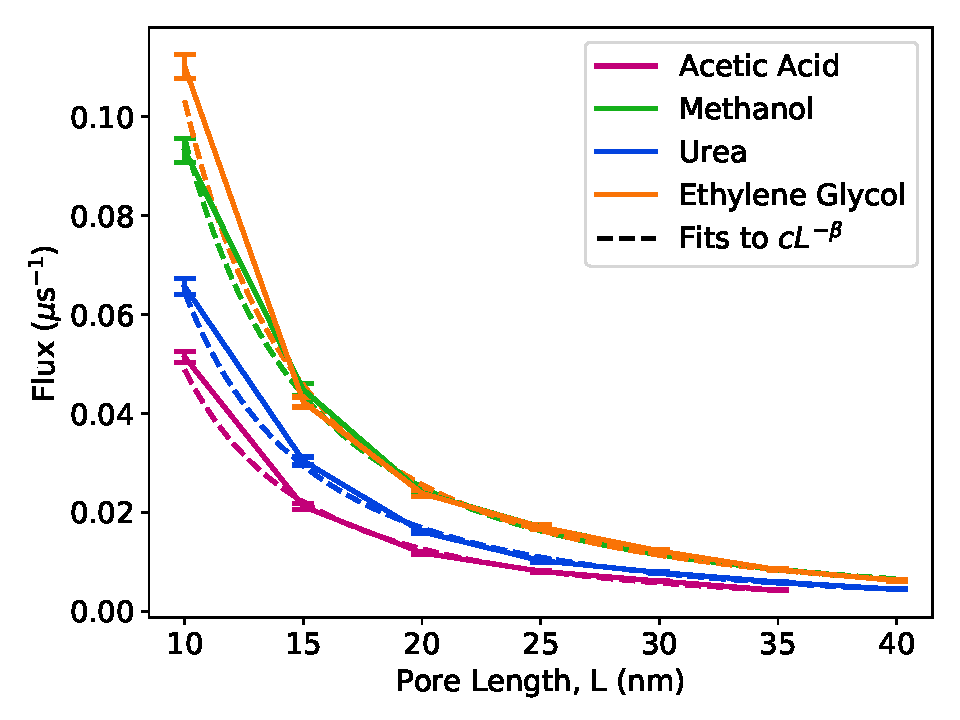
\includegraphics[width=\textwidth]{flux_curves_msddm.pdf}
  \caption{MSDDM}\label{fig:flux_curves_msddm}
  \end{subfigure}  
  %MRS6: make clear the dots are experiment. 
  \caption{(a) The distributions of first passage times generated from the sFBMcut model
  fit well to Equation~\ref{eqn:passage_times}. We show similar fits for the remaining
  solutes as well as the MSDDM in Figures~\ref{S-fig:ad_fpt_fits} and~\ref{S-fig:msddm_fpt_fits}
  of the Supporting Information. (b) The single particle flux measured 
  by the sFBMcut AD model and (c) the MSDDM decays with increasing pore length. 
  The rankings of solute fluxes are consistent with the MSDs predicted by each model.
  The ranking of the MSDDM is most consistent with MD MSDs. The MSDDM predicts higher
  fluxes than the sFBMcut model. We fit the single particle solute flux versus pore
  length, $L$, to a power law function of the form $cL^{-\beta}$ (dashed lines in (b)
  and (c)). 
%  Solutes with higher fluxes have higher values of $c$. Solutes with 
%  smaller Hurst parameters, $H$, have larger values of $\beta$. (c) If we remove 
%  correlation between hops (set $H$=0.5), the flux increases significantly and 
%  $\beta \sim 2$ for all solutes independent of dwell distribution
%  parameters.
  }\label{fig:flux_curves}
  \end{figure}
  
  
  % BJC: could use better color scheme. Maybe outline hurst parameters
%  \begin{subfigure}{0.475\textwidth}
%  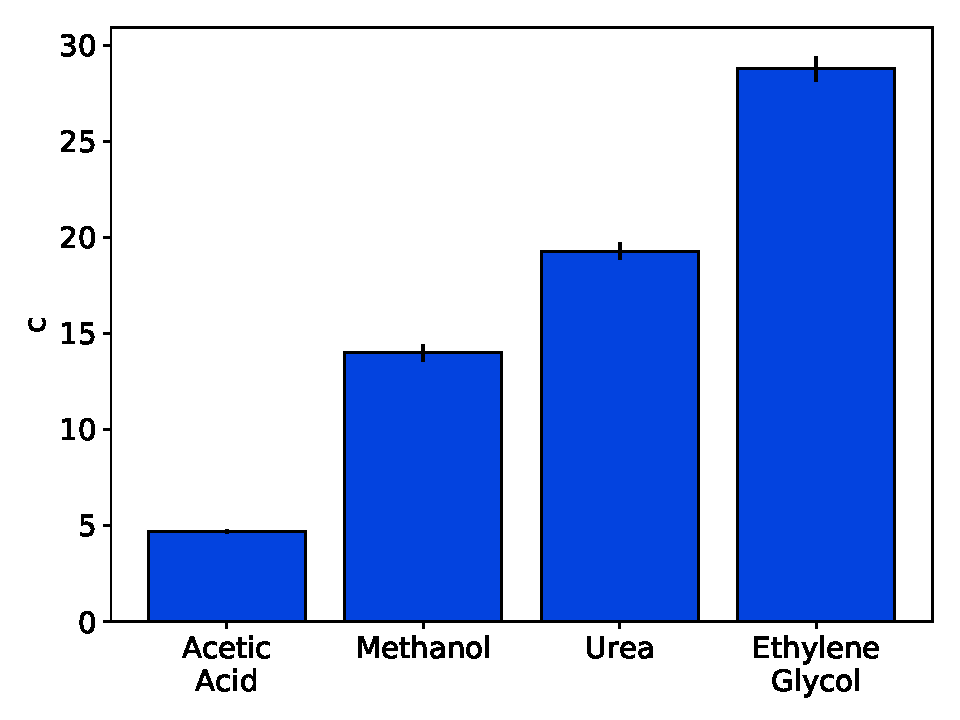
\includegraphics[width=\textwidth]{c_parameters.pdf}
%  \caption{}\label{fig:c_parameters}
%  \end{subfigure}
%  \begin{subfigure}{0.475\textwidth}
%  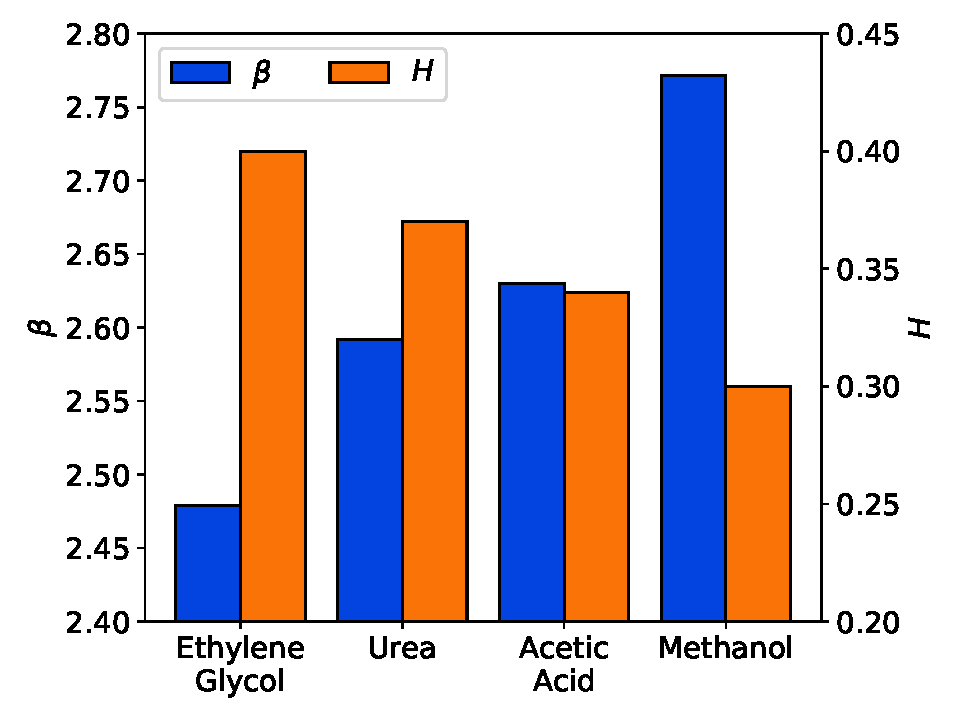
\includegraphics[width=\textwidth]{beta_parameters.pdf}
%  \caption{}\label{fig:beta_parameters}
%  \end{subfigure}
%  \begin{subfigure}{0.475\textwidth}
%  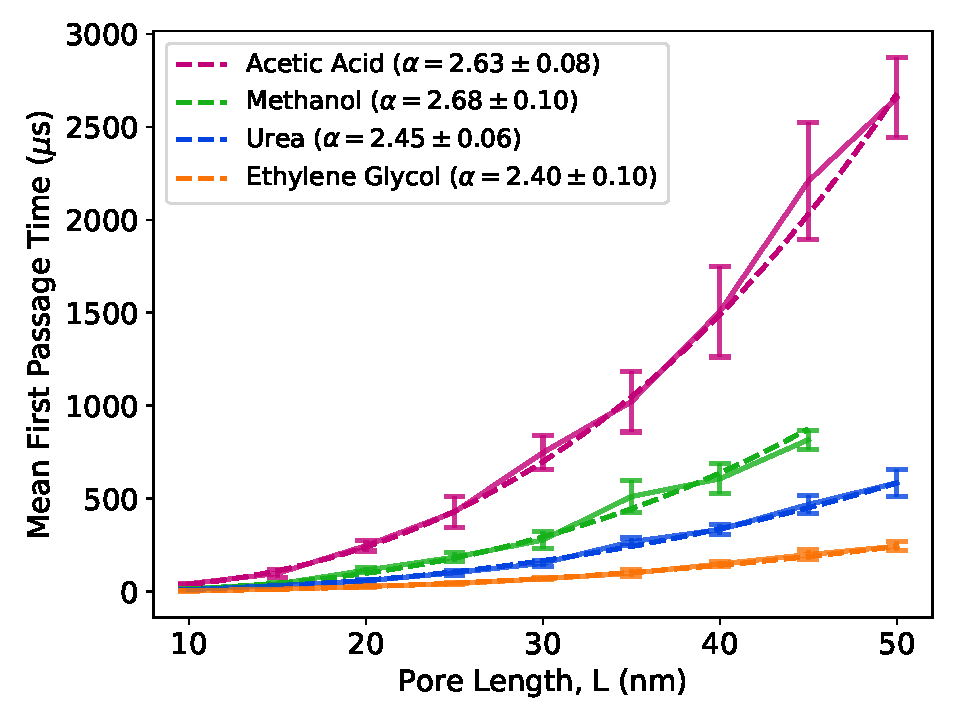
\includegraphics[width=\textwidth]{mfpt_curves.pdf}
%  \caption{}\label{fig:mfpt_curves}
%  \end{subfigure}
  %BJC: going out to 3 decimal places seems silly
  %BJC: might get closer to beta=2 if I use different curve fitting technique than fitting line to log-log
%  \begin{subfigure}{0.325\textwidth}
%  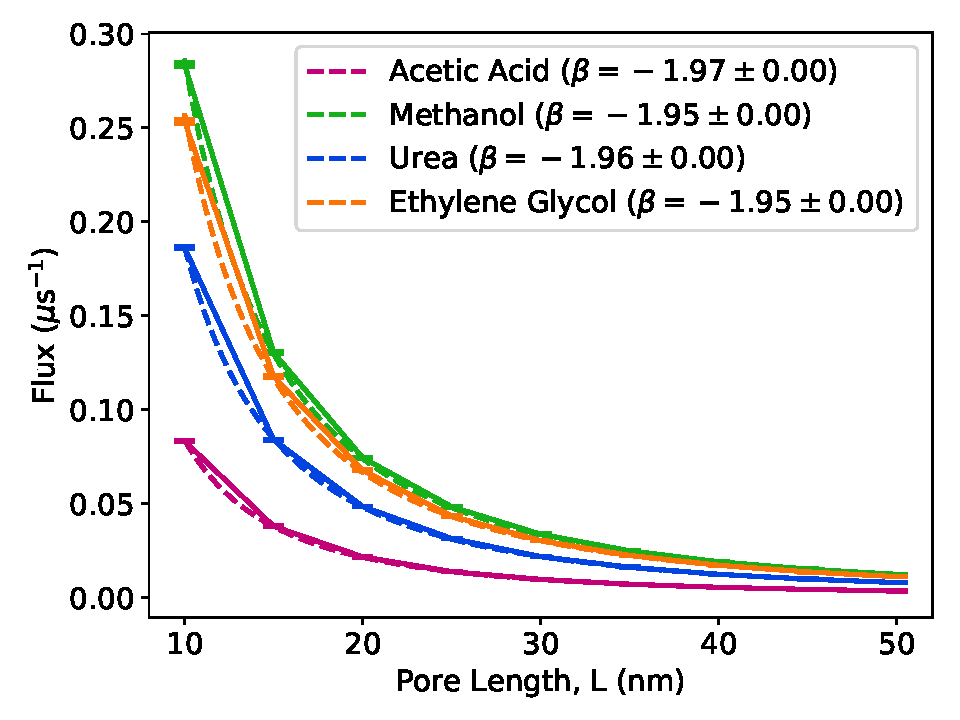
\includegraphics[width=\textwidth]{flux_curves_brownian.pdf}
%  \caption{Fixed $H=0.5$}\label{fig:flux_curves_brownian}
%  \end{subfigure}
%  \begin{subfigure}{0.475\textwidth}
%  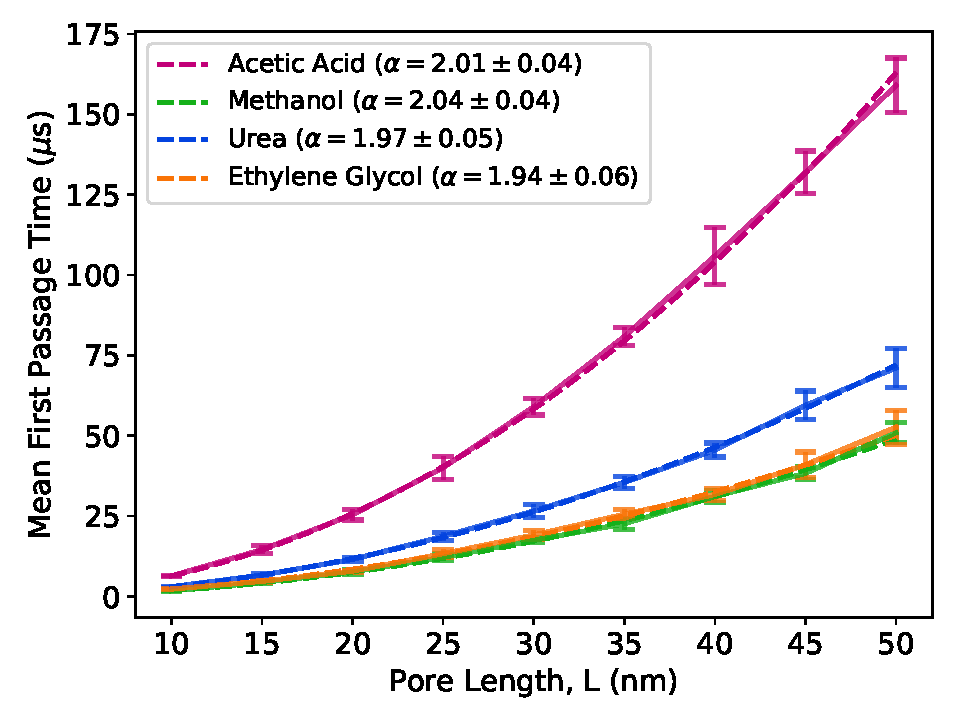
\includegraphics[width=\textwidth]{mfpt_curves_brownian.pdf}
%  \caption{}\label{fig:mfpt_curves_brownian}
%  \end{subfigure}
  %MRS5: the b) pane is a little messy.  If c) is moved to the supporting, maybe can make b into two figures, and 
  % have each just show 1 point? 

  We determined that it is only necessary to simulate 1000 realizations of each model
  in order to parameterize Equation~\ref{eqn:flux_decay}. We used 10000 trajectory
  realizations in order to generate each point in Figure~\ref{fig:flux_curves_ad}, 
  however, in Figure~\ref{S-fig:flux_curve_sensitivity} of the Supporting information,
  we show that one can still show statistically significant differences in solute 
  flux, with minimal change to the mean flux values, using as few as 100 trajectory
  realizations. 
  %To be sure, 
  For better precision, we recommend simulating at least 1000 realizations. 
  Since the computational cost of the MSDDM is greater than the AD model, we generated
  each point of the flux curves in Figure~\ref{fig:flux_curves_msddm} using only 1000
  realizations at each pore length. 
  
  %The scaling of solute flux with pore length is a complicated function of hop and 
  %dwell parameters, however, anti-correlation between solute hops appears to
  %be the most significant influencing factor. 
  The scaling of solute flux with pore length is primarily influenced by anti-correlation
  between solute hops. In Figure~\ref{fig:beta_hurst}, we show that $\beta$, as derived 
  from the sFBMcut model, is inversely related to the Hurst parameter. This makes intuitive
  sense since higher degrees of anti-correlation should slow the rate at which solutes
  cross the membrane pore. $\beta$, as derived from the MSDDM, appears approximately 
  constant but this is consistent with nearly invariant transitional Hurst parameters
  (see Figure~\ref{fig:H_v_state}). However, Figure~\ref{fig:beta_hurst} does raise
  the question as to why $\beta$ is so much lower than the sFBMcut model.
  
  To understand the behavior of the MSDDM, we studied the $\beta$ parameter derived 
  from variations on each model, visualized in Figure~\ref{fig:beta_parameters}. First, 
  we removed anti-correlation between hops in the sFBMcut trajectory (set $H$=0.5). 
  The $\beta$ parameter drops to values similar to the MSDDM. When we remove anti-correlation
  \textit{and} dwell times between hops (set dwell times equal to 1), effectively simulating 
  Brownian motion, we observe similar $\beta$ parameters. These two variations imply that,
  in the AD models, the $\beta$ parameter is only a function of $H$ and not dependent on
  dwell times ($\alpha_d$, $\lambda$) or hop lengths ($\sigma$). The MSDDM is fundamentally similar to 
  the AD model in that one makes correlated draws from a hop distribution. Therefore,
  we should expect the $\beta$ value of the MSDDM to be larger than that of Brownian 
  motion.
  %Although the dwell times are
  %insignificant compared to the AD model (compare Figures~\ref{fig:ad_eyetest} and
  %\ref{fig:msddm_eyetest} for example), we have just shown 
  
  The value of $\beta$ for the MSDDM is under-estimated due to assumptions of the model
  itself as well as inaccuracies in the correlation structure of very long FLM trajectories.
  Turning first to the model itself, we have designed it to ensure that the magnitude of the
  hops in the series of transitions between states are anti-correlated from start to finish. 
  This assumes that the transition correlation structure is unaffected by the
  sub-trajectories between each state transition. Each time a state transition occurs, one
  must initialize a new time series sub-trajectory with its own correlation structure. 
  %Even with a low Hurst parameter, as exhibited by most trapped states, the time spent 
  %in each state is relatively short making the accuracy of the correlation structure 
  %questionable. Additionally, $\sigma$ of transitional hops is similar in magnitude to
  %$\sigma$ in trapped states. 
  Since we add the transitional hop lengths to each end of
  trapped state sub-trajectories, the transitional hop lengths are shifted with respect 
  to one another, decreasing correlation between them. We tested this reasoning by modifying the 
  MSDDM to completely immobilize particles except when they transition between states. 
  Suprisingly, $\beta$ is still close to the Brownian value. Further experimentation 
  reveals that this is actually a consequence of the FLM simulation procedure. Simulating
  FLM requires Riemann-sum approximations of the stochastic integrals defining the process.
  To generate the curves in Figure~\ref{fig:flux_curves_msddm}, we needed to correlate 
  25--1000 times more hops than for the MSD predictions in Figure~\ref{fig:msddm_performance}. 
  In short, it is computationally infeasible to use enough terms to accurately incorporate
  long timescale correlations into our long MSDDM realizations. Thus at long timescales, 
  we lose correlation between transitional jumps. We confirmed this hypothesis by using 
  fractional Brownian motion, for which we have an exact simulation method, in place of 
  FLM in the MSDDM algorithm. When we use FBM, $\beta$ increases well above the Brownian 
  value. $\beta$ increases even further if we immobilize the trapped states. Thus the low
  value of $\beta$ of the MSDDM is a consequence of model assumptions and inexact simulation
  of FLM.  
  
  \begin{figure}
  \centering
  \begin{subfigure}{0.43\textwidth}
  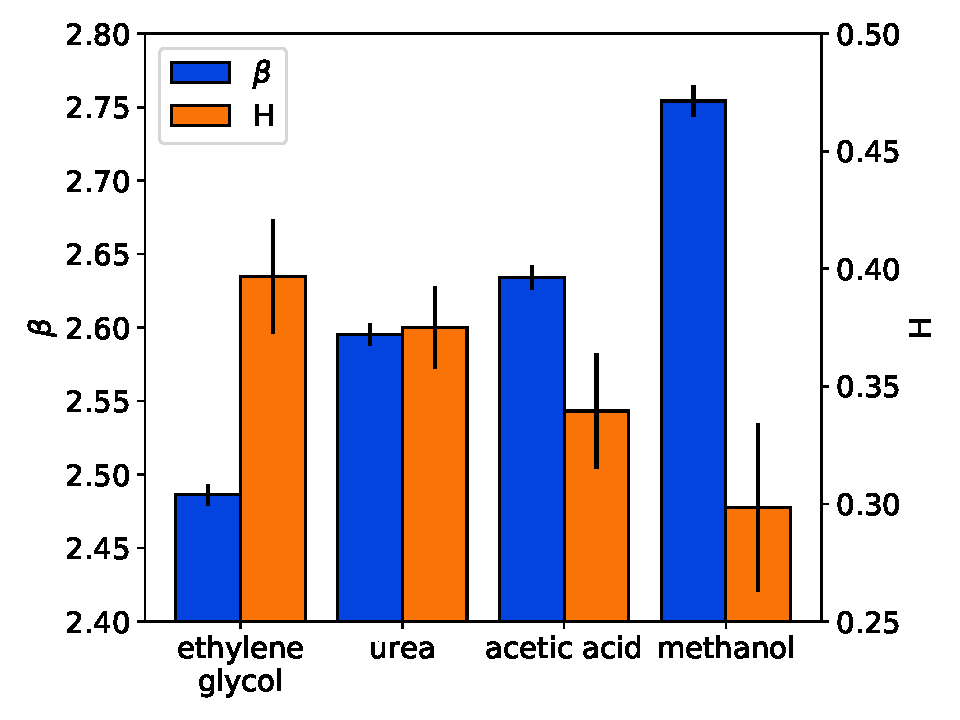
\includegraphics[width=\textwidth]{beta_hurst.pdf}
  \caption{}\label{fig:beta_hurst}
  \end{subfigure}
  \begin{subfigure}{0.52\textwidth}
  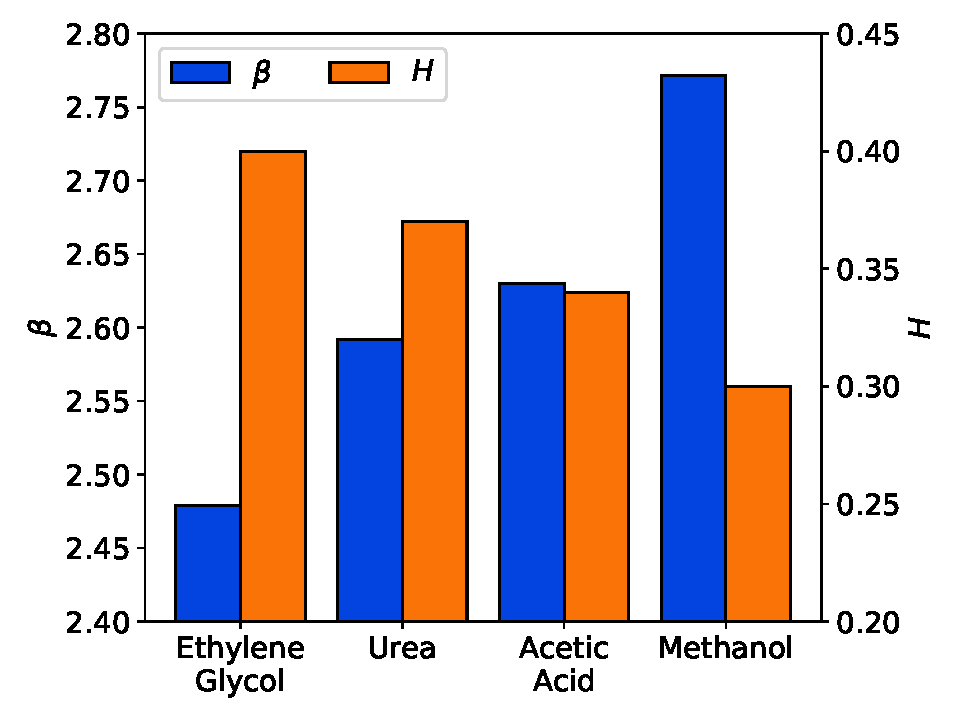
\includegraphics[width=\textwidth]{beta_parameters.pdf}
  \caption{}\label{fig:beta_parameters}
  \end{subfigure}
  %BJC5: need to update MSDDM (immobile states). Waiting on those simulations
  %MRS6: should try to lead with what the overall results/conclusions are.  What does it mean that parameters are larger or smaller?  What should the reader take from the discussion?  Should it be in supportinig?
  \caption{(a) The $\beta$ values of the sFBMcut model appear to be inversely proportional
  to the Hurst parameters. The $\beta$ values of the MSDDM are much lower with much less
  variation than the sFBMcut model. (b) The $\beta$ parameters of the MSDDM are low because
  sub-trajectories between state transitions decorrelate transitional hops and because
  our FLM simulation procedure does not accurately correlate hops after long time lags. 
  The high $\beta$ parameters of the sFBMcut model are a consequence of anti-correlation
  between hops. Removing hop correlations causes $\beta$ to drop down close to MSDDM
  values (sFBMcut ($H$=0.5)). Removing dwell times in addition to hop correlation
  yields a similar value of $\beta$ (Brownian). Immobilizing particles while in a trapped state
  also yields a similar value of $\beta$ (MSDDM (immobile states)). Replacing FLM with
  FBM in the MSDDM raises $\beta$ well above the Brownian value (MSDDM (FBM)). Replacing FLM with FBM and
  immobilizing particles in trapped states further raises the value of $\beta$.}\label{fig:beta}
  \end{figure}
  
  %MRS6: can this be made a physical thesis instead of a mathematical one?
  The values of $c$ are directly related to the magnitude of solute flux and, where
  applicable, are functions of $\sigma$, $\alpha_d$, $\lambda$ and $\alpha_h$. 
  In Figure~\ref{fig:c_parameters}, we plot the $c$ values measured
  for each solute with each model from lowest to highest. In general, $c$ values generated
  by the MSDDM model are smaller than the those generated by the sFBMcut AD model 
  because the AD model has to compensate for high $\beta$ values. Comparison 
  of Figure~\ref{fig:c_parameters} with Figures~\ref{fig:flux_curves_ad} 
  and~\ref{fig:flux_curves_msddm} reveals that the ranking of the $c$ parameters is
  consistent with the ranking of solute flux. Therefore, it is reasonable to hypothesize
  that any parameter which acts to modify the rate at which solutes move through the
  membrane pores will affect $c$ for various physical reasons. In 
  Figure~\ref{fig:c_influence} we demonstrate that decreased dwell times
  (increased $\alpha_d$), increased hop lengths (increased $\sigma$), cutting off the
  dwell time distribution at shorter times (increased $\lambda$) and increased tail 
  weights of the hop length distribution (decreased $\alpha_h$) independently lead to
  an increase in $c$. Figure~\ref{fig:c_influence} also suggests that $c$ is not dependent on hop
  anti-correlation ($H$).

%  We showed earlier that $\beta$ is not a
%  function of $\sigma$ or $\alpha_d$, therefore dwell times and hop lengths must
%  influence $c$. In fact, any parameter which acts to modify the rate at which 
%  solutes move through the membrane pores will affect $c$. Therefore it is 
%  sensible to hypothesize that a higher degree of anti-correlation (lower $H$)
%  should decrease $c$ and a higher value of $\alpha_h$ should also increase $c$.
%  In Figure~\ref{fig:c_influence}, we verify these hypotheses by holding 
  
  \begin{figure}
  \centering
  \begin{subfigure}{0.42\textwidth}
  % use c_parameters2.py
  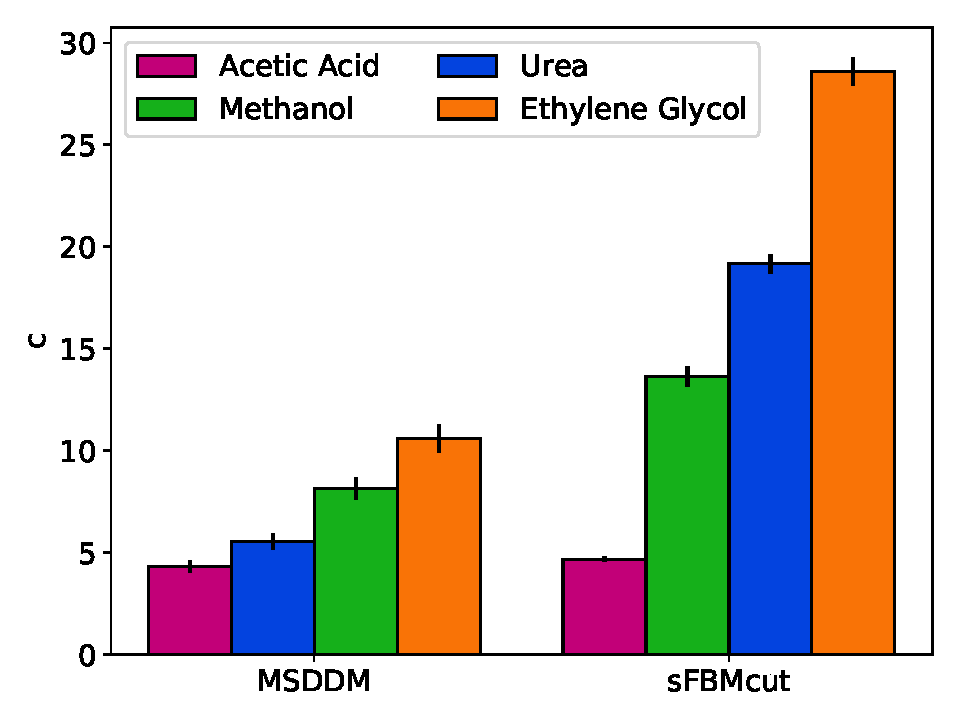
\includegraphics[width=\textwidth]{c_parameter_comparison.pdf}
  \caption{}\label{fig:c_parameters}
  \end{subfigure}
  \begin{subfigure}{0.53\textwidth}
  \vspace{0.5em}
  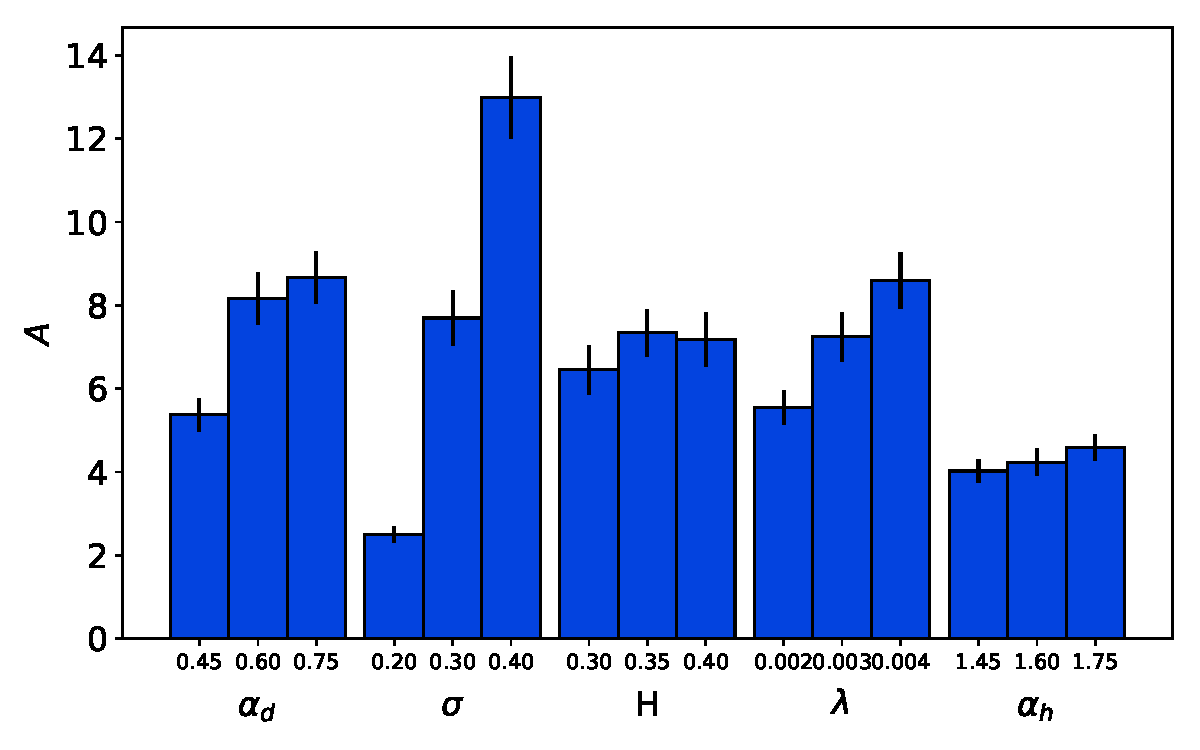
\includegraphics[width=\textwidth]{c_influence.pdf}
  \caption{}\label{fig:c_influence}
  \end{subfigure}
  %BJC5: waiting on simulations for alpha_h
  \caption{(a) The $c$ parameter increases with solute flux (compare ranking with
  Figures~\ref{fig:flux_curves_ad} and~\ref{fig:flux_curves_msddm}). The $c$ parameters
  of the MSDDM are smaller than the sFBMcut AD model because the AD model must
  compensate for its strong length dependence (higher $\beta$). (b) Changes to parameters
  which increase the rate of solute displacement result in larger values of $c$. 
  To test the dependence of $c$ on $\alpha_d$, $\sigma$, $H$ and $\lambda$, we chose a 
  single set of parameters, representative of solutes parameterized by the sFBMcut AD model,
  and generated realizations of the model by varying each parameter independently about the
  same base parameter set. Therefore, the middle bars for these four 4 parameters are 
  generated from the same set of parameters. Decreased dwell times (increased $\alpha_d$),
  increased hop lengths (increased $\sigma$), and a lower cut-off to the dwell time
  distribution (increased $\lambda$) lead to increases in $c$. $c$ responds linearly
  to increases in $\sigma$ and $\lambda$ and non-linearly to $\alpha_d$. The data 
  suggests that the $c$ parameters do not depend on hop anti-correlation ($H$). To test 
  $\alpha_h$, we used the set of parameters defining the MSDDM of Urea (since sFBMcut does
  not use a L\'evy distribution) and varied the $\alpha_h$ parameter of the transitional
  hops. As $\alpha_h$ increases, $c$ decreases since the probability of large hops decreases.
  We expect similar dependence of $c$ on $\sigma$ and $H$ of the MSDDM.}\label{fig:c}
  \end{figure}
  
%  \begin{figure}
%  \centering
%  % bar charts
%%  \begin{subfigure}{0.45\textwidth}
%%  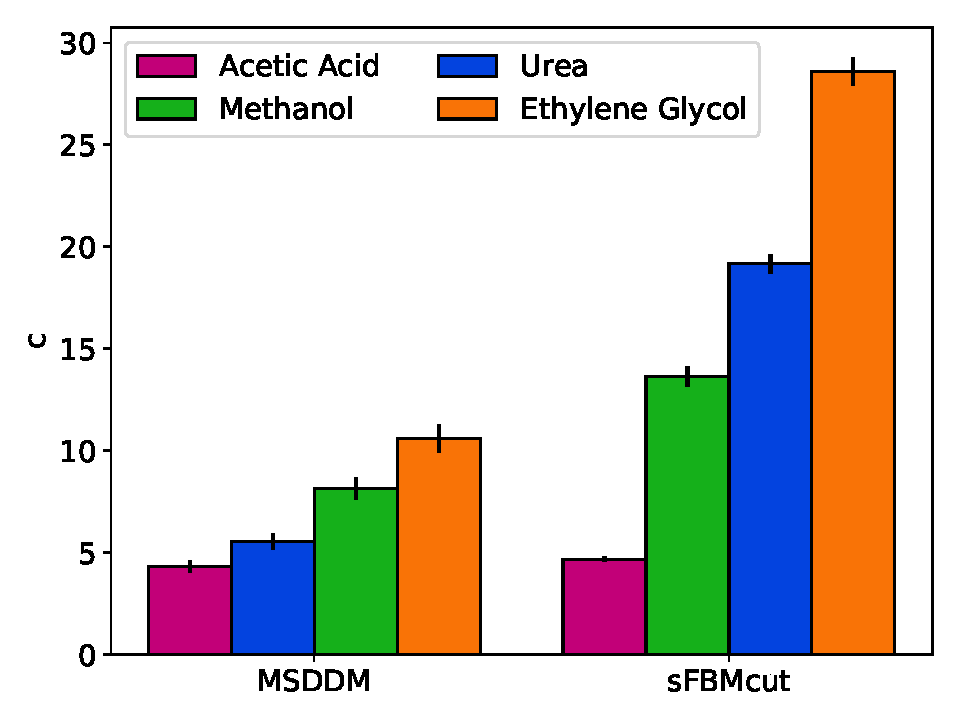
\includegraphics[width=\textwidth]{c_parameter_comparison.pdf}
%%  \end{subfigure}
%%  \begin{subfigure}{0.45\textwidth}
%%  \includegraphics[width=\textwidth]{beta_parameter_comparison.pdf}
%%  \end{subfigure}
%  \includegraphics[width=0.5\textwidth]{beta_c_parameter_comparison.pdf}
%  \caption{}\label{fig:flux_parameters}
%  \end{figure}

  %MRS5: probably the figure showing beta \sim 2 can be in supporting
  %information, and you just state the result here.
  %MRS: can you put a physical thesis here, not just a mathematical one?  Why is this change in parameters important to flux? 
%  The prefactor, $c$, in Equation~\ref{eqn:flux_decay} grows with increasing
%  solute MSD while the value of the growth exponent, $\beta$, is inversely 
%  related to the Hurst parameter, $H$ (see Figure~\ref{fig:flux_parameters}).
%  In Figure~\ref{fig:flux_curves_brownian}, we removed the correlation 
%  structure (set $H$=0.5) from AD trajectory realizations so that all hops 
%  were uncorrelated. Regardless of the parameters of the dwell time distribution,
%  the growth exponent is always about 2, the same value that we observe for 
%  Brownian motion (see Figure~\ref{S-fig:mfpt_curve_brownian} of the 
%  Supporting Information). 

% BJC: following is wrong
%  Dwell times between hops have a significant effect on the length dependence
%  of solute flux. The values of $\beta$ fit to realizations of the sFBMcut AD
%  model are significantly higher than the MSDDM. As evident by comparison of 
%  Figures~\ref{fig:msddm_eyetest} and~\ref{fig:ad_eyetest}, realizations of the
%  AD model exhibit much longer and more frequent periods of immobility. If we
%  generate realizations of the sFBMcut model without trapping (dwell times are
%  all 1 time step), the value of $\beta$ drops to 2 in all cases. In fact, we
%  observe the same value of $\beta$ for Brownian motion (see Figure blah of the 
%  Supporting Information) which implies that the Hurst parameter has no effect
%  on the length dependence of flux.
%  
%  Comparison of Figures~\ref{fig:flux_curves_regular} and~\ref{fig:flux_curves_brownian}
%  highlights that anti-correlation between hops plays a major role in solute flux.
%  With a pore length of 50 nm, the flux of the fasted moving solute, ethylene glycol is 
%  c.a. 5 times lower with versus without anti-correlated hops. The flux of the slowest
%  moving solute, acetic acid, is about 16 times lower by the same comparison. This 
%  difference will only grow with increasing pore length. Note also that the ranking
%  of solute fluxes changes. Methanol jumps from the second lowest to the highest
%  flux when we remove hop correlation. The high degree of anti-correlation among
%  hops made by methanol outweighs its relatively wide hop length distribution.
  
%MRS: can you connect directly to $\beta$ and $c$ here?  Important to
%make connections between macroscopic parameters and the molecular
%reason for them whenever possible.  Can combine with other paragraphs that talk mainly about c and beta.


%   In Figure~\ref{fig:mfpt_curves_regular} we show that the MFPT grows super-linearly
%  with pore length. We fit a curve of the form  to the curves in order
%  to estimate the growth exponent, $\alpha$. The growth exponent is inversely proportional
%  to the solute MSDs which is consistent with longer passage times for solutes that
%  progress through the pores more slowly.
  
  The power law decay of the flux with pore length implies the following relationship
  for selectivity via substitution of Equation~\ref{eqn:flux_decay} into 
  Equation~\ref{eqn:selectivity}:
  \begin{equation}
  S_{ij}(L) = \bigg(\frac{c_i}{c_j}\bigg)L^{(\beta_i - \beta_j)}
  \label{eqn:selectivity_ratio}
  \end{equation}
  
  %MRS5: figure seem to show that the selectivity plateaus more or less, so thin coatings enough. 
  In Figure~\ref{fig:selectivity}, we plot Equation~\ref{eqn:selectivity_ratio} for pore
  lengths ranging from those studied in Figure~\ref{fig:flux_curves} to macroscopic-length
  pores. Greater differences in $\beta$ values leads to selectivities that are stronger 
  functions of pore length. For $(c_i / c_j)=1$, LLC membranes will be more selective
  towards passage of solutes with lower $\beta$ values versus those with high $\beta$ values.
  When $\beta$ values are equal, as is the case for uncorrelated motion, selectivity only
  depends on the pre-factors, $c$. In most cases, the length dependence of selectivity 
  plateaus quickly which implies that a coating of LLC membrane with a thickness on the 
  order of those already made experimentally should be sufficiently optimal. 
  %MRS5? can you remind people of the physical source (in terms of dwell times, hop lengths) of the differences in beta and c? Want to try to stablish the connection between particle dynamic behavior and selectivity. 

  \begin{figure}
  \centering
  \begin{subfigure}{0.45\textwidth}
  \includegraphics[width=\textwidth]{selectivity.pdf}
  \caption{sFBMcut}
  \end{subfigure}
  \begin{subfigure}{0.45\textwidth}
  \includegraphics[width=\textwidth]{selectivity_msddm.pdf}
  \caption{MSDDM}
  \end{subfigure}
  \caption{The selectivity of 2 species changes monotonically with pore length. The
  strength of dependence on pore length depends on the difference between $\beta$ values.
  The selectivities predicted by the sFBMcut AD model (a) are much larger in magnitude than
  those predicted by the MSDDM (b) because predictions of the AD model result in a much
  larger variation in flux (compare Figures~\ref{fig:flux_curves_ad} and~\ref{fig:flux_curves_msddm}).}
  \label{fig:selectivity}
  \end{figure}
  
  The selectivities predicted by the sFBMcut model are both higher in magnitude and
  ordered differently than the those predicted by the MSDDM. The magnitudes of the
  sFBMcut predictions are higher because the predicted solute fluxes vary more widely
  than those predicted by the MSDDM (compare Figures~\ref{fig:flux_curves_ad} 
  and~\ref{fig:flux_curves_msddm}). The ordering is different mostly because the 
  ordering of the flux predictions is different. 
  
  We cannot say with absolute certainty which selectivity curves are more 
  trustworthy. The sFBMcut model uses exact simulation techniques and yields 
  qualitatively accurate solute trajectories, but it may overestimate long 
  timescale correlation present in the real system. For this reason, we might
  expect the $\beta$ values of the true flux curves to be closer to the 
  Brownian value as exhibited by the MSDDM. But the MSDDM yields qualitatively
  inaccurate solute trajectories and we do not have a good understanding of
  how to precisely control the point at which solute hops become decorrelated.
  
  However, we may gain the most by using the two models in tandem. In both cases,  
  the data suggests that this particular LLC membrane might be most useful for 
  selectively separating ethylene glycol from acetic acid. Ethylene glycol
  exhibits the highest flux while acetic acid has the lowest. Ethylene glycol
  has the weakest dependence on pore length (lowest $\beta$) according to the
  sFBMcut model, while acetic acid has the second highest dependence. This 
  analysis certainly merits further experimental exploration.

  
%  Out of the solutes studied, the data suggests that this particular LLC membrane 
%  %MRS5: would is a bit strong given the number of limitations.
%  %would 
%  might
%  be most useful for selectively separating ethylene glycol from methanol and 
%  acetic acid. 
%  %It also shows reasonable selectivity of Urea over acetic acid.  
%  Ethylene glycol has the highest $c$ value and the lowest $\beta$ value. The high
%  value of $c$ itself greatly enhances its selective passage. Even more importantly,
%  the relatively large difference between its $\beta$ value and those of methanol 
%  and acetic acid give rise to a strong pore length dependence. The selectivity is
%  enhanced as the pore length increases at the cost of lower solute flux, a 
%  phenomenon ubiquitous in polymer separations membranes.~\cite{geise_water_2011}

%  BJC4: Uncomment to see MFPT curves
%  \begin{figure}
%  \centering
%  \begin{subfigure}{0.325\textwidth}
%  \includegraphics[width=\textwidth]{mfpt_curves.pdf}
%  \caption{Correlated Hops}\label{fig:mfpt_curves_regular}
%  \end{subfigure}
%  \begin{subfigure}{0.325\textwidth}
%  \includegraphics[width=\textwidth]{mfpt_curves_brownian.pdf}
%  \caption{Uncorrelated Hops}\label{fig:mfpt_curves_brownian}
%  \end{subfigure}
%  \begin{subfigure}{0.325\textwidth}
%  \includegraphics[width=\textwidth]{frac_pore.pdf}  % This figure might fit in earlier
%  \caption{}\label{fig:frac_pore}
%  \end{subfigure}
%  \caption{(a) We fit the MFPT versus pore length to a function of the form $cL^{\alpha}$. 
%  The MFPT grows super-linearly with increasing pore length. Solutes with lower MSDs have
%  higher MFPTs. (b) If we remove correlation between hops, the MFPTs reduce significantly
%  and the growth exponent stays constant at 2 for all solutes independent of dwell
%  distribution parameters. Higher degrees of anti-correlation (lower $H$) lead to higher
%  growth exponents. (c) Solutes that spend a large fraction of their time in the tails tend
%  to have larger Hurst parameters.}\label{fig:mfpt_curves}
%  \end{figure}
  
%  In Figure~\ref{fig:frac_pore}, we show that solutes which spend more time in the tails
%  tend to have lower Hurst parameters. The densely packed, viscoelastic alkane chains 
%  bounce solutes between them, severely limiting their mobility. Designing LLC membranes
%  that can control or prevent the partition of solutes into the tails may offer the highest
%  returns on membrane performance.
  
  %BJC: can make design suggestions by trying to decrease anticorrelation by x
  
%  In this section, we use our most promising models to predict solute flux 
%  through a theoretical 50 nm channel. For our comparisons to MD, using a truncated
%  power law distribution is an obvious choice. However, given that extremely
%  long dwells are a rare event, it is possible that studying a much larger set of 
%  solutes will fill in the tail of the pure power law PDF. Regarding hop length 
%  distributions, the generality of L\'evy stable distributions is powerful, but the
%  lack of exact methods for simulation of fractional L\'evy motion reduces it's 
%  accuracy and computational tractability. Treating the dynamics as fractional 
%  Brownian motion is probably sufficient unless the L\'evy index, $\alpha_h$, is 
%  well below 2.
%  
%  Choosing which model to use for long timescale projections is not entirely obvious
%  without experimental data to compare with. 
  
%  We projected the long timescale behavior using this model. 

  \section{Conclusions}
  
  We have tested two different mathematical frameworks for describing solute
  motion by applying them to an H\textsubscript{II} phase LLC membrane. The values
  obtained for the parameters when fitting the models to the time series data 
  offer important mechanistic insight on the molecular details of transport.
  Subordinated fractional Brownian and L\'evy motion have a 
  %nice 
  strong theoretical 
  foundation in the anomalous diffusion literature. Our single mode model
  quantifies and allows comparison of the hopping and trapping behavior 
  among solutes. A two mode model that describes dynamics based on whether
  a solute is in or out of the pore region allows us to break down individual
  solute motion into the two distinct regimes and we showed that solute motion is
  clearly restricted while in the tail region. Our Markov state-dependent dynamical
  model uses explicitly defined trapping mechanisms and gives a nice description 
  of transitions between these observed states, the equilibrium distribution of 
  solutes among states as well as the type of stochastic behavior shown in each 
  state. 
  
  %MRS6: right answer, wrong reason for MSD match issue?
  All of the models we tested have moderate success reproducing the MSDs of
  solute trajectories generated by MD simulations. In almost all cases, large 
  portions of the MSDs predicted by our models fall close to or within the 1$\sigma$
  confidence intervals of MD. Aside from inaccuracies in parameter estimates,
  the most significant shortcoming of all of our models is their ability to 
  accurately portray the curvature of the MSD curves. The MD MSD curves tend to 
  become linear on long timescales, but the MSD curves generated by our models
  have persistent curvature that causes them to under-predict the MSD on very
  long timescales. This is a consequence of the correlation structure associated
  with fractional motion. In the future, we could address this by 
  implementing a truncation to the positional autocorrelation function.
  
  We demonstrated how one could used our models in order to to determine
  macroscopic flux and selectivity. We showed that, when using the AD model, 
  solute flux decreases with pore length at a rate faster than pure 
  Brownian motion due to anti-correlation between hops. However, using the
  MSDDM, we observed a decay in flux similar to Brownian motion. This is
  primarily due to the inexact method that we use to correlate hops of the 
  fractional L\'evy motion process. When we replace FLM with FBM in the 
  MSDDM algorithm, we observe a flux decay more consistent with that predicted
  by the AD model. Finally, we used the ratio of solute fluxes in order to
  calculate selectivity. Due differences in hop anti-correlation, we observe
  a length dependent selectivity. However, this length dependence mostly
  plateaus at length scales that can be synthesized experimentally. The data
  suggests that this particular membrane may be useful for separating
  ethylene glycol and acetic acid.

  % BJC5: I'm not sure if this paragraph belongs here. Or if it should go at end
  % of previous section. Or just eliminate. What do you think?  
  Of course, our approach to modeling LLC membrane selectivity neglects a number
  of factors that influence real-world aqueous membrane separations. The most 
  glaring is that we neglected convective flux which should work to increase 
  overall solute flux and lower selectivity (see Equation ~\ref{eqn:solute_flux}).
  Defects in the pore structure will have a strong influence on solute flux which
  may exacerbate the length dependence of flux. Even in a perfectly structured 
  membrane, the barrier to pore entry from the bulk solution will have its own 
  influence on experimentally observed selectivities. This energetic barrier can 
  be made even worse by foulants deposited on the membrane's surface. Therefore,
  our predictions should be primarily used to identify the most promising types
  of selective separations for an H\textsubscript{II} LLC membrane made from a 
  specific monomer.

  Our mathematical models help us think about how to design LLC monomers for 
  solute-specific separations by forcing us to think in terms of controlling 
  solute trapping. The anomalous diffusion model is quite flexible because it
  does not require knowledge of specific trapping mechanisms. Screening a set
  of solutes and applying the anomalous diffusion model can help uncover
  trapping mechanisms by forcing the scientist to identify features common 
  to solutes with long or short hop lengths and dwell times. The MSDDM is a 
  powerful way to characterize explicit trapping mechanisms. It clearly
  partitions a trajectory into discrete mechanisms and quantifies their
  relative dominance in the real system. For example, it is clear that 
  sodium ion association is primarily responsible for trapping urea while 
  hydrogen bonding dominates ethylene glycol. If one re-designs an LLC monomer
  to eliminate one source of trapping, then high selectivities are possible.
  Overall, in tandem or separately, our models facilitate new ways of approaching
  complex separation problems.
  
%  Properly parameterizing
%  and simulating the correlation structure of the time series is very important. 
%  Based on physical intuition, we assumed the correlation to be a consequence of 
%  a fractional process however, autoregressive techniques may offer a more flexible
%  approach.
% Both models describe the trapping mechanism in
%  different ways. The anomalous diffusion model does not consider mechanisms but
%  insight into the length of entrapment
%  
%  The anomalous diffusion gives clues to the type 
%  of functionality that leads to long dwell times. It is readily apparent that solute 
%  
%  One must consider how to control them and 
%  a solute's preference towards the pore or tail region. 
%  They can dissect solute movement down to their 
%  individual positional fluctuations and give information about the influence 
%  of the surrounding chemical environment. 
%
%  
%  Combined with qualitative studies of solute transport to aid in model construction,
%  our stochastic modeling framework can be used to quantitatively dissect the dynamic
%  behavior of solutes in LLC membranes. Our work demonstrates that when designing a membrane for a 
%  specific separation, one must consider the types of trapping mechanisms that 
%  may play a role in transport, how solutes partition in the membrane,
  
  
  \section*{Supporting Information}

  Detailed explanations and expansions upon the results and procedures mentioned in
  the main text are described in the Supporting Information. This information is
  available free of charge via the Internet at http://pubs.acs.org.

  \section*{Acknowledgments}
  %MRS: add people who contributed non-author level ideas. 
  %MRS3: add specific info for PRF and GAANN
  %BJC3: I wrote GAANN as I did on the last paper which is what Rob Davis told me to do
  This work was supported in part by the ACS Petroleum Research Fund grant \#59814-ND7
  and the Graduate Assistance in Areas of National Need (GAANN)
  fellowship which is funded by the U.S. Department of Education.
  Molecular simulations were performed using the Extreme Science and
  Engineering Discovery Environment (XSEDE), which is supported by National
  Science Foundation grant number ACI-1548562. Specifically, it used the Bridges
  system, which is supported by NSF award number ACI-1445606, at the Pittsburgh
  Supercomputing Center (PSC). This work also utilized the RMACC Summit supercomputer,
  which is supported by the National Science Foundation (awards ACI-1532235 and
  ACI-1532236), the University of Colorado Boulder, and Colorado State
  University. The Summit supercomputer is a joint effort of the University of
  Colorado Boulder and Colorado State University.
  
  We would also like to thank Richard Noble for helping us make the connection 
  between the empirical mean first passage time distribution and the analytical
  equation to which we fit the distributions (Equation~\ref{eqn:passage_times}).
  

  \clearpage

  %MRS6: look over and make bibliography consistent (i.e. no months, consistent journal abbreviations)
  \bibliographystyle{ieeetr}
  \bibliography{stochastic_transport}

  \newpage

  \section*{TOC Graphic}
    
  %BJC5: still a work in progress
  %MRS6: seems pretty reasonable as a concept. If you can make the three figure labels the same color (doesn't have to be black or white) and same font, might be nice.  Maybe make arrows more like circle arcs, and change the color from black so it stands out more?  The time series model figure is a bit busy. Can it be reduced from 4 subfigures?  May not be necessary, but one thing to think about.
  \begin{figure}[!htb]
  \centering
  \includegraphics[width=3.25in]{toc.pdf}
  \end{figure}

\end{document}

% LocalWords:  solute MSDs solutes solute's LLC BJC nanoporous maginn Lyotropic
% LocalWords:  micropollutants LLCs amphiphilic mesophases feng Bicontinuous EG
% LocalWords:  permeability hatakeyama zhou resel selectivities Edisonian CTRW
% LocalWords:  subdiffusive timescale timescales subdiffusion FBM RWF metzler
% LocalWords:  jeon neusius pdf Sokolov ony MSD MSMs chodera MSM AcOH URE MeOH
% LocalWords:  Hbonding hbonds hbond GROMACS berendsen gromacs der spoel hess
% LocalWords:  wt Na GA carboxylate Parrinello Rahman barostat rescale msd dt
% LocalWords:  superdiffusive EB sFBM min Hurwitz factoid MLEs autocovariance
% LocalWords:  evy sFLM FLM sFLMcut Dirichlet saiid fbm Stoev Taqqu MLE TODO SI
% LocalWords:  vvvv wehmeyer MSMbuilder pyEMMA featurization Phys Chem bayesian
% LocalWords:  Markovianity MSDDMs MSDDM resampling TBD MSD's CTRWs GCL acf ACH
% LocalWords:  urea's alkane overlayed SFLMcut underpredicted Gaussians HMM PRF
% LocalWords:  params msddm timeseries overpredicted GAANN ACS XSEDE ACI PSC
% LocalWords:  RMACC TOC
